\documentclass[doc,floatsintext]{apa6}

\usepackage{babel}
\usepackage{csquotes}
\usepackage{apacite}
\usepackage[T1]{fontenc}
\usepackage{lmodern}
\usepackage[utf8]{inputenc}
\usepackage{amssymb}
\usepackage{amsfonts}
\usepackage{amsmath}
\usepackage{graphicx}
\usepackage{float}
\usepackage{caption}
\usepackage{subcaption}
\usepackage{enumitem}
\usepackage[section]{placeins}
\usepackage[textsize=tiny]{todonotes}
\setlength{\marginparwidth}{2cm}

% ---------- watermark -----------
\usepackage[firstpage]{draftwatermark}
\SetWatermarkAngle{0}
\SetWatermarkFontSize{0.25cm}
\SetWatermarkVerCenter{0.75cm}
\SetWatermarkLightness{0.5}
\SetWatermarkHorCenter{14cm}
\SetWatermarkText{\shortstack[l]{
Tauber, S., Navarro, D. J., Perfors A. and Steyvers, M. (2017). Bayesian models \\
of cognition revisited: Setting optimality aside and letting data drive psychological \\
theory. Psychological Review, 124, 410-441. https://doi.org/10.1037/rev0000052
}}
\SetWatermarkScale{1}
% -------------------------------

\newcommand{\mink}{{Min\textit{k}\ }}
\newcommand{\CITE}{{\bf[CITE]}}
\newcommand{\CITETHIS}[1]{{\bf[CITE: #1]}}
\newcommand{\bigh}{\mathcal{H}}
\newcommand{\be}{\begin{equation}}
\newcommand{\ee}{\end{equation}}
\newcommand{\given}{\ | \ }
\newcommand{\TODO}[1]{ {\bf [TODO: #1] } }
\newcommand{\stimulus}[1]{\textsc{#1}}

\providecommand{\vbars}[1]{\lvert#1\rvert}

\title{Bayesian models of cognition revisited: Setting optimality aside and letting data drive psychological theory}
\shorttitle{Bayesian models of cognition revisited}

\fourauthors{\normalsize Sean Tauber}{\normalsize Danielle J. Navarro}{\normalsize Amy Perfors}{\normalsize Mark Steyvers}
\fouraffiliations{School of Psychology\\University of New South Wales}{School of Psychology\\University of New South Wales}{School of Psychology\\University of Adelaide}{Department of Cognitive Sciences\\University of California, Irvine}

\leftheader{Bayesian models of cognition revisited}

\abstract{Recent debates in the psychological literature have raised questions about the assumptions that underpin Bayesian models of cognition and what inferences they license about human cognition. In this paper we revisit this topic, arguing that there are two qualitatively different ways in which a Bayesian model could be constructed. The most common approach uses a Bayesian model as a normative standard upon which to license a claim about {\it optimality}. In the alternative approach, a {\it descriptive} Bayesian model need not correspond to any claim that the underlying cognition is optimal or rational, and is used solely as a tool for instantiating a substantive psychological theory. We present three case studies in which these two perspectives lead to different computational models and license different conclusions about human cognition. We demonstrate how the descriptive Bayesian approach can be used to answer different sorts of questions than the optimal approach, especially when combined with principled tools for model evaluation and model selection. More generally we argue for the importance of making a clear distinction between the two perspectives. Considerable confusion results when descriptive models and optimal models are conflated, and if Bayesians are to avoid contributing to this confusion it is important to  avoid making normative claims when none are intended.}

\keywords{Bayesian cognitive models; Bayesian data analysis; rational analysis; optimal predictions; generalization; inductive reasoning}

\begin{document}
\maketitle


\section*{Introduction}

Over the last two decades, Bayesian models have emerged as a powerful tool for understanding human cognition. Taking inspiration from Marr's \citeyear{marr_vision_1982} notion of computational level models and Anderson's \citeyear{anderson_adaptive_1990} outline of a rational analysis, the key idea is to take a top-down view of model construction. Within this program, human cognition is viewed in terms of the solution to a computational problem posed by the environment in which humans operate. This approach to cognitive modeling has been successfully applied to a wide range of problems in concept learning \cite{tenenbaum_bayesian_1999}, reasoning \cite{oaksford_rational_1994}, causal inference \cite{griffiths_structure_2005}, perception \cite{knill_perception_1996,shen2016}, motor control \cite{kording_bayesian_2004}, social cognition \cite{baker_action_2009}, decision making \cite{vul_one_2014}, language acquisition \cite{perfors_learnability_2011}, and many more besides. In general, computational-level analyses can take many forms. The existing literature includes analyses that rely on information theory \cite<e.g.,>{navarro_hypothesis_2011}, reinforcement learning \cite<e.g.,>{NavarroSUB}, algorithmic complexity theory \cite<e.g.,>{chater_generalized_2003_FIXED}, and statistical decision theory \cite<e.g.,>{vul_one_2014}, among others. However, the majority of computational-level analyses are framed in {\it Bayesian} terms.

Bayesian analyses typically approach human learning and reasoning by assuming that the learner's task is to infer which hypothesis $h$ among many possibilities best characterizes the world. The collection of possible hypotheses $\bigh$ is referred to as the {\it hypothesis space}, and the learner's pre-existing beliefs are captured by a {\it prior distribution} $P(h)$. Upon encountering data $x$, the learner updates her beliefs to a {\it posterior distribution} $P(h|x)$ via Bayes' rule:
\be
P(h|x) = \frac{ P(x|h) P(h) }{\sum_{h^\prime \in \bigh} P(x|h^\prime) P(h^\prime)}
\label{eq:bayes}
\ee
This belief updating rule relies heavily on the {\it likelihood function} $P(x|h)$, which describes the probability that the learner would have observed data $x$ if hypothesis $h$ were true. The likelihood function is what allows the learner to make inductive leaps, transforming her prior beliefs $P(h)$ into posterior beliefs $P(h|x)$ that have been informed by data. One of the distinctive characteristics of the Bayesian framework for cognitive modeling is the fact that belief revision via Bayes' rule is often described as a uniquely coherent way to reason rationally from data \cite<e.g.,>{jaynes_probability_2003}, a virtue that is reflected in the growing psychological literature on Bayesian data analysis \cite<e.g.,>{lee_bayesian_2014,kruschke_doing_2010,rouder_default_2012}.

Highlighting the success of the framework, there are now a number of tutorial articles \cite{perfors_tutorial_2011} and overviews \cite{tenenbaum_theory-based_2006}, as well as a number of papers articulating concerns and disagreements with the Bayesian approach \cite{jones_bayesian_2011,bowers_bayesian_2012,marcus_how_2013, CasseySUB}, defences of the paradigm \cite{chater_imaginary_2011,griffiths_how_2012,goodman_relevant_2015}, and responses to those defences \cite{bowers_is_2012,marcus_still_2015,jones_pinning_2011}. The scope of this debate is broad, but two concerns in particular stand out in these discussions. First, critics of the Bayesian approach frequently take issue with substantive claims about the optimality of human cognition. Second, a common criticism is that Bayesian models are too unconstrained, and that virtually any pattern of behavior can be accommodated by a suitably-formulated Bayesian model. The two criticisms combine to produce the worry that Bayesian models of cognition make a central claim about optimality that is unfalsifiable: that it is always possible to ``prove'' that humans are rational by judicious choice of priors and likelihoods. If this were true, the result would be a modeling framework that is not only vacuous, but also does not make an interesting claim about human psychology.

This critique exposes a degree of tension in how Bayesian models are constructed and the scientific inferences they license about human cognition. Our claim is that there are two quite different ways of thinking about Bayesian cognitive models: A model might act as a normative standard against which human cognition is measured, or it might serve as as a descriptive tool used to instantiate theories about human cognition \cite<see, e.g.,>{mckenzie_rational_2003}. In this paper we argue that the differences between these two perspectives can lead researchers to construct models with very different characteristics. With this in mind, we suggest that it would be useful to make a clear distinction between {\it optimal} Bayesian cognitive models that specify normative standards and license claims about the rationality of human cognition, and {\it descriptive} Bayesian cognitive models that may serve other theoretical goals but do not necessarily have much to say about whether human cognition is rational.

One reason for introducing the distinction between optimal and descriptive models  is that it is not always obvious when a Bayesian model is intended to imply a normative claim and when it is not: The same terminology is used to describe Bayesian models no matter what implications those models might have for the optimality of human cognition. A second reason for doing so is that it motivates an examination of what role a Bayesian model can play when it is used as a purely descriptive tool, rather than serving as a vehicle for arguments over whether people are ``rational''. By deliberately setting aside any claims to optimality, a descriptive Bayesian approach shifts the research focus away from questions about rationality or optimality, and onto more traditional psychological questions. What biases and beliefs do people bring to a task? (questions about priors) How do people update their knowledge in light of new data? (questions about likelihoods) What representations do people have? (questions about hypothesis spaces) Within the descriptive framework it is possible to learn about these questions by performing inference on those aspects of the model directly, rather than indirectly and in a more {\it ad hoc} way by setting them and examining model fit. The descriptive approach offers a vision for Bayesian cognitive modeling that disentangles the formal apparatus of Bayesian models (with their use of priors, likelihoods, and hypothesis spaces, all of which we want to keep) with the claims about rationality which---while an important foundation of the optimal Bayesian approach---are not required in the descriptive approach.

Our goal in this paper is not to argue for the superiority of either kind of Bayesian model---normative standards and descriptive models are both useful tools for cognitive scientists---but to try to highlight the importance of maintaining a clear distinction. This distinction is theoretical more so than methodological: Although the descriptive approach is much more flexible---and therefore allows for a wider range of methodological approaches to parameter estimation and model selection---this flexibility is \textit{the result} of letting go of optimal interpretations and the constraints that come with them.

With this in mind, we present three illustrative case studies, each chosen to highlight different ways in which the descriptive approach can enable modelers to ask {\it different} questions than a Bayesian model that focuses on questions of optimality.  Our examples show that a descriptive approach allows the researcher to use empirical data to robustly learn the mental representations that underpin human performance. We demonstrate how it can be used to investigate the biases and mental representations that shape human judgments as well as the learning rules that people use to change those beliefs. We examine how individual differences in cognition can be explored within the data-driven, descriptive Bayesian approach. Finally, our examples show that the insights obtained with a descriptive approach can be compared and contrasted with the findings of an optimal model---sometimes lending support and sometimes standing in opposition---or that they can stand alone without consideration to questions of optimality.

\subsection*{What makes a Bayesian model optimal?}

A natural place to begin the discussion is with a consideration of why Bayesian models are often claimed to represent rational or optimal inference. Critics of the Bayesian framework have sometimes assumed that Bayesian cognitive models exist to support normative claims about the optimality or rationality of human cognition  \cite{bowers_bayesian_2012,marcus_how_2013}, citing as their justification the fact that Bayesians very frequently do talk in precisely these terms \cite<see>[for examples]{bowers_is_2012}. Yet, as defenders of the Bayesian approach have noted in their commentaries, considerable care is required when making any claim about optimal performance \cite<e.g.,>{griffiths_how_2012}. Arguments for the optimality of Bayesian reasoning {\it in general} do not imply that every Bayesian model will make good predictions solely by virtue of being Bayesian: The optimality of any {\it particular} Bayesian model is contingent on it adopting priors, likelihoods and hypothesis spaces that are appropriate to the inferential problem at hand. A Bayesian reasoner that relies on badly chosen assumptions might satisfy some abstract desiderata for rationality, but that will do nothing to prevent the reasoner from making very poor inferences in practice.

To highlight the importance of this point, consider the manner in which Dutch book arguments are often used as evidence for Bayesian reasoning. A Dutch book refers to a set of gambles that should appear reasonable to a gambler (in the sense that all have positive expected value) but will in fact ensure that the gambler loses money to the bookie no matter what outcome occurs. Early Dutch book arguments demonstrated that if an agent holds beliefs that violate the probability axioms, it is always possible to construct a Dutch book against them---though these arguments did not necessarily require that those beliefs be revised using Bayes' rule \cite{de_finetti_foresight:_1980}. However, later versions of the argument \cite{teller_conditionalization_1973} demonstrated that if the bookie is allowed to offer bets at multiple time points, a gambler must use Bayes' rule to govern belief revision if they wish to avoid vulnerability to a Dutch book.

\begin{figure}[t]
	\centering
	\small
%	\raisebox{3cm}{
%	\begin{tabular}{l}
%	\multicolumn{1}{c}{Veridical model} \\
%		\begin{tabular}{ll}
%		Prior: & $P(\theta) \propto 1$ \\
%		Likelihood: & $P(x=1) = \theta$
%		\end{tabular}
%	\\[12pt] \hline
%	\multicolumn{1}{c}{Misinformed model (wrong prior)}  \\
%		\begin{tabular}{ll}
%		Prior: & $P(\theta) \propto \theta$ \\
%		Likelihood: & $P(x=1) = \theta$
%		\end{tabular}
%	\\[12pt] \hline
%	\multicolumn{1}{c}{Miscalibrated model (wrong likelihood)} \\
%		\begin{tabular}{ll}
%		Prior: & $P(\theta) \propto 1$ \\
%		Likelihood: & $P(x_t=1) = (\theta + x_{t-1})/2$
%		\end{tabular}
%	\end{tabular}
%	}
%	\hspace*{.5cm}
	\raisebox{-.5cm}{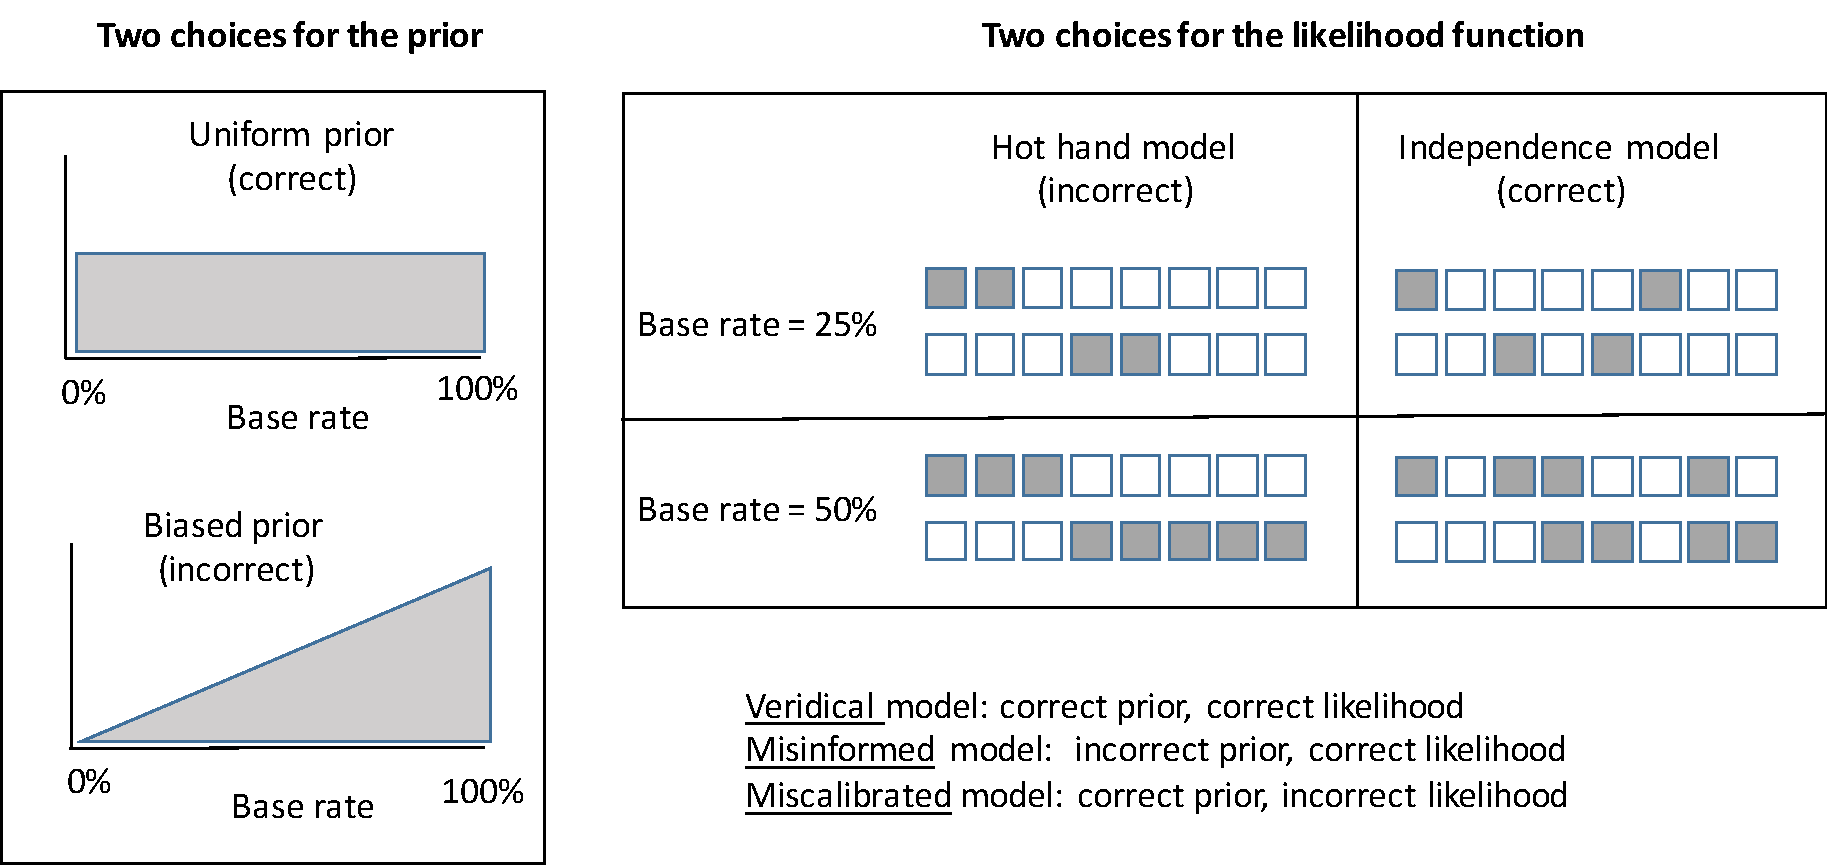
\includegraphics[width=.63\textwidth]{other_figs/threeBayesPic.pdf}}\hspace*{.5cm}
	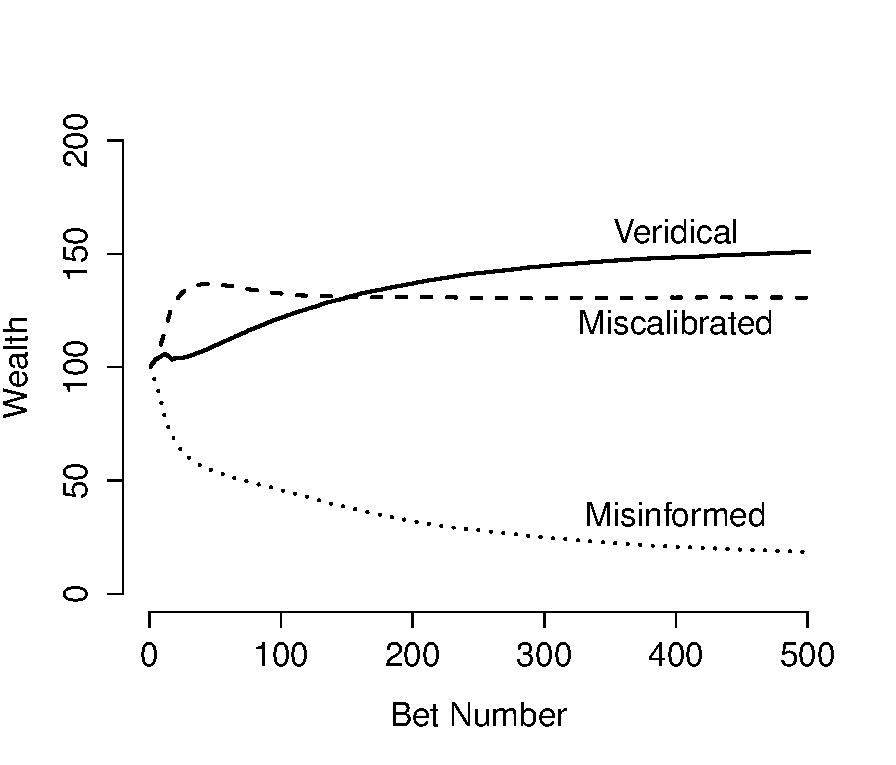
\includegraphics[width=.33\textwidth]{other_figs/threeBayes.pdf}
	\vspace*{6pt}
	\caption{Three Bayesians betting on binary outcomes, where the true success rate $\theta$ is generated randomly from the unit interval. The {\it veridical Bayesian} employs priors and likelihoods that are exactly matched to this task, whereas the {\it misinformed Bayesian} uses the wrong prior and the {\it miscalibrated Bayesian} uses the wrong likelihood. The veridical Bayes outperforms either of the other two models.}
	\label{fig:threeBayes}
	\vspace*{-3mm}
\end{figure}

One of the philosophically appealing features of Dutch book arguments is the fact that this coherence of Bayesian belief revision is an inherent property of Bayes' rule, and not something that is specific to any particular Bayesian model. It is by virtue of this universality that one might argue that all Bayesian models describe a form of rational reasoning, and in one sense it is true. However, it is not at all clear that this kind of rationality is desirable on its own: a Bayesian reasoner whose priors and likelihoods are grossly miscalibrated will find that coherence provides very little protection against losing their money to a better informed agent. In some respects this observation is trite and uninteresting---Teller (1973, p. 224) argues that ``exploitation by dint of such greater knowledge or keener powers of observation shows nothing derogatory about the agent's plan for change of belief.'' In real life, however, few of us would take comfort in such assurances when our incorrect theories about the world lead us to be exploited by others.

As obvious as this point is, we think it ties naturally to the tension that exists in the cognitive science literature. If a Bayesian reasoner applies priors and likelihoods that are well-matched to the world, they are not merely immune to sure losses via a Dutch book, they also enjoy a practical advantage over their less well-calibrated peers in that they are less likely to be exploited by other agents who happen to have better knowledge. This is highlighted in Figure~\ref{fig:threeBayes} which shows the outcomes of a gambling competition between three Bayesian agents. The competition works as follows: a deck of cards consists of black and white cards with some unknown proportion of black cards (the base rate), and cards are turned over one at a time. Each agent offers what they perceive to be fair bets to the others, and each agent places a \$1 stake on any bet they perceive to be favourable. So if an agent believes that the probability of black to be 0.25 they offer 3:1 odds on black, and place a \$1 bet with any agent offering better than 3:1 odds. The true proportion of black cards is chosen uniformly at random at the beginning of the game, and the cards are perfectly shuffled so that outcomes of successive trials are essentially independent. The {\it veridical} Bayesian agent adopts a prior and likelihood that match this scenario perfectly. The {\it misinformed} Bayesian agent uses the correct likelihood (independent events) but incorrectly believes that the scenario has a bias towards black cards. In contrast the {\it miscalibrated} Bayesian agent has the correct prior beliefs about base rates, but incorrectly believes that the deck of cards has not been properly shuffled and thinks that the cards are likely to show a ``hot hand'' effect in which repetitions are much more common than alternation \cite{gilovich_hot_1985}. This set up is illustrated on the left hand side of Figure~\ref{fig:threeBayes}, and the formal details are outlined in Appendix A. On the right hand of Figure~\ref{fig:threeBayes} we plot the results of simulating a large number of gambling competitions among these three agents. Not surprisingly, although all three are Bayesian models -- and hence ``optimal'' in the sense implied by the diachronic Dutch book argument -- they do not perform equally well in these contests. Early on in the gambling contests, the Bayesian models with the correct prior (veridical and miscalibrated) both tend to win money from the misinformed model because it tends to provide overly generous payouts for a bet on white. As the contest continues, the veridical model starts to win money from the miscalibrated model -- because the miscalibrated model incorrectly believes that a hot hand effect applies it offers and places bad bets reflecting its belief that streaks will tend to continue. While each of these three agents represents an optimal solution to some inference problem, only one of them provides a normative standard for gambling behavior in this specific contest. To our mind, good performance on the actual inference problem at hand seems a very important element of what optimality means in the real world, and it is obvious that the mere fact of being Bayesian is not sufficient to guarantee good performance in any satisfactory sense. To be rational, one must do more than just be Bayesian---one must be the right kind of Bayesian.


The point of this discussion to argue that an {\it optimal} Bayesian model is, in practice and for very good reasons, assumed to be something more than just a model with Bayes' rule in it. At the very least, it refers to a Bayesian model in which the priors and likelihoods are well suited to the experimental task or to a real world problem that the agent needs to solve. It suggests that the builders of such models are obligated to constrain their models by making reference to some external standard that justifies the choice of priors and likelihoods.\footnote{Arguably, a Bayesian who wants to make the strongest possible claim about optimality of  {\it cognition} has an even stronger obligation, namely to show that human behavior matches the predictions of the optimal Bayesian model {\it because} that behavior is optimal. This issue is discussed by \citeA{danks_rational_2008}.} For example, the learner's prior might be veridical in the sense of being the correct prior for the task given to participants (as per the toy example above). Alternatively, a prior might be ecologically justified in the sense that it is well matched to the tasks that people have to solve in their everyday lives. These two need not be identical, and if people apply ecologically justifiable priors in an experimental task for which they are not appropriate, one might argue that the cognition is optimally tuned to the real world problem but not the experimental one. The key point is that if one's Bayesian model is intended to be an optimal Bayesian model, the researcher is not free to choose priors and likelihoods purely on the basis of their own intuitions. Indeed, part of the substantive theoretical claim that Bayesian models are often used to make is about the nature of those priors and likelihoods.


\subsection*{Distinguishing optimality claims from descriptive claims}

The idea that human cognition might be optimal or rational is a powerful thought \cite{cosmides_are_1996}, and there seems little disagreement with the suggestion that there would be considerable scientific value to a demonstration that humans closely mimic the behavior of a genuinely optimal Bayesian model, even if that optimality is defined with respect to constraints on factors like sensory abilities or attentional or memory limitations. Much of the excitement about \cite{Griffiths2006,anderson_reflections_1991,kording_bayesian_2004,chater_probabilistic_2006} and criticism of \cite{bowers_bayesian_2012,Mozer2008} Bayesian theories revolves around the plausibility of this vision, but few would argue that the idea would be boring if true. The dispute arises simply because many cognitive scientists strongly disagree with any claim of human optimality \cite<e.g.,>[p. 393]{bowers_bayesian_2012}, noting that in many tasks human performance appears to be markedly suboptimal \cite<see also>[p. 2353]{marcus_how_2013} when compared to a model that makes the best possible inferences given the structure of the task.

Perhaps suprisingly, some recent defences of the Bayesian framework \cite<e.g.,>{griffiths_how_2012,goodman_relevant_2015} against these criticism have been entirely willing to concede that point. If prominent Bayesian cognitive scientists are prompted to argue that ``the hypothesis that people are optimal is not something that even the most fervent Bayesian believes'' \cite[p. 421]{griffiths_how_2012}, why is there so much confusion in the literature surrounding it? A large part of the problem is that the very structure of Bayesian models---because they require the modeller to stipulate and justify the choice of priors and likeilhoods---encourages an optimal interpretation, even on the part of modellers who did not set out with that goal. Indeed, we would suggest that this characteristic that may have given rise to many of the optimality claims that \citeA{bowers_is_2012} highlighted and found so problematic. In contrast, our {\it descriptive} Bayesian models provide a vision that explicitly, as part of its structure, rejects assumptions or interpretations of optimality.

If a particular Bayesian model is not intended to constitute a normative claim about what people should do in order to be deemed rational, what purpose does it serve? In our experience, many researchers who develop Bayesian models are quite uninterested in making normative claims. Instead, the goal is merely use the Bayesian framework as a language in which to specify a theory about the learner's mental representations (hypothesis spaces), the beliefs defined using these representations (the priors), and the learning rules that describe how beliefs are revised (the likelihoods). From this perspective Bayesian cognitive models need not correspond to a strong claim about the optimality or rationality of human behavior. Rather, they serve a descriptive goal based on the conditional claim that {\it if} a learner adopted this prior and that likelihood, {\it then} it would be sensible for them to produce that behavior. Viewed in this way it is still critical that Bayesian models be coherent---and Dutch book arguments are still somewhat pertinent---because without such coherence even this conditional claim becomes untenable. However, a learner's prior need not capture the ``correct'' environmental statistics for some problem nor does it need to be veridical for a specific task; it need only capture {\it some} beliefs that the learner might bring to the task \cite<e.g.,>{Hemmer2014,Huszar2010}. Similarly, a likelihood need not describe the ``true'' model in which observations are generated and might not even map onto a particularly sensible one;
it need only describe how the learner {\it thinks} the observations were generated \cite<e.g.,>{navarro2012}. The hypotheses considered by the learner need not include the {\it best} or most appropriate hypothesis in some objective sense; they need only include some cognitively-plausible set of options a learner might consider. Such a model makes sense on its own terms and serve a useful purpose in illustrating psychological principles, but if the priors or likelihoods are especially mismatched to the task, it is somewhat misleading to refer to such a model as ``rational'' and highly inappropriate to refer to it as ``optimal.''

We refer to models constructed in this fashion as {\it descriptive} Bayesian models.\footnote{Sometimes the term `descriptive' is used to capture models that seek to more clearly characterize data (as in, for instance, signal detection or diffusion models) as opposed to models whose aim is to explain the underlying processes or causal relationships. That is not the distinction we are making here. Rather, we use the term to make the distinction between models that seek to describe the priors and likelihoods people actually use, rather than prescribing them {\it a priori} and justifying them as being well-suited to the problem.} Within the descriptive approach, human cognition need not be perfectly matched to the statistics of the environment, people's learning might not make optimal use of the information inherent in the problem, and individual participants might differ quite substantially in their choice of priors and likelihoods. If human behavior matches the predictions made by a model specified in this manner, this is evidence that the model provides a good description of the behavior---which suggests that the model's assumptions may be consistent the assumptions people make in that situation. Critically, good fit of a descriptive model to human behavior does {\it not} imply that the behavior is rational. It is evaluated and interpreted in much the same way as any other probabilistic model of cognition, on a par with models like signal detection theory \cite{macmillan_detection_2004}, sequential sampling theory \cite{ratcliff_comparison_2004}, multinomial processing trees \cite{batchelder_multinomial_1990}, and so on.

Put another way, the fundamental difference between descriptive Bayesian models and optimal Bayesian models is that within the descriptive Bayesian framework, questions of optimality are simply {\it irrelevant}. This distinction is especially clear when comparing descriptive Bayesian models with models of constrained optimality. The two have sometimes been confused with one another, but they are fundamentally distinct. Models that acknowledge that all optimality occurs within constraints (e.g., investigating whether some behavior is optimal given the existence of certain capacity limitations or filters on the kind of sensory input available) are still optimal models: they still justify the modelling choices by reference to some notion of optimality. That is, the choices of priors, likelihoods, hypotheses, or characteristics are justified by arguing that they are well-matched to the task or in some other way ecologically valid, given the constraints the organism is operating within. A descriptive approach, by contrast, simply doesn't {\it care} whether the choices are justified. The central question of interest is discovering what choices best account for human performance.

This raises the question: if the descriptive approach liberates Bayesian models from the requirement that they be ``rational'' or ``optimal'', why should a researcher adopt such an approach? What are the virtues of Bayesian models if they no longer represent optimal inference or produce rational behavior? It might appear that we are discarding the core virtue of Bayesian models. Yet this is far from the case. Much of the appeal of Bayes' rule lies in the fact that it represents a method for writing down models in a transparent way. To build a Bayesian model, the researcher is forced to specify what form the mental representation might take (the hypothesis space), what biases the learner brings to the problem (the prior), and the rules by which the learner can be influenced by data (the likelihood). Because the researcher cannot write down a Bayesian model without making these things clear, the assumptions of the theory are always out in the open. Such a model tries to explain human behavior in much the same way any other model does: If the learner possesses {\it these} beliefs and reasons in {\it this} way, it would be reasonable to expect them to produce {\it that} behavior.

How, then, are descriptive Bayesian models different from modelling more generally? In one sense they are just one of many options in our toolbox; which approach should be used depends on the research question. But the particular research questions a descriptive approach are well-suited for are exactly the kinds of questions that often arise in cognitive science. What is the nature of the hypotheses people are evaluating when they learn? How exactly do people update their beliefs in response to the data they see, and what assumptions do they make about how that data was generated? What priors do people bring to a learning situation? These questions are more naturally answered within a descriptive framework than an optimal one, and the explicitness of the Bayesian machinery means that for those kinds of questions it can offers advantages of explicitness and precision over other modelling frameworks as well.



\subsection*{A formal statement of the descriptive Bayesian approach}

Relaxing the requirement that Bayesian models describe optimal cognition opens up the possibilities for investigation considerably. In an optimal Bayesian model, the learner's inferences are described via the application of Bayes' rule:
\be
P(h|x) = \frac{P(x|h)P(h|\mathcal{H})}{\sum_{h^\prime \in \mathcal{H}} P(x|h^\prime)P(h^\prime|\mathcal{H})}
\label{eq:obmc}
\ee
where $x$ represents the data available to the learner, $h$ is a hypothesis about the origins of the data, and $\mathcal{H}$ represents the set of hypotheses available to the learner. In order to satisfy some version of the optimality claim, the priors and likelihoods need to be constrained in an a priori fashion.

The descriptive view rejects the idea that priors and likelihoods should be constrained by anything beyond the researcher's theory of the task. The learner's prior should not be viewed as fixed by the structure of the environment, nor should it necessarily correspond to a sensible expectation about the world. Similarly, the likelihoods that govern people's learning need not correspond to any realistic model of how observations are generated. As such, the behavior produced by the model need not be rational or even particularly sensible. Formally, if there are multiple possible choices of prior (parameterized by $\phi$) and likelihoods (parameterized by $\lambda$), then the learner's inferences are conditioned on these parameters:
\be
P(h|x,\lambda,\phi) = \frac{ P(x|h,\lambda) P(h | \phi, \mathcal{H}) }{\sum_{h^\prime \in \mathcal{H}} P(x|h^\prime, \lambda) P(h^\prime|\phi, \mathcal{H})}
\label{eq:ddbmc}
\ee
In one sense the difference between these two expressions is purely cosmetic: Equation~\ref{eq:obmc} suppresses the dependence on the parameters $\phi$ and $\lambda$, whereas Equation~\ref{eq:ddbmc} makes the dependence explicit. However, this distinction is central to the manner in which a descriptive Bayesian model differs from a traditional rational analysis. If the purpose of a Bayesian model is to make claims about optimality, the parameters $\phi$ and $\lambda$ are nuisance variables that (ideally) should be fixed by reference to some external standard. However, if the purpose of a Bayesian model is to help us develop good descriptions of human cognition, the core goal is now to {\it learn} what priors and likelihoods people rely on. Inferring the priors $\phi$ and likelihoods $\lambda$ from the empirical data is now the aim.\footnote{It should be noted that this is a slight oversimplification. For instance, in some situations (e.g., our case study 3) the goal is to infer the {\it hypothesis space} $\mathcal{H}$. The notation could be expanded to express this but for expositional simplicity we suppress this for now.}

W can illustrate the difference between a descriptive and optimal model with a simple category learning example. If the researcher is operating within an optimal Bayesian framework, when they specify their model they should consider what kinds of category-learning priors would be optimal: for instance, they might incorporate a prior that favors more coherent categories \cite{rosch78} on the grounds that such a category system is sensible \cite{navarro_hypothesis_2011}. They should also consider what kinds of likelihood models an optimal learner should entertain: perhaps one that assumes strong sampling and follows the size principle on the grounds that it is statistically appropriate if one assumes that data is drawn directly from the category itself \cite{Tenenbaum2001}. The key point is that an optimal Bayesian modeller needs to not only make choices about the prior and likelihood, but they should be able to justify those choices as optimal for some reason. By contrast, a descriptive Bayesian modeler need not do this. Instead, they perform inference {\it over} the priors and likelihoods\footnote{As we describe in more detail below, it is of course impossible to perform inference without setting some hyper-prior on the priors and likelihoods themselves. Yet these hyper-priors can be loose enough to permit a large range of variation in the actual priors and likelihoods entertained by the model. As such, they themselves need to be justified on optimality grounds, and they allow the researcher to truly do inference about which parameters best describe human performance} of each participant and discover which ones best account for their performance. Perhaps some people use strong sampling, while others do not; perhaps everybody, or nobody, or a few people do not have particularly strong {\it a priori} beliefs about the coherence of categories. The descriptive approach allows researchers to discover this.

The descriptive approach to Bayesian cognitive modeling allows the researcher a lot of freedom in how the model can be built and parameterized, so it becomes critical to consider how the model parameters should be estimated and how rival models should be compared. Fortunately, these are well-studied problems and many principled solutions exist for model selection   \cite<see e.g.,>{browne_cross-validation_2000, pitt_global_2006, pitt_toward_2002, myung_importance_2000, myung_model_2006, wasserman2000bayesian, Shiffrin2016, ShiffrinInPress, ChandramouliInPress}, and perhaps the most elegant approach to parameter estimation is Bayesian data analysis \cite<e.g.,>{lee_bayesian_2014, kruschke_doing_2010, gelman_bayesian_2014}, in which the {\it researcher} also acts as a Bayesian reasoner. Before running any experiment, the researcher themselves has some priors $P(\lambda,\phi)$ that captures their beliefs about which priors and which likelihoods are plausible. After running the experiment she obtains a collection of responses $r$ from the participant, from which she infers a posterior distribution $P(\lambda,\phi|r)$. This distribution captures everything the researcher has learned about the participant using her model and the data from her experiment. The inference by the researcher can also be described using Bayes' rule,
\be
P(\lambda,\phi | r) = \frac{P(r|x,\lambda,\phi)P(\lambda,\phi)}{\int P( r| x,\lambda^\prime,\phi^\prime) P(\lambda^\prime,\phi^\prime) \ d(\phi^\prime, \lambda^\prime)}
\ee
In this expression, we use the notation $P(r | x,\lambda,\phi)$ to indicate that the participant responses $r$ depend on both the parameters $(\lambda,\phi)$, and on the information $x$ that the experiment presents to the participant. In order to do so, the researcher needs to specify two things. Firstly, as noted above, she needs to specify the prior distribution over model parameters, $P(\lambda,\phi)$. Secondly, she needs to specify a data analysis model that links the learner's posterior distribution over hypotheses $P(h|x,\lambda,\phi)$ to the researcher's likelihood function for the data, $P(r | x,\lambda,\phi)$. Specifying the data analysis model requires the researcher to make substantive choices. For instance, one might assume that people generate their response by sampling from the posterior \cite<e.g.>{vul_one_2014}, but other possibilities exist. Several simple possibilities are listed by \citeA{marcus_how_2013}, but there is no reason why a complex theory of the response generation process could not be supplied \cite<see e.g., the Appendix in>{navarro2012}. The important point is that if the researcher does specify a clear measurement model that links the learner's posterior $P(h|x)$ to the observed responses $r$, then all of the statistical machinery of Bayesian data analysis and other approaches to model selection now become available.


\subsection*{Summary}

The descriptive approach to Bayesian cognitive modeling has many fundamental differences from a view in which Bayesian models are treated as optimal, normative standards for human cognition. Firstly, the descriptive approach treats the cognitive model as a {\it tool} to make inferences about participants. When building a model, the researcher is not obligated to have a theory that precisely states what priors and likelihoods a learner should use. Instead, they can propose a broad family of possible Bayesian models and use the experimental data to infer which of those models best matches human behavior. Secondly, it provides a natural mechanism for expressing individual differences, as it allows each participant to have different priors $\phi$ and likelihoods $\lambda$ without obligating the researcher to suppose that each person's idiosyncratic prior and likelihood is fully justified given their idiosyncratic experiences. Thirdly, because the descriptive framework emphasizes the importance of treating the Bayesian cognitive model as a genuine statistical model for the data (i.e., ideally, it assigns probabilities to people's responses at a trial to trial level), we can use a number of model selection approaches, including methods from Bayesian statistics, to compare between models of different sorts (even if some of those models are non-Bayesian).

The primary goal in this paper is to highlight the importance of making a clear {\it distinction} between an optimal Bayesian model and a descriptive one, and the rest of the paper is devoted to illustrating why this distinction matters. To that end we present three case studies. Our first case study presents an example in which an optimal Bayesian model fails to account for human behavior, whereas a descriptive Bayesian model performs better---by dropping the presumption of optimality and allowing for individual differences---and yields novel insights into how people solve a simple inductive problem. The second case study presents an example in which the comparison between an optimal Bayesian model, a descriptive Bayesian model, and a non-Bayesian model explores how close people actually are to optimal in some cases. This case study illustrates that even when people's behavior is {\it actually} close to optimal, the descriptive framework is still useful. Not only does it provide a framework for making the  comparison, but it also constitutes {\it better} evidence for optimality than an optimal model alone would: the priors and likelihoods that correspond to the normative solution are rigorously shown to provide the best account of the data, rather than being simply stipulated by the modeller. Finally, our third case study highlights the fact that descriptive Bayesian models can still be useful in situations where exploring whether or not people are optimal is irrelevant to the research question.

These examples are intended to be illustrative, not exhaustive. We aim to highlight the potential power of the descriptive approach, not to catalog all possible uses of the framework. Although there are a number of important technical details to consider when applying Bayesian data analysis to a Bayesian cognitive model, we have aimed to keep these technical details to a minimum in the main paper, but more fully elaborated in the Appendices. Finally, we should note that although our examples are chosen to illustrate why it can be useful to build descriptive Bayesian models, we believe that there is a place for both kinds of Bayesian models in the literature. For instance, optimal Bayesian models are quite appropriate in cases where the modeller has independent substantive justification for the choice of likelihoods and priors; in such a situation, the extra machinery of the descriptive approach may be unnecessary.


\section{Case study 1: Focusing on optimality does not always lead to the best understanding of human behavior}

Our first case study revisits the Bayesian theory of coincidences and discoveries developed by \citeA[henceforth GT1]{Griffiths2007}. The central goal in that paper was to develop a Bayesian account of how people decide whether a pattern of observations is a mere coincidence (a chance occurrence) and when it represents a meaningful discovery. The paper uses Bayesian models to make normative claims. For instance, the abstract of the paper argues ``that people can {\it accurately} assess the strength of coincidences, suggesting that {\it irrational conclusions} drawn from coincidences are the consequence of overestimation of the plausibility of novel causal forces'', and on page 218 the authors argue that  ``human {\it irrationality} concerning coincidences [can] be localized in miscalibrated prior odds'' (emphasis ours). The normative claims are clear: To agree with this model is to be accurate and rational, and disagreements with the model are irrational. Moreover, to the extent that discussion of the Bayesian theory focuses on such claims, the purpose of constructing the Bayesian model appears to be that it licenses these normative claims.

In this case study we focus on two problems that sometimes arise when applying the optimal Bayesian approach. First, demonstrating that aggregated response curves match those produced by an optimal model may not provide sufficient evidence that people's behavior is optimal if {\it individual} responses deviate from the optimal norm. Second, when behavior cannot reasonably be considered to be optimal, this type of model loses its explanatory power and provides limited psychological insights. We address these issues by including a descriptive Bayesian model in our analysis---one that best describes human behavior and drops any normative claims about the rationality of human cognition---and show that this leads to additional insights about human psychology, including a more nuanced understanding of how people's behavior deviates from optimality.


\subsection{Of genetics and psychokinetics: Inference from binary data}

The original GT1 paper discusses several different inference problems and develops a Bayesian model for each one, but for our purposes it will be sufficient to consider the simplest case. In their first experiment, they presented people with descriptions of fictitious scientific experiments in which the observed outcomes were binary, and the question people had to answer was whether the true base rate of the outcomes was 50\%. There were two versions of the task. People in the {\sc genetics} condition were given the following cover story:

\begin{quote}
{\it A group of scientists investigating genetic engineering have conducted a series of experiments testing drugs that influence the development of rat fetuses. All of these drugs are supposed to affect the sex chromosome: they are intended to affect whether rats are born male or female. The scientists tested this claim by producing 100 baby rats from mothers treated with the drugs. Under normal circumstances, male and female rats are equally likely to be born. The results of these experiments are shown below: The identities of the drugs are concealed with numbers, but you are given the number of times male or female rats were produced by mothers treated with each drug.}
\end{quote}

\noindent
After being told that (say) 70 out of the 100 baby rats were male, participants were asked to assess the probability that the drug was effective. In a classical null hypothesis test, the inferences that one makes in this scenario depend only on the raw data (i.e., number of males and number of females). However, GT1 argue that people should treat this as Bayesian inference problem and use the cover story to impose some prior bias. To that end, a second group of participants (in the {\sc psychokinesis} condition) saw this cover story:

\begin{quote}
{\it A group of scientists investigating paranormal phenomena have conducted a series of experiments testing people who claim to possess psychic powers. All of these people say that they have psychokinetic abilities: They believe that they can influence the outcome of a coin toss. The scientists tested this claim by flipping a fair coin 100 times in front of each person as they focus their psychic energies. Under normal circumstances, a fair coin produces heads and tails with equal probability. The results of these experiments are shown below: The identities of the people are concealed with subject numbers, but you are given the number of times the coin came up heads or tails while that person was focusing their psychic energies.}
\end{quote}

Participants were then shown the outcomes of a series of these experiments---the number of male rats or the number of heads out 100 trials---and had to judge the probability that the drug affected the sex of rats, or that the person had psychic powers. In order examine how people's beliefs are the strength of evidence in the data, they asked people to judge the probability that the drug/psychokinesis was effective in 8 different situations: when the number of males/heads was 47, 51, 55, 59, 63, 70, 87, 99 and 100.


\subsection*{An optimal Bayesian model}

How should an optimal reasoner behave when solving this problem? GT1 present the following rational analysis of the task. There are two hypotheses that need to be discriminated: According to the ``null'' hypothesis $h_0$, the true probability of male/heads is fixed at 50\%, but according to the ``alternative'' hypothesis $h_1$ the true probability is an unknown value $\theta$ that could be anywhere between 0 and 1. This framing of the problem seems entirely reasonable and in fact this exact model is sometimes used as a simple data analysis tool \cite<e.g.,>{wagenmakers_practical_2007}. Formally, if $n$ denotes the number of observations and $k$ denotes the number of successes, then the strength of evidence provided by the data is provided by the Bayes factor:
\begin{equation}\label{eq:gt1-likelihood}
\dfrac{P(\bm{x} \mid h_1)}{P(\bm{x} \mid h_0)} = \dfrac{2^n}{\tbinom{n}{k}(n+1)}
\end{equation}
The further that the proportion $k/n$ deviates from 0.5, the stronger the evidence for the alternative model. However, there are good reasons to think that people would be more skeptical of a claim about psychic powers than a claim about genetic engineering, and so GT1 argue that people should employ different priors in the two conditions. This also seems sensible, and similar claims about the importance of adapting the prior to suite the problem have been made in the Bayesian data analysis literature \cite{wagenmakers_why_2011}. Multiplying the Bayes factor by the prior odds $P(h_1)/P(h_0)$ gives us the posterior odds ratio,
\begin{equation}\label{eq:gt1-posterior}
\dfrac{P(h_1 \mid \bm{x})}{P(h_0  \mid \bm{x})} = \dfrac{P(\bm{x} \mid h_1)}{P(\bm{x} \mid h_0)} \times \dfrac{P(h_1)}{P(h_0)}
\end{equation}
which reflects the relative strength of belief that the learner has in the two hypotheses after the data have been observed.

The optimal model developed by GT1 is elegant, simple and makes very clear predictions about how different experimental manipulations should change people's judgments. The cover story manipulation should shape people's priors $P(h)$, the number of observed cases should affect the likelihood $P(x|h)$, and these two factors should be integrated via Bayes' rule. In light of the way in which they constructed their task and presented it to participants, we would strongly agree with their claim that this model does make sense as a normative standard for this task.

\subsection*{Successes and failures of the optimal model: A replication of the GT1 study}

How plausible is the claim that people are optimal at this task? To evaluate the optimal Bayesian model as a theory of human behavior, we conducted a replication of the GT1 experiment using 102 participants recruited through Amazon Mechanical Turk. Participants were paid \$0.40 for completing the study. The only difference between our study and the original one is that we used a slightly different dependent measure: We asked people to judge the probability that a real effect was observed. Following GT1, we excluded participants who appeared to have reversed the response scale (i.e., showed decreasing confidence in an effect as $k$ increased), leaving 89 participants. The results of the original study and our replication are shown as the solid lines in in Figure~\ref{fig:aggregate}. As is immediately clear from inspection of the figure, the empirical result from GT1 replicates.

\begin{figure}[!t]
	\centering
	(a) \\
	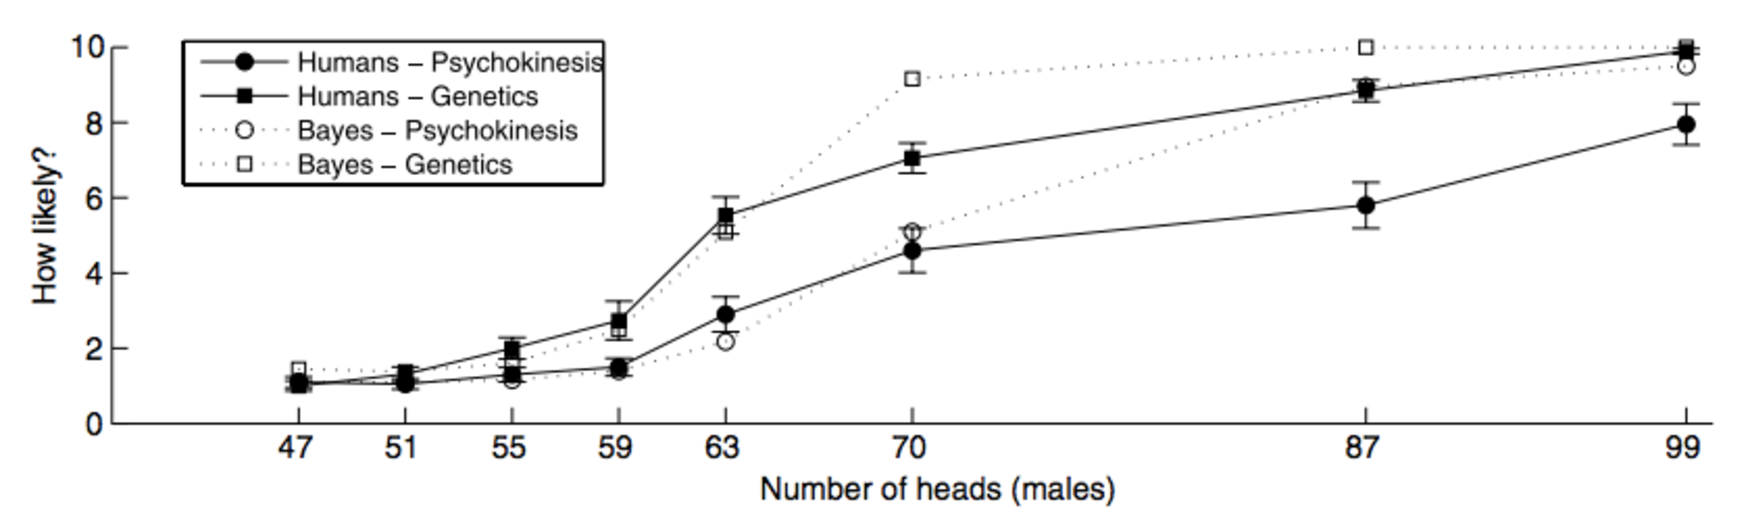
\includegraphics[width=0.7\textwidth]{coincidences_figures/gt1aggregate.pdf} \\
	(b) \\
	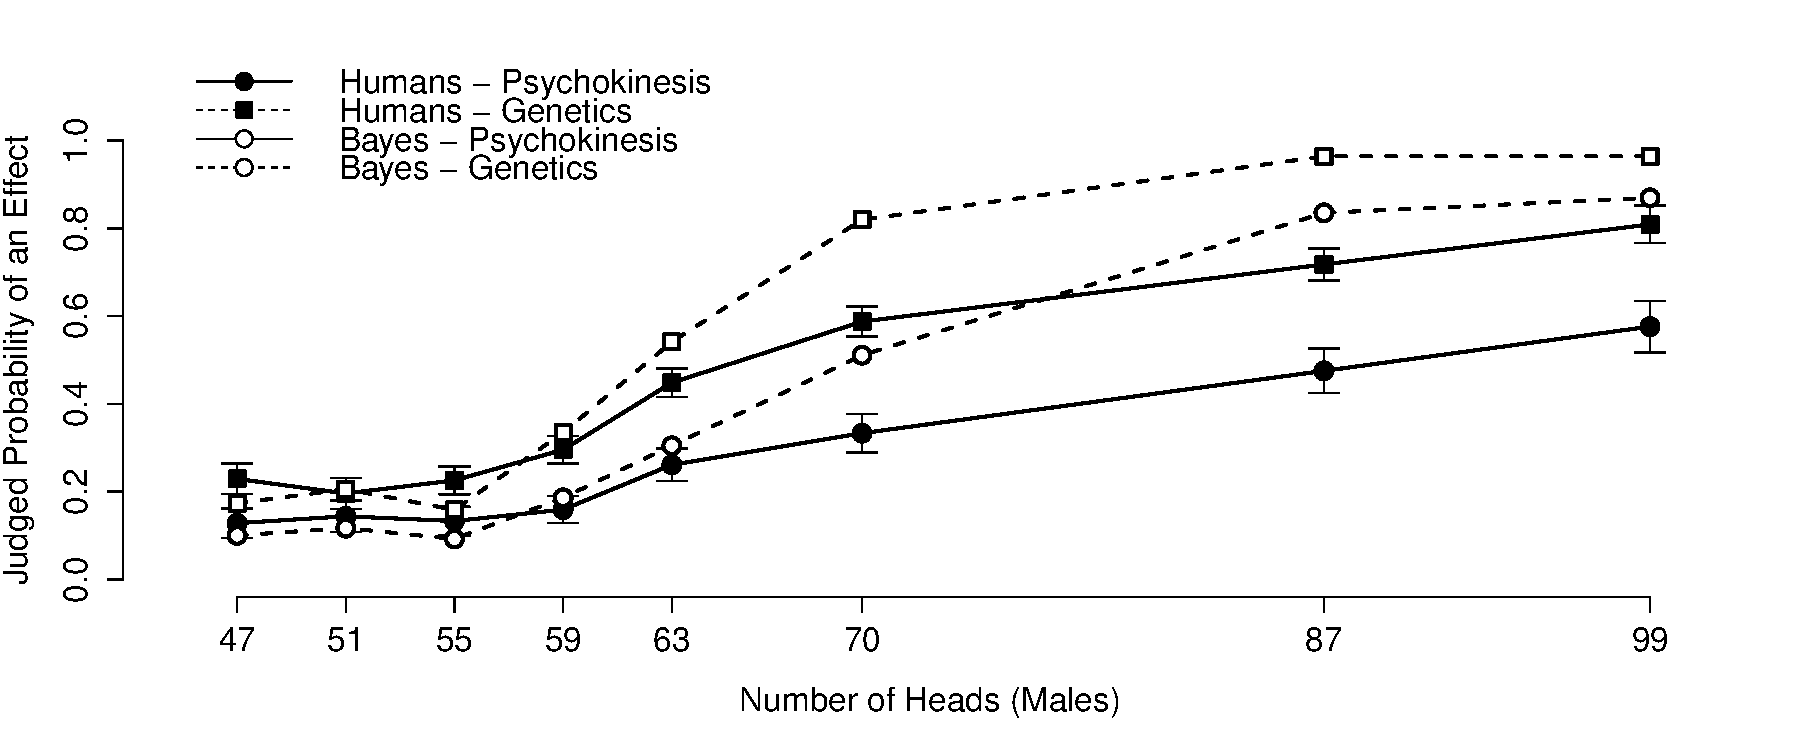
\includegraphics[width=0.75\textwidth]{coincidences_figures/usaggregate.pdf} \\
	\caption{Aggregated fits of the original Bayesian coincidences model. Panel (a) is a reproduction of Figure 3 from \protect\citeA{Griffiths2007}, whereas panel (b) shows the results from our replication of the experiment and model fitting procedure from the original paper. Error bars in panel (b) are standard errors. While there are some differences between the two panels, and some disagreements between the Bayesian model and human performance, the overall qualitative agreement is reasonable.}
	\label{fig:aggregate}
\end{figure}

In addition to replicating the experiment itself, we replicated the data analysis reported by GT1. When considering the application of the optimal model to empirical data, GT1 quite sensibly acknowledge that their Bayesian model allows room for some individual differences. As they note, it is reasonable to think that different people could read the same cover story and apply somewhat different priors. To accommodate this, they estimate a single free parameter (the prior odds) for each participant, and then reported the averaged responses for both model and humans.\footnote{A minor point on the model fitting exercise: the GT1 paper does not state what procedure was used to estimate parameters, though when fitting the data from our replication we found that minimizing sum squared error worked well. There is also a slight ambiguity in the way in which GT1 describe their procedure, insofar as the text refers to ``fitting the sigmoid function'' (their Equation 6), but also state that the parameters of the relevant sigmoid were fixed to have gain 1 and bias 0. On our reading of the text, it appears that this is intended to mean that the only free parameter in the model is the prior $P(h_1$), and that the sigmoid referred to in the relevant passage is intended only to ensure that $P(\mbox{effect}|\bm{x}) = P(h_1 | \bm{x})$.} These aggregated curves are plotted in Figure~\ref{fig:aggregate} and it is again clear that our replication of the data analysis is in agreement with the results in GT1. In both figures it is clear that the averaged model fits are a reasonable approximation to the averaged data, though clearly there are some fairly noticeable deviations too.

\subsection{A closer look at the individual differences}

Figure~\ref{fig:aggregate} presents a single clean picture, one in which there is one pattern of performance produced by humans, and another single pattern produced by an optimal Bayesian reasoner. The fact that these two curves are in agreement (at least qualitatively) does make it look like people are doing optimal inference. Yet one is compelled to wonder: Do the responses of individual subjects look anything like these aggregated curves? Do individual subjects rely on a likelihood function based on independent Bernoulli trials? Should we call their reasoning be ``irrational'' if they do not?

Viewed in this fashion, it is difficult to assess GT1's proposal that people behave optimally with respect to their prior: Their analysis acknowledges that individual differences might exist and estimates model parameters at the individual subject level, yet ultimately the model performance is assessed only in terms of the aggregated data.\footnote{We do not intend to single out these particular authors on this point. Averaging is a common practice that has often been criticized in the data analysis literature \cite<e.g.,>{Lee2005,Navarro2006}, and there are many well-documented examples in which averaging systematically distorts the structure of the data \cite<e.g.,>{estes_problem_1956,heathcote_power_2000}. It is not a failing unique to Bayesian cognitive models.} In light of these concerns, Figure~\ref{fig:nonoptimal} plots the responses at an individual subject level (right panel), and contrasts these individual subject curves with the response curves produced by the optimal Bayesian model under different choices of the prior odds parameter (left panel). As is immediately obvious from inspection, there is a major mismatch between the two. The curves produced by the Bayesian model are extremely steep,\footnote{It is worth noting that the shallower curves produced by the model at an aggregate level (i.e. in Figure~\protect\ref{fig:aggregate}) are purely an averaging artifact. The original Bayesian analysis reported by GT1 {\it cannot} produce shallow response curves for individual subjects.} whereas almost all the empirical curves are quite shallow. Even before attempting to quantify model performance (see below), it is clear the optimal Bayesian model does not provide a good account of human behavior at an individual subject level. Absent any evidence that human behavior matches the model predictions, it is difficult to substantiate any claim about the optimality of human performance in this task. On the contrary, when measured against the standard that GT1 proposed---optimal belief revision with respect to a prior that can vary from person to person---human cognition appears to be decidely suboptimal.


\begin{figure}[t]
	\centering
	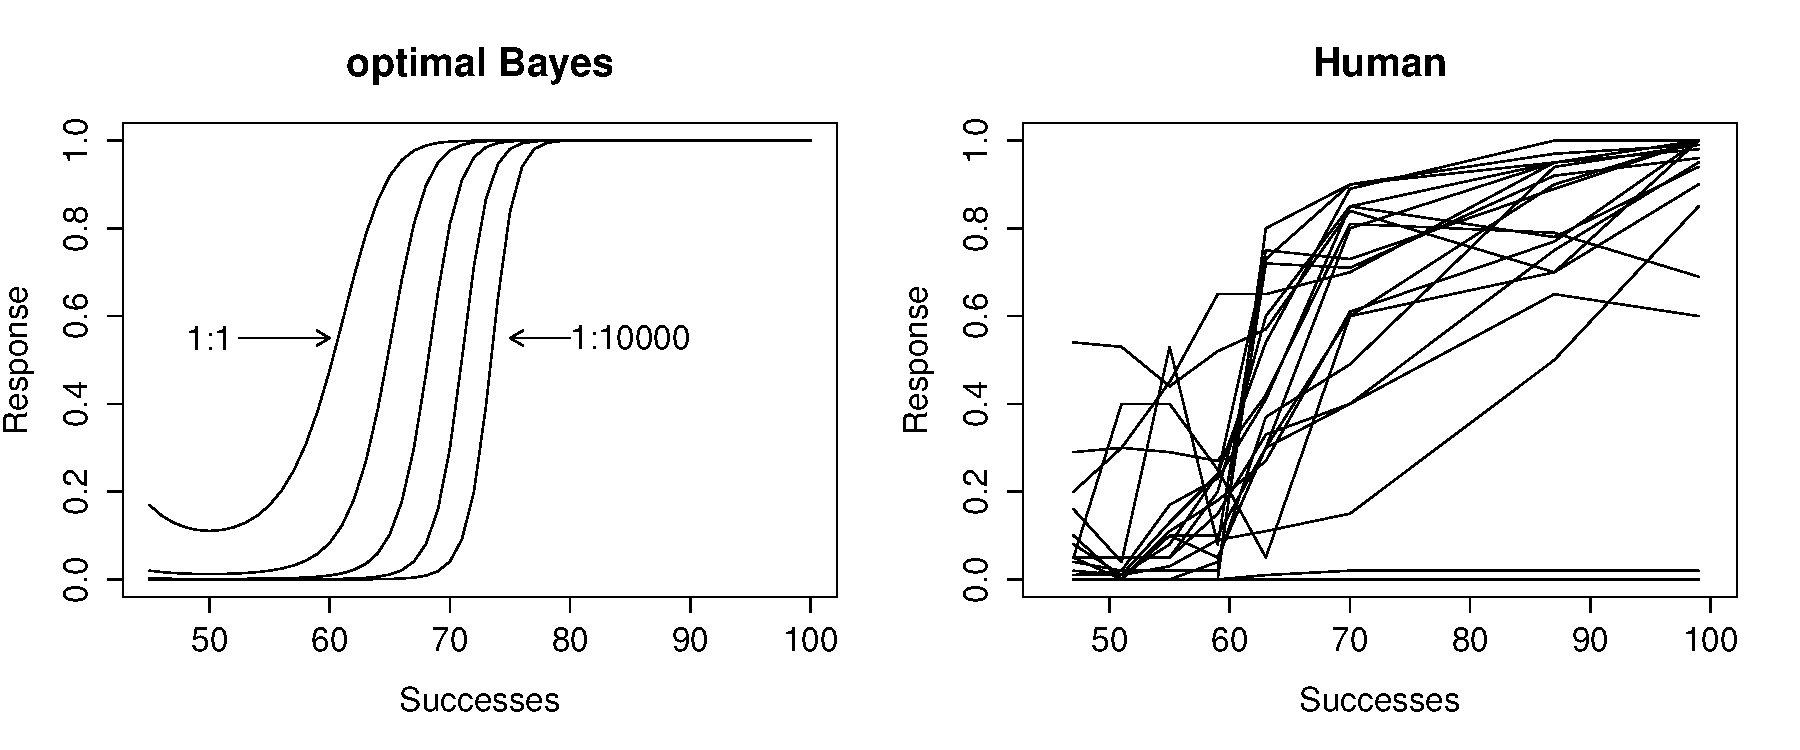
\includegraphics[width=1\textwidth]{coincidences_figures/nonoptimal.pdf}
	\caption{Systematic failures of the optimal Bayesian model for the coincidences task. The left panel plots the response curves predicted by the Bayesian model across a range of possible prior odds. For all choices of priors, the response curves are {\it extremely} steep, much moreso than the averaged curves plotted in Figure~\protect\ref{fig:aggregate}. In contrast, the right panel shows the response curves produced by 20 individual subjects, almost all of which are much shallower. }
	\label{fig:nonoptimal}
\end{figure}



\subsection*{A descriptive approach to the problem}

Given that the normative model proposed by GT1 does not provide a good account of the data, one might be tempted to conclude that we have exhausted the value of Bayesian cognitive models of this problem. Having shown that human performance is not optimal, perhaps we are now obligated to discard the Bayesian approach and turn to non-Bayesian accounts of human performance? We argue that this need not be true. In this section we present a descriptive Bayesian account of the same inference problem, and show that this approach sheds light on human performance even though we cannot use this model to justify any claim that the behavior it describes is rational, optimal or even appropriate.

To construct our model, we begin by dropping GT1s claim that people integrate prior knowledge and statistical evidence in an ``appropriate'' fashion. Instead of requiring that our model use the Bernoulli likelihood function that a statistician might use to analyze scientific experiments, we allow specify a broad family of likelihood functions and seek to {\it learn} which ones produce human-like behavior. These likelihood functions may be appropriate to some real world problem that people have to solve, or they may not. Our initial goal is exploratory: Instead of using the Bayesian analysis as a tool to make claims about the optimality or appropriateness of people's responses, we treat it as a descriptive tool that helps us interpret the experimental data. From this descriptive perspective, it seems natural to want to explore the nature of individual differences and give them more prominence in the data analysis.

With these goals in mind, we extend the model from GT1 in the following ways. Like GT1, we assume that people might have different priors. Letting $\phi = \log P(h_1)/P(h_0)$ denote the prior log odds, we approach the statistical inference problem as Bayesian data analysts and place a prior over $\phi$. More importantly, since we are giving up on the claim that people are necessarily adhering to an easily-definable standard of ``optimality'', we can take line of reasoning one step further. Why should people differ in their priors but not also their likelihoods? Assuming that everyone has the same likelihood function, as expressed in Equation~\ref{eq:gt1-likelihood}, makes sense if all people update their beliefs ``optimally'' (i.e., based on the assumption that each observation is the result of an independent Bernoulli trial). This is indeed what statistical models for binary data typically assume, but that does not mean that people make the same assumption. In many tasks people appear to update their beliefs conservatively \cite{phillips_conservatism_1966}, increasing their confidence in a proposition more slowly than the statistical evidence would warrant.

Incorporating conservatism into the GT1 model is not technically difficult. For example, a simple way to behave conservatively in this task is for the learner to apply Equation~\ref{eq:gt1-likelihood} to a smaller ``effective'' sample size than the one actually observed. Formally, we let $\theta$ denote the effective value of a single datum (ranging from 0 to 1), where each value of $\theta$ corresponds to a different likelihood function, and we obtain the original model from GT1 when $\theta=1$ \cite<see also>{navarro2012,RansomINPRESS}. Then, in the same way that we assume that people can have different priors $\phi$, we allow the possibility that each person has their own likelihood function defined by $\theta$. Then, adopting a Bayesian data analysis perspective, we as researchers specify our priors over the model parameters $\phi$ and $\theta$ and allow the empirical data to teach us something about our participants (see Appendix A for details).

An important point to recognize is that while our expanded model is clearly {\it Bayesian}, it is difficult to characterize as an {\it optimal} model for the task that people were asked to solve. If participants do turn out to be conservative in their inferences, for intance, it is not at all obvious whether this conservatism has any normative justification. It is of course possible to construct post hoc stories about why it might be justified: One might argue that real world data are messy and autocorrelated, and as such it would be rational to display some conservatism if people transfer those expectations to the GT1 task. But even if this explanation were correct how much conservatism would real world messiness justify? It is not clear that there is a unique solution to this question. If our scientific goal is to judge whether people are doing the ``right thing'' or the ``wrong thing'', adding conservatism to the model seems to do nothing but muddy the waters. On the other hand, if we adopt the more exploratory goal of trying to find the statistical model that best describes human behavior, the focus shifts to empirical questions. What likelihoods and priors produce human-like behavior? Do they differ from person to person? Do they differ from context to context? These are questions we can investigate within the descriptive Bayesian framework, using the model as a tool, without being obligated to endorse any claim that the behavior that the model describes is optimal in any interesting sense of the word.

\begin{figure}[p]
	\centering
	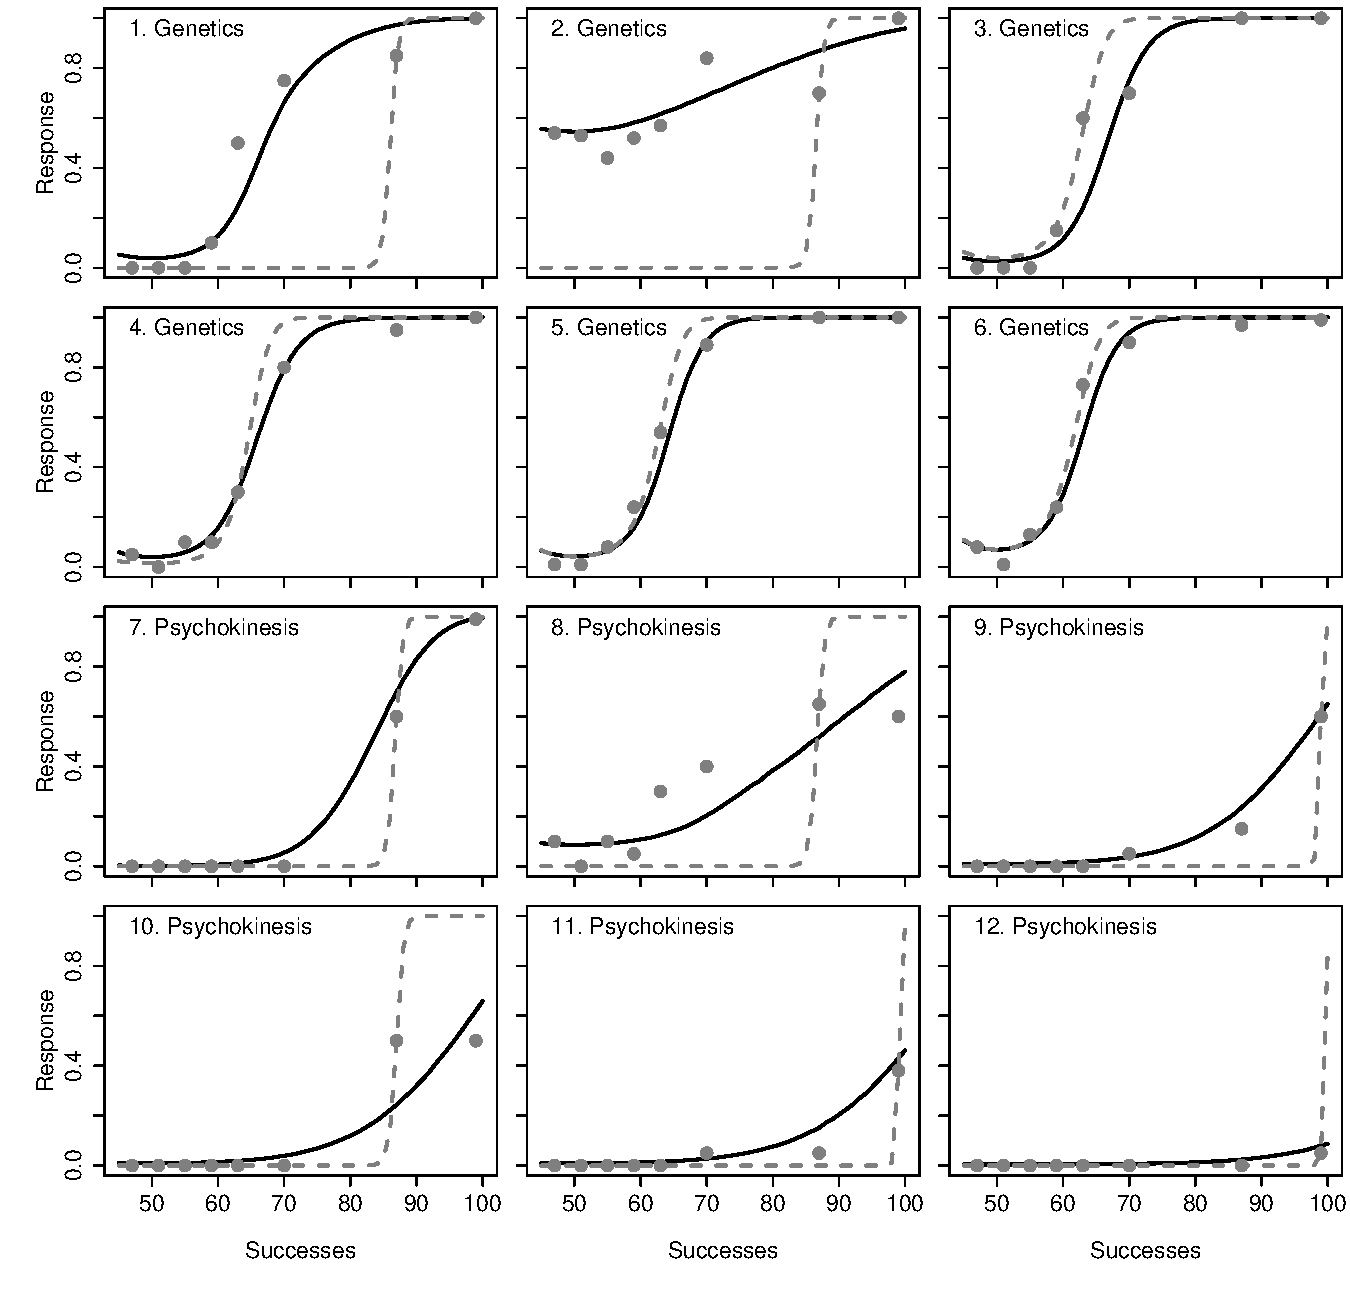
\includegraphics[width=1\textwidth]{coincidences_figures/individuals.pdf}
	\caption{Individual differences in the coincidences task. Each panel plots the responses from a single participant (dots). The top six panels show participants assigned to the {\sc genetics} condition and the bottom six panels show participants in the {\sc psychokinesis} condition.
Solid lines show the posterior predictive mean for the descriptive Bayesian model. Dotted lines show the fitted values for the original, optimal Bayesian model. It is clear that while the original model produces reasonable fits in some cases, in others (e.g., panels 1, 2, 8, 9, and 10) it performs much more poorly than the descriptive model. This is because it does not allow for any flexibility in the likelihood function, predicting a very steep rise as a function of the input.}
	\label{fig:indiv}
\end{figure}


\subsection*{Results}

\subsubsection*{The descriptive Bayesian model captures individual response curves}

Figure~\ref{fig:indiv} plots the raw data for twelve participants. In these plots, the dashed line shows the best fitting response curves for the original Bayesian model proposed by GT1, and the solid lines show the curves produced by the descriptive model. As is evident from inspection, there are some subjects who produce response curves that are in close agreement with the optimal Bayesian model. However, it is also evident that the optimal model only captures one possible human-like response pattern. In contrast, our expanded model provides reasonably good fits to all participants shown in Figure~\ref{fig:indiv}. For those participants who produce steep response curves, our model agrees with the original GT1 model. But the descriptive model can capture the behavior of people who produce shallower curves. As a result, by virtue of allowing a wider range of likelihood functions, our model passes a basic test of descriptive adequacy that the GT1 model fails. This is reflected in the average sum squared error between the model fits and the human data at the individual subject level: For the GT1 model it was 0.41 (sd = 0.45), whereas for the descriptive model it was 0.10 (sd = 0.14).

\bigskip

\begin{figure}[]
	\centering
	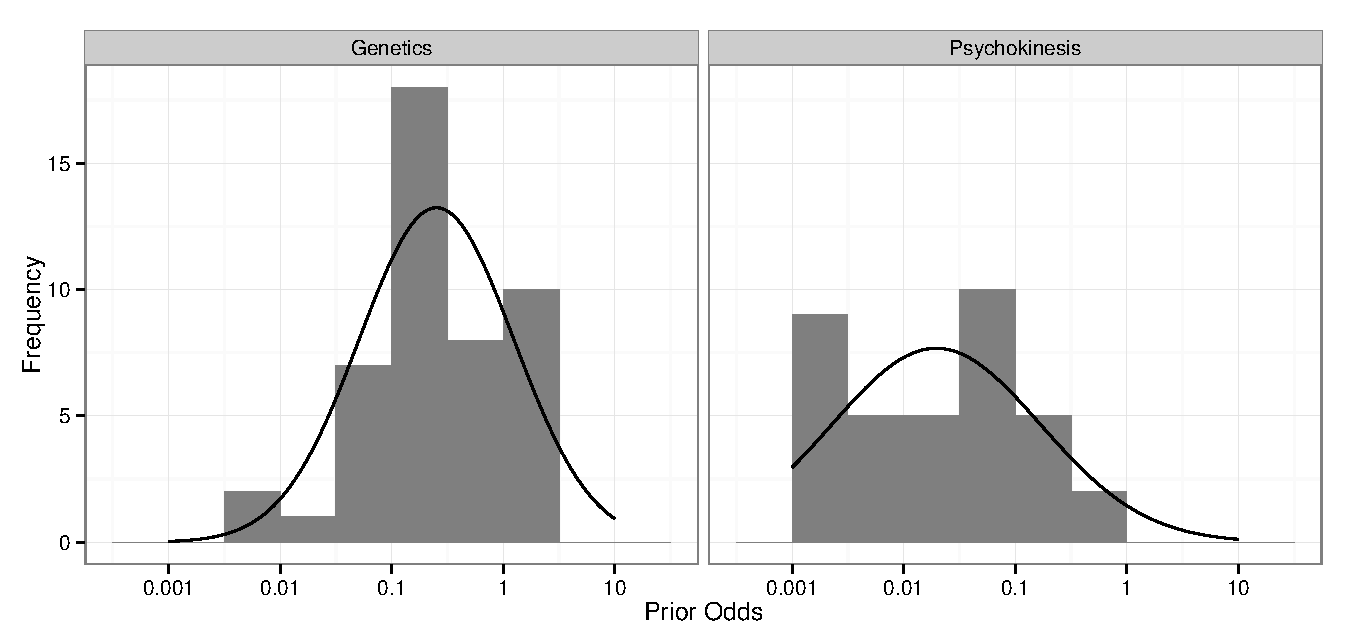
\includegraphics[width=.95\textwidth]{coincidences_figures/priorVariation.pdf}
	\caption{The cover story has a strong influence on the prior probability of an effect. Individual subject distributions over the prior odds vary with condition, with people who saw the {\sc genetics} cover story giving much higher prior odds of a real effect. Even within condition, however, people vary a great deal in their prior beliefs.}
	\label{fig:coverstory}
\end{figure}

\begin{figure}[]
	\centering
	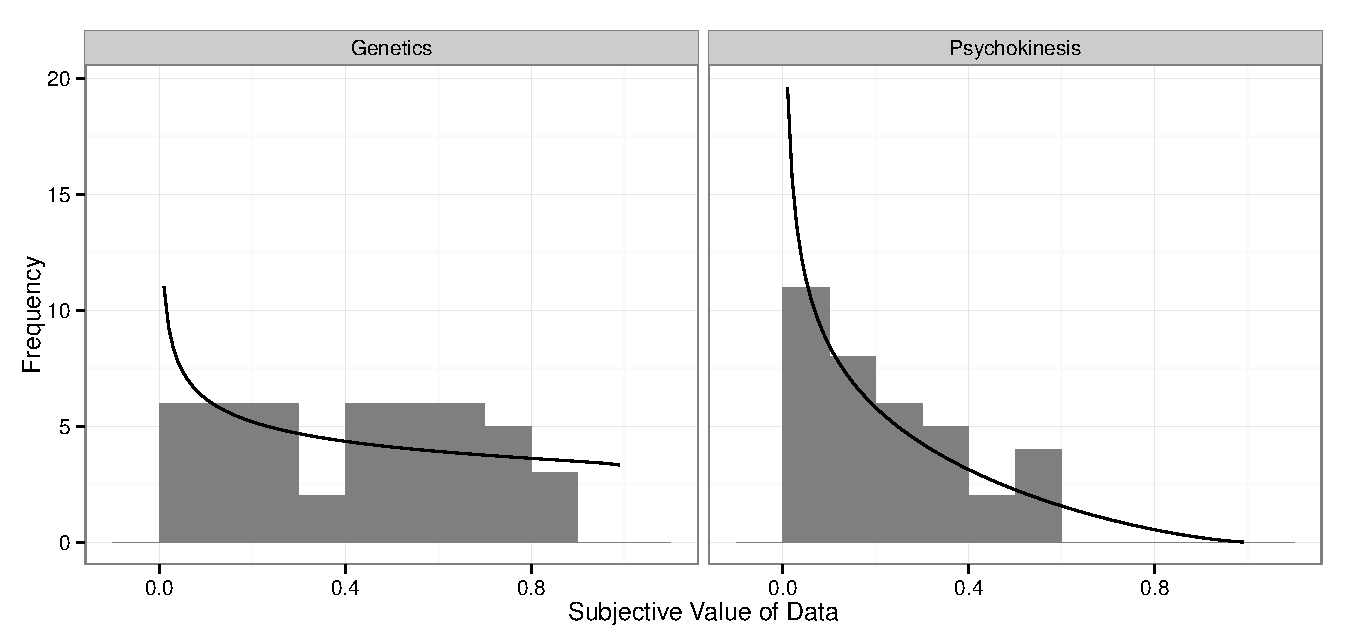
\includegraphics[width=.95\textwidth]{coincidences_figures/likelihoodVariation.pdf}
	\caption{The cover story has an influence on the likelihood. Individual subject distributions over the likelihood also vary with condition, suggesting that people were more distrustful of the evidence in the {\sc psychokinetic} condition: The average subjective value of an observation is 43\% in the {\sc genetics} condition but only 23\% in the {\sc psychokinetic} condition. In both conditions, people acted far more conservatively than the ``optimal'' Bayesian model would predict.}
	\label{fig:coverstory2}
\end{figure}



% numbers extracted from the estimated distributions
%
% posterior mean for the likelihood:
%    genetics = .43, [ci .33 .53]   %% <- raw subj: .42
%    psychokinesis = .23 [ ci .16 .33 ] %% <- raw subj .22
% posterior mean for the log prior:
%    genetics = 1:4, [ci 2.3, 6.8]
%    psychokinesis = 1:51 [ci 21, 140]


\subsubsection*{The effect of the cover story manipulation}

The merits of the descriptive approach become more apparent once we revisit the original question that GT1 sought to answer using their experiment. In the original paper, they concluded that the cover story influenced people's priors. In our re-analysis using the descriptive model we replicate this finding, and in fact are able to extend it slightly by quantifying the magnitude of the effect: In the {\sc genetics} condition, the average prior $\phi$ used by subjects corresponded to a 4:1 prior bias in favor of the null hypothesis (i.e, no effect), whereas in the {\sc psychokinesis} condition the bias to prefer the null was 51:1 on average. The 95\% credible intervals for these are $[2.3, 6.8]$ and $[21,140]$ respectively, which do not overlap: This indicates that the effect is almost certainly genuine. Individual subject distributions over the prior odds are plotted in Figure~\ref{fig:coverstory}. In essence, these results replicate the findings reported by GT1, though they are somewhat more detailed.

However, in addition to being more detailed, our analysis departs from GT1 in a more fundamental way: The descriptive framework allows us to consider the possibility that the cover story manipulation {\it also} affects the choice of likelihood function. As discussed previously, there is no reason why the prior is the only way people might change their behavior in response to a change in cover story. People may simply be more distrustful of evidence in the {\sc psychokinesis} condition, leading to a shift in the likelihood as well as the prior \cite<e.g.>{Welsh2012}. In fact, when we investigate this with the descriptive model, it is precisely what we find: In both conditions participants tend to be conservative, downgrading the evidentiary value of an observation relative to the behavior of the optimal model. In the {\sc genetics} condition the average subjective value of an observations is inferred to be 43\% of that assumed by the original Bayesian analysis (i.e., average $\theta$ = .43), with a 95\% credible interval of $[.33, .53]$. In the {\sc psychokinesis} condition this drops to 23\% (95\% credible interval: $[.16, .33]$). As before, the disjoint credible intervals imply strong evidence for an effect. The individual subject distributions are plotted in Figure~\ref{fig:coverstory2}.

\subsection*{Discussion}

The original paper by GT1 develops an elegant Bayesian theory about how people integrate prior knowledge with statistical evidence in order to discriminate mere coincidences from meaningful discoveries, one that is not restricted to the particular special case that we reanalyze here. There is much to like about the theory, not least of which is the demonstration that people {\it do} integrate prior knowledge with statistical evidence when evaluating data. Even so, the original rational analysis makes theoretical claims that go beyond the assertion that people integrate background knowledge with statistical evidence: GT1 claim that the manner in which people do so is ``appropriate'', and that the only source of ``irrationality'' that people bring to these tasks is via miscalibrated priors. In retrospect it appears that these claims are not justified when we look at individual subject data. Absent any compelling justification why people {\it ought} to have used likelihoods that no statistician would ever apply to the results of a genetic engineering study, it is not at all clear that we should conclude that people integrate prior knowledge with statistical evidence in an appropriate fashion, much less an optimal one. Normative claims about human cognition do not seem to be licensed by these data.

Although it turns out that people's behavior systematically deviates from the normative standard set by the optimal Bayesian model, those deviations turn out to be interesting in a way that is naturally captured by the descriptive Bayesian model. In other words, the successes of the descriptive model go beyond mere data fitting: At the end of our analysis we arrived at a nuanced psychological understanding of the task that was not possible with the optimal model alone. As experimenters, we did not know {\it a priori} whether different likelihood functions would be needed to capture individual differences in human judgments, but we were able to learn the answer from participant responses (they are). We did not know if individual subjects would be consistent with our model (mostly yes), nor whether they would be consistent with the original model (sometimes yes). We suspected that background knowledge would affect people's prior biases (it did), but we did not know if it would also shape people's willingness to have those initial beliefs modified by evidence (it did). Overall, the descriptive approach yields a more detailed and nuanced description of how people evaluate evidence. We can no longer conclude, as did GT1, that people reason optimally but bring different priors to different situations; it now appears that people not only have different pre-existing beliefs, but they also update their beliefs conservatively (and that the extent of this conservatism is sensitive to the situation). This finding opens up many psychologically interesting questions about why and when people do (or should) conservatively update their beliefs---questions that are not easily explored with a rational Bayesian analysis.

As a final point, it is important to clarify that we are not claiming that GT1 simply failed to look at individual differences. Rather, we argue that focusing on questions about optimality tends to discourage researchers from reporting or discussing them. When people differ in substantive ways from one another, it is always possible to imagine that each person is responding in a fashion that is optimal conditional on the particular experiences a person has had, but it is very difficult to provide evidence for such a claim.\footnote{It is also worth noting that one could apply a notion of {\it constrained} optimality to look at individual differences---but only to the extent that those individual differences can be tied to the constraints. For instance, if researchers were trying to argue that are optimal on some task conditional on their limited memory, it would be natural to measure people’s memory and determine if differences in performance on that task were related to their memory capacity. But GT1 were not making any claims like this; they were investigating the issue of whether people {\it in general} were optimal on this task---and with that viewpoint, it was natural to not even think of investigating individual differences.} Indeed, if the researcher's theory supplies only a single notion of optimality, then the mere existence of individual differences is at odds with the claim that human behavior on the task is optimal. As a consequence, while it is not impossible to reconcile individual differences with an optimality claim, in practice it can be awkward to do so. As such Bayesian optimal modeling imposes a theoretical straightjacket that discourages consideration of individual differences. By making the theoretical shift to a descriptive Bayesian approach, the exploration of individual differences becomes possible because the constraints imposed by claims of optimality are removed. Taking these various considerations together, it is clear that in this instance a descriptive approach to Bayesian cognitive modelling provides a better account of human performance than an optimal model, and sheds more light on how people solve the underlying inference problem.




\section*{Case study 2: Using descriptive models to complement optimal ones}

The previous case study presented a situation in which an optimal Bayesian model a descriptive model ended up in conflict: The optimal model was inconsistent with the empirical data, and it was the descriptive model that shed light on how people approached the task. This is perhaps to be expected whenever human cognition genuinely departs from a normative standard. However, the interaction between these two perspectives need not always be antagonistic, and our second case study illustrates a situation where a descriptive Bayesian approach is complementary to the optimal Bayesian approach, and ultimately reinforces the conclusions that an optimal model produces.


\subsection*{Optimal predictions in everyday cognition}

Our second case study focuses on work by \citeA[henceforth GT2]{Griffiths2006} focusing on the question of whether human predictions in very simple inductive problems are genuinely optimal. To investigate this question, they gave people problems similar to the following one:
\begin{quote}
{\it If you were assessing the prospects of a 60-year-old man, how much longer would you expect him to live?}
\end{quote}
This problem can be characterized as form of Bayesian inference in which it is possible to rely on external sources to specify a veridical prior. For instance, actuarial statistics can be consulted to estimate $P(t)$, the prior probability that a randomly selected (American) man will die at age $t$; all of the problems considered by GT2 (movie grosses, poem lengths etc) had this property. Moreover, the evidence $x$ specified in the problem (i.e., the fact that this man has reached age 60) is not especially complicated, and suggests a very simple likelihood function. If the learner assumes that they have encountered this person at a randomly chosen moment in their life, then the probability that a person who lives to age $t$ will be encountered at age $x$ is simply
\begin{equation}
P(x \mid t) = \left\{ \begin{array}{rl} 1/t & \mbox{ if } x\leq t \\
0 & \mbox{ otherwise} \end{array} \right.
\end{equation}
To determine the eventual lifespan for someone observed to be alive at age $x$, we apply Bayes' rule. The posterior probability that the person lives to age $t$ is given by
$
P( t \mid x ) \propto P(x \mid t) P(t)
$.
As noted by GT2, the optimal answer to the prediction problem is to report the median of the posterior distribution over $t$, but in light of more recent work arguing that people can make near-optimal decisions by taking a small number of samples from the posterior \cite{vul_one_2014} we use a probabilistic version of the GT2 model that generates responses by sampling $t$ from the posterior $P(t \mid x)$.

The critical theoretical point that GT2 made was that this model can be used as a genuine normative standard for human cognition, since it uses veridical priors and well-motivated likelihoods. It therefore involves no free parameters that need to be estimated from the data. To the extent that human performance matches the predictions of this model, a strong case can be made that it is genuinely optimal.

\subsection*{A descriptive but non-optimal Bayesian model}

The model proposed by GT2 represents one of the best developed examples of a Bayesian model that genuinely meets the requirements of an optimal model. It is therefore worth contrasting the GT2 model with a descriptive Bayesian model that explicitly avoids making any claim that people have veridical prior knowledge and instead aims merely to describe the empirical data. As with our previous example, we start from a position of researcher uncertainty: Instead of assuming that people's priors match the veridical ones, we treat people's subjective priors as unknown variables and seek to infer them from the empirical data.

There are three attractive features to this approach. First, it seems plausible to think that at least some participants will have little knowledge of the statistics of the environment, and when asked to solve a prediction problem they will substitute some other distribution $P(t)$ in place of the true one. Second, by specifying the model in a less restrictive way, we can use it as a tool to learn something the prior distributions people use to solve simple inference problems.  Third, it expands the range of prediction problems that we can present to participants: There are many problems for which people seem to be able to give sensible sounding answers where no veridical prior distribution exists (e.g., how long will people live in the year 2100?). By treating the participant prior as a quantity to be learned rather than pre-specified by the researcher, we can use the Bayesian model as a tool to explore people's beliefs about these scenarios.

The model we use is identical to the probabilistic version of the optimal predictions model described above in all respects except for the prior.\footnote{We could also naturally perform inference over people's likelihoods as we did in case study 1, and a full descriptive Bayesian model would do so. We choose not to here for expository purposes, since the purpose of the case study is to focus on comparing models and demonstrating the utility of making inferences about the priors specifically.} In the original GT2 model, the prior was constrained to be veridical. In the descriptive version we adopt an exploratory, data driven approach and consider a broad family of possible prior distributions that people might have relied upon when making judgments.  There are a number of ways that we could go about this. For instance, we could adopt a nonparametric Bayesian approach \cite<e.g.,>{griffiths_categorization_2008} and specify a very broad family of priors.
However, as GT2 noted, for most of the problems of interest the veridical prior could be captured by a normal, Erlang or Pareto distribution. With that in mind our model assumes that for any given prediction problem, each participants relies on one of these three distributions.
\footnote{By limiting the space of priors in our model to normal, Erlang, and Pareto we are bringing in our priors (as researchers) about the family of distributions that describe people's priors based on what we previously learned in GT2. This allows us to do a more constrained learning about people's priors and serves to simplify our analysis somewhat. As mentioned in the main text, we could have used a much more flexible nonparametric prior but this would have reflected a researcher prior suggesting that people's knowledge about events was equally likely to take any number of more complex forms. A case could be made for this more flexible approach --- particularly if we had included other phenomena such as GT2's cake baking times which are multimodal. For our purposes, however, we chose a more constrained model because it still allowed us to answer the psychological questions of interest while remaining relatively simple to understand --- the nonparametric approach would introduce a level of technical complexity to our model that would distract from the important points of the case study.}
Unlike GT2, we do not pre-specify which distributions are used to solve which problems, nor do we make strong assumptions about the parameter values that describe the priors.
The technical details are discussed in Appendix B. What is important is that (a) our model does not assume that people make optimal predictions because it does not assume that people rely on veridical priors and (b) our model is more statistically complex than the one developed by GT2 because there are many possible priors that are consistent with this model. Because we did not place very strong constraints on what priors participants might have used, any analyses conducted using it are more exploratory and data-driven.

\subsection*{A non-Bayesian alternative: the \mink heuristic}

So far we have considered two Bayesian models: the optimal predictions model of GT2 and our descriptive alternative. However there are of course other possibilities. One such possibility is the \mink heuristic, which was proposed by \citeA{Mozer2008} as an alternative non-Bayesian account of the prediction task. The model assumes that people not only have limited knowledge (analogous to the subjective priors of our descriptive model). It also assumes that people apply non-Bayesian decision rules to make their judgments. Specifically, it proposes that for each phenomenon, people have a small number ($k$) of exemplars in memory. The idea is that these exemplars represent a set of recalled events that are sampled from the prior, but this impoverished representation is the only knowledge that people have to guide their judgments.

The \mink model also specifies a deterministic response rule for predicting the extent or duration of an event: respond with the smallest of the $k$ exemplars that is larger than the probe value $x$. If the probe is larger than all of the exemplars, then respond with a value that is larger than $t$ by a constant proportion $g$. If $e$ denotes the values of the set of stored examples, then the \mink model predicts that
\begin{equation}
t =
\left\{
\begin{array}{l l}
	x(1+g) & \quad \text{if } x>\max{e}\\
	\min{\left\{{y \in e \mid y>x}\right\}} & \quad \text{otherwise}\\
\end{array} \right.
\end{equation}
In our applications, we follow \citeA{Mozer2008} and adopt the version of the model in which the exemplar set $e$ consists of only $k=2$ items sampled from the true prior distribution. However, in order to make the model comparable to the two Bayesian models described above (both of which assume people respond probabilistically) we developed a variant of the model that we refer to as the ``Noisy \mink'' model that introduces response error and also assumes that the exemplars $e$ and multiplier $g$ are unknown quantities to be inferred from data (rather than a value fixed at 3). Again, the technical details are discussed in Appendix B.

\subsection*{Replicating and extending the GT2 study}

To compare the three models we ran a replication and extension of the GT2 study, in which we asked participants the same questions used in the GT2 study as well as a counterfactual question for which no true environmental statistics exist. Participants were 25 undergraduates from the University of California, Irvine who were compensated with partial course credit. Questions were presented to participants through a web-based survey. There were eight different question types and five variations of each question; each person saw all 40 questions in a random order. Each variation corresponded to one of five possible values of $x$. Only one question was presented on-screen at a time and participants entered their answer in a text-entry box before moving to the next question.

The survey instructions and seven of the questions were identical to those used by GT2. For the unabbreviated questions and survey instructions, refer to \citeA{Griffiths2006}. Below are abbreviated examples of each of the questions with all five of the possible values included:
\begin{description}[noitemsep]\setlength{\itemindent}{-.2cm}
\item[Lifespans:] {\it Predict the age a man will live to if he is currently (18, 39, 61, 83, 96) years old.}
\item[Movie grosses:] {\it Predict what the total box-office intake for a movie that has taken in (\$1, \$6, \$10, \$40, \$100) million so far.}
\item[Movie runtimes:] {\it Predict the length of a movie that has already been playing for (30, 60, 80, 95, 110) minutes.}
\item[Poem lengths:] {\it Predict the total length of a poem from which you were just quoted line (2, 5, 12, 32, 67).}
\item[Pharaohs' reigns:] {\it Predict the total time a pharaoh will be in power if he had already reigned for (1, 3, 7,11, 23) years in 4000 BC.}
\item[Representatives' terms:] {\it Predict the total years that a (1, 3, 7, 15, 31) year member of the U.S. House will serve.}
\item[Waiting times:] {\it Predict how long you will be on hold if you have already been holding on the phone for (1, 3, 7, 11, 23) minutes.}
\end{description}
The counterfactual question that was not part of GT2's study was:
\begin{description}\setlength{\itemindent}{-.2cm}
\item[Future lifespans:] {\it Suppose it is the year 2075 and medical science has advanced significantly. You meet a man that is (18, 39, 61, 83, 96) years old. To what age will this man live?}
\end{description}
Responses from each participant were considered for exclusion based on each question type: If any of a person's responses for one of the eight question types were below the value of $x$ that was presented in the question, then all five of that participant's responses for that question type were excluded for analysis. However, their responses for other question types were still included. The number of participants that were included in the analysis for each question type were: 24 for life spans; 23 for box office intake; 23 for movie duration; 25 for poem lengths; 24 for pharaohs' reigns; 20 for U.S. representatives' terms; and 25 for future lifespans.


\subsection{Results}


\subsubsection{Descriptive adequacy}

When evaluating the models, a common approach is to plot model predictions against human data and assess whether the model captures the qualitative pattern of human responses. A model that cannot reproduce the basic patterns observed in empirical data can be ruled out as a plausible theory of human behavior. However, as shown in Figure~\ref{fig:emp_vs_mink_agg_predictive}, all three models meet this basic criterion of descriptive adequacy. To determine which model fits best, we follow \citeA{Mozer2008} and use the normalized root mean squared error (NRMSE) between the median predictions of each model and the median human responses. The model fits are reported in Table~\ref{tbl:nrmse_comparison} and agree with the visual inspection: The Noisy \mink model fits the data better than either of the Bayesian models, although all fit reasonably well.


\begin{figure}
	\makebox[\linewidth][c]{%
	\begin{subfigure}{.33\textwidth}
		\caption{Movie grosses}
		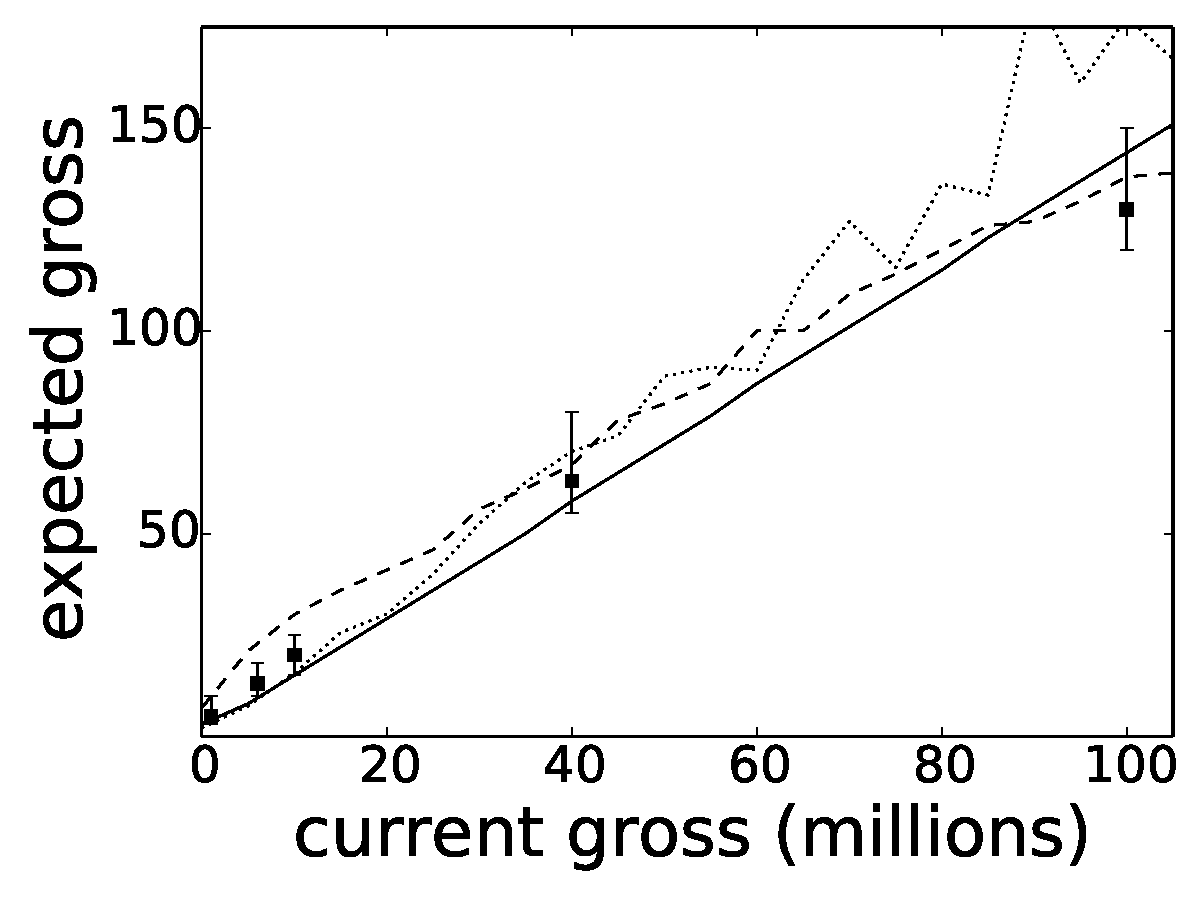
\includegraphics[width=1.0\textwidth]{predictions_figures/movie_grosses_pred.pdf}
	\end{subfigure}
	\begin{subfigure}{.33\textwidth}
		\caption{Poem lengths}
		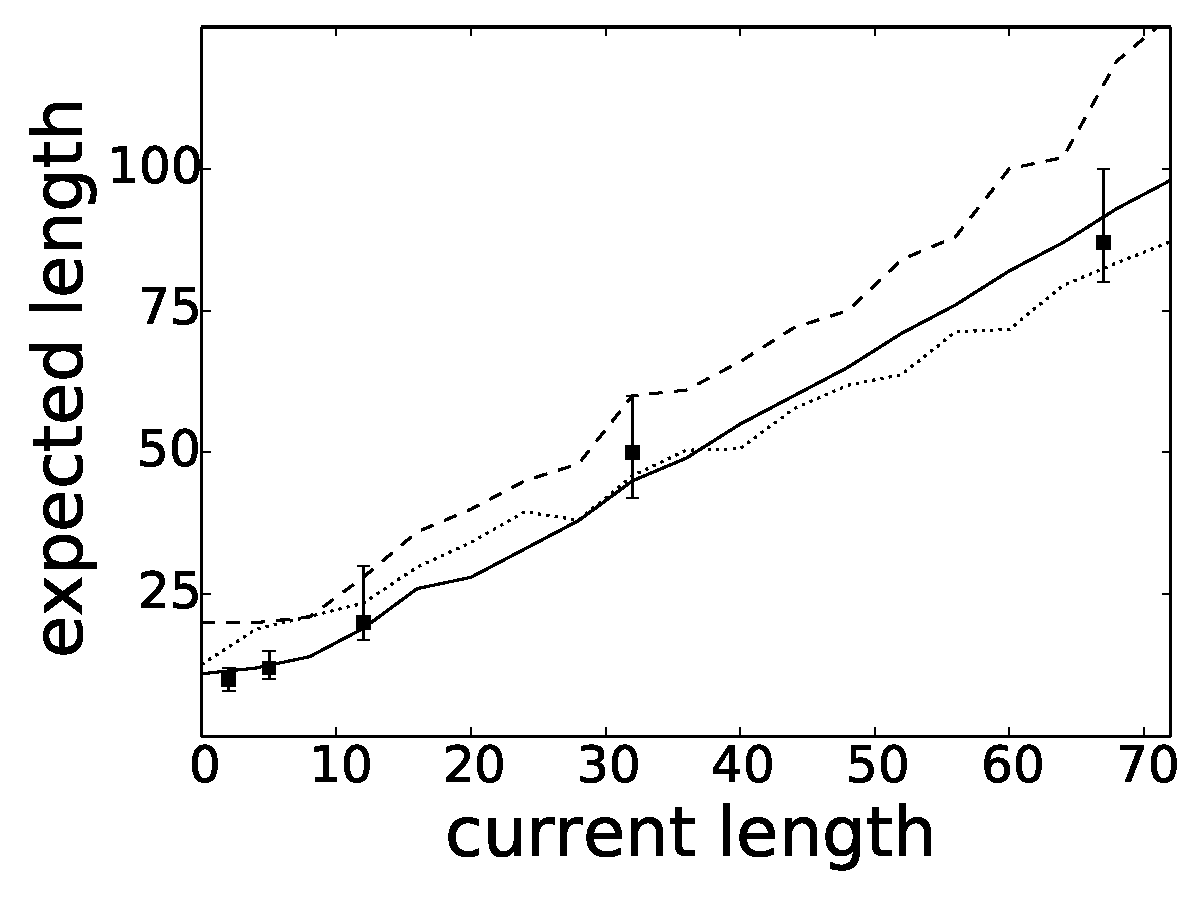
\includegraphics[width=1.0\textwidth]{predictions_figures/poem_lengths_pred.pdf}
	\end{subfigure}
	\begin{subfigure}{.33\textwidth}
		\caption{Lifespans}
		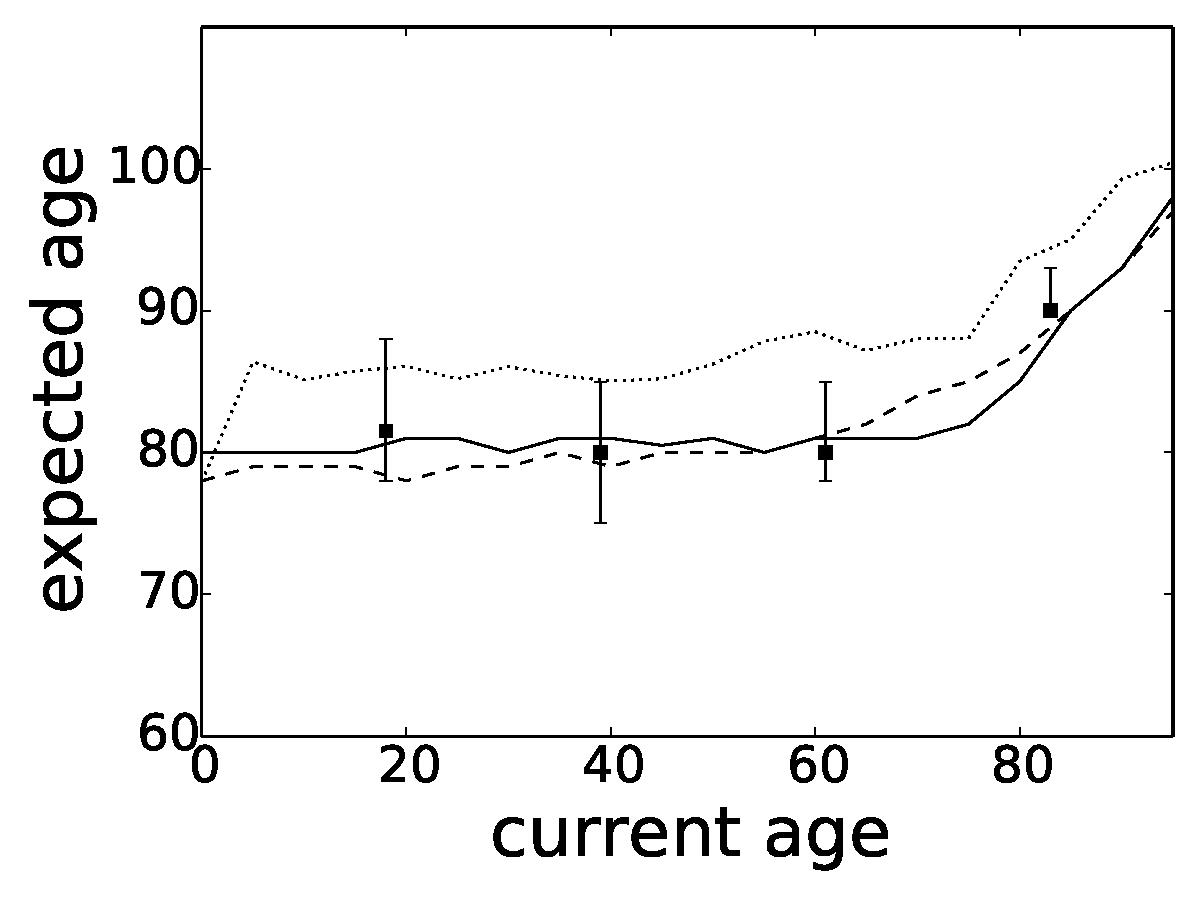
\includegraphics[width=1.0\textwidth]{predictions_figures/life_spans_pred.pdf}
	\end{subfigure}
	}\\
	\makebox[\linewidth][c]{%
	\begin{subfigure}{.33\textwidth}
		\caption{Pharaohs}
		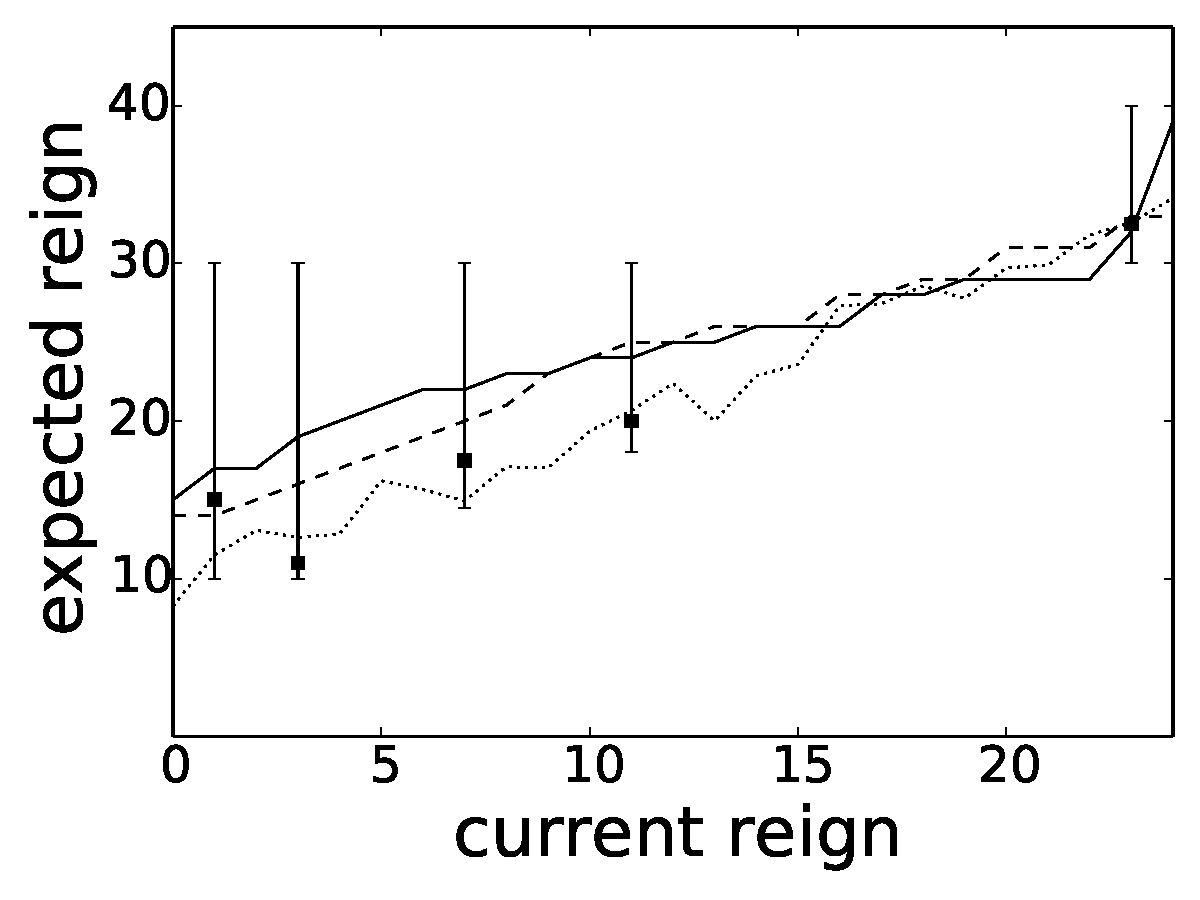
\includegraphics[width=1.0\textwidth]{predictions_figures/pharaohs_reigns_pred.pdf}
	\end{subfigure}
	\begin{subfigure}{.33\textwidth}
		\caption{Movie runtimes}
		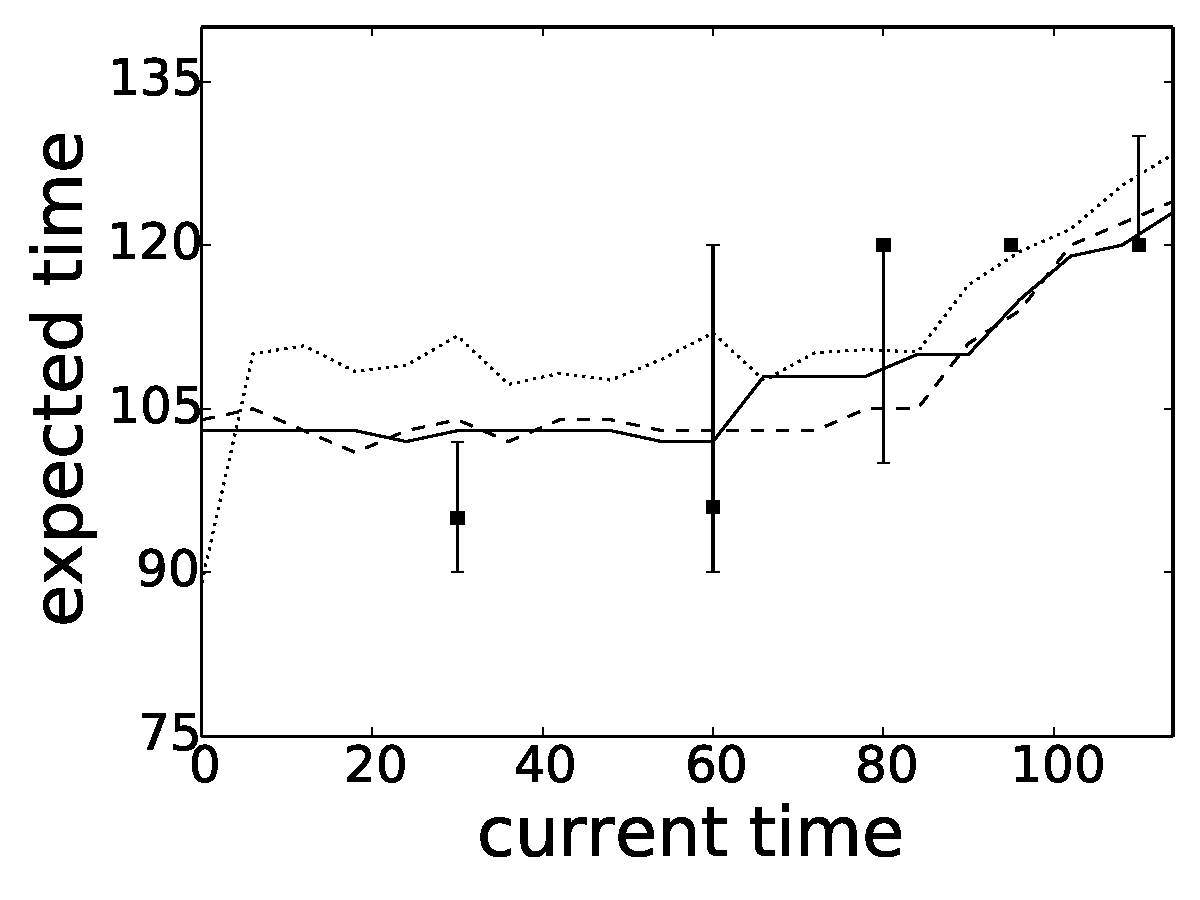
\includegraphics[width=1.0\textwidth]{predictions_figures/movie_runtimes_pred.pdf}
	\end{subfigure}
	\begin{subfigure}{.33\textwidth}
		\caption{Representatives}
		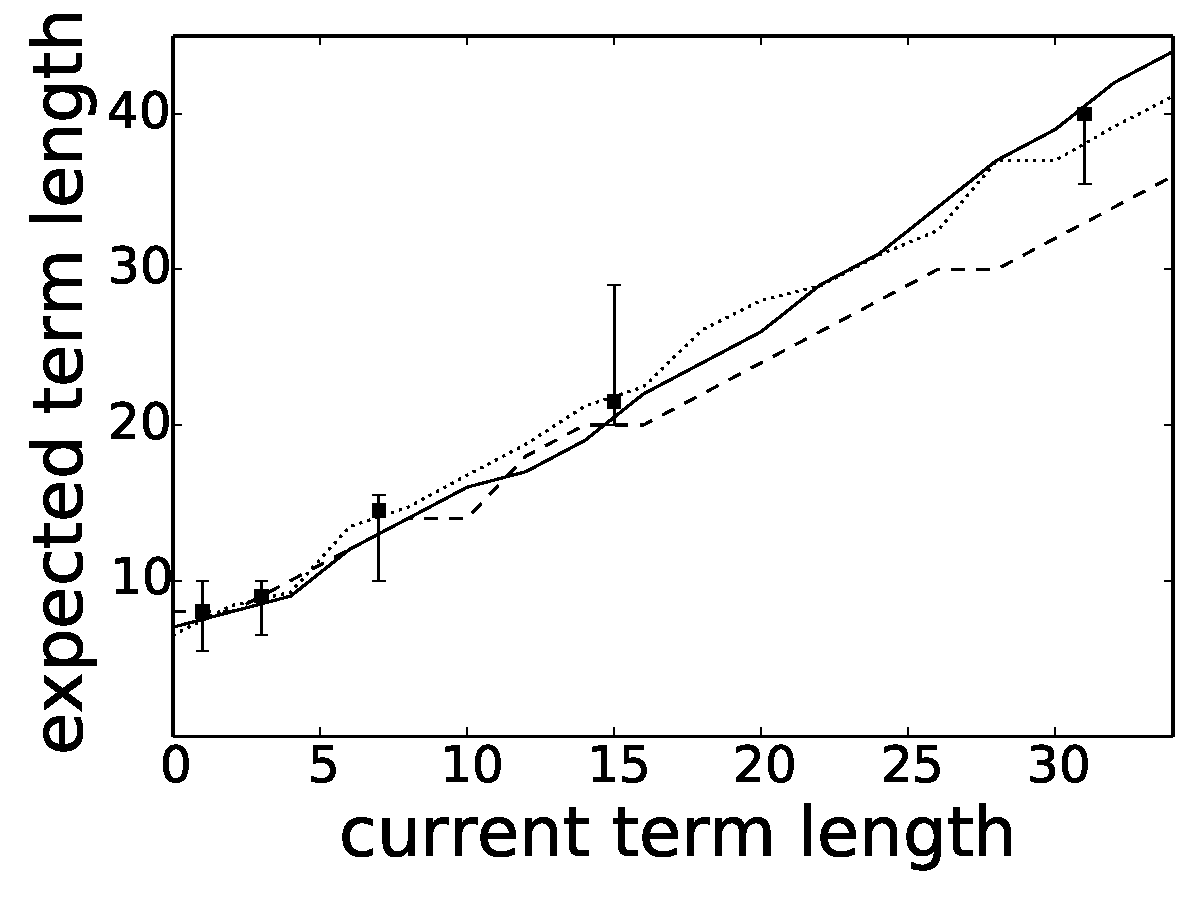
\includegraphics[width=1.0\textwidth]{predictions_figures/representatives_terms_pred.pdf}
	\end{subfigure}
	}\\

	\caption{Replication of the optimal predictions study from GT2. Square markers plot the median empirical response to every question, with error bars plotting bootstrapped $95\%$ confidence intervals. The dashed lines show the posterior median value of $t$ predicted using the optimal predictions model, solid lines show the median posterior predictive responses from the Noisy \mink model, and the dotted lines represent the median posterior predictive responses by the data-driven Bayesian model. All models show good qualitative predictions, with the Noisy \mink fitting the data better than the two Bayesian models.}
	\label{fig:emp_vs_mink_agg_predictive}
\end{figure}


\begin{table}
\centering
\begin{threeparttable}
    \caption{Quantitative measures of model fit to the replication of GT2, using normalized root mean squared error (NRMSE). The Noisy \mink model consistently has the lowest NRMSE scores: assessed solely in terms of the ability to mimic the empirical data it outperforms both of the Bayesian models.}
    \begin{tabular}{llll}
      \toprule
		& \multicolumn{3}{c}{NRMSE}\\
		\midrule
        Question & optimal Bayes & Noisy \mink & descriptive Bayes\\
        \midrule
        Movie grosses & 0.20 & \textbf{0.15} & 0.46\\
		Poem lengths & 0.55 & \textbf{0.10} & 0.19\\
		Lifespans & 0.20 & \textbf{0.10} & 0.66\\
		Pharaohs' reigns & 0.47 & 0.63 & \textbf{0.29}\\
		Movie runtimes & 0.78 & \textbf{0.61} & 0.92\\
		Representatives & 0.24 & 0.10 & \textbf{0.08}\\
      \midrule
    \end{tabular}
    \begin{tablenotes}
      \small
      \item \textit{Note.} The scores with the best results for each question are shown in bold.
    \end{tablenotes}
\label{tbl:nrmse_comparison}
\end{threeparttable}
\end{table}


\bigskip
\subsubsection{Generalizability to new data}

The problem with using descriptive adequacy as the sole measure of model performance is that it is unable to detect overly elaborate models \cite<e.g.,>{myung_importance_2000}. Attempts to correct for model complexity by counting the number of free parameters such as AIC or BIC improve on this a little, but not much. The optimal predictions model produces parameter-free predictions, the Noisy \mink model uses four parameters, and the descriptive Bayesian model uses five. If model evaluations could be safely made by looking only at the number of parameters and the goodness of the data fit, we ought to be able to safely rule out the descriptive Bayesian model: it has more parameters than Noisy \mink and yet produces a worse fit. As it turns out, this intuition is wrong.

To understand why this intuition is incorrect, we consider an alternate method of quantitative comparison known as cross-validation---a standard technique from the model selection literature \cite{browne_cross-validation_2000}---although other options are available such as Bayes factors \cite{wasserman2000bayesian} or approaches specifically geared towards evaluating optimal models using information theory \cite{shen2016}. The central goal in model selection is generally assumed to be to pick the model that will make the best predictions about out-of-sample data, and cross-validation aims to approximate this by estimating parameters on one subset of the empirical data and evaluating performance by measuring how well the model fits capture the held-out data.

To see how all three models generalize to new data, we trained using only a subset of our empirical data, and then tested the models by assessing how well the inferred priors allowed the models to generalize to the withheld data. Specifically, we used $k$-fold cross validation with $k=25$, which involves partitioning the original data set into 25 similarly-sized sub-samples\footnote{For each repetition of the process, between 3 and 5 data points were withheld, with a maximum of one response from a single individual per repetition. The repetitions were balanced so that each data point was withheld exactly once in the entire cross-validation procedure.} and treating each sample once as the unobserved data and the other 24 as the training data. This provides a robust estimate of how each model generalizes to unobserved data.

The results are shown in Table \ref{tbl:cross_validation}. The descriptive Bayesian model has the best overall performance, outperforming the optimal Bayesian model and Noisy \mink in every case. Moreover, although the qualitative comparison in the previous section suggested that Noisy \mink provided a reasonable fit to the data, it performed very poorly in cross validation, far worse than either of the Bayesian models. Despite the apparent simplicity of the Noisy \mink heuristic, it actually corresponds to an overly flexible statistical model for the data. The Noisy \mink model overfits the training data and generalizes poorly to new observations. In contrast, the apparent complexity of the optimal Bayesian model as a psychological theory hides the fact that when viewed as a statistical model for empirical data it is insufficiently flexible, and ends up underfitting the data. The descriptive Bayesian model outperforms them both.


\begin{table}
\centering
\begin{threeparttable}
    \caption{Cross validation model comparisons. In all domains, the data-driven Bayesian model generalizes to new data better than either of the other two models.}
    \begin{tabular}{llll}
      \toprule
		& \multicolumn{3}{c}{Cross validation score}\\
		\midrule
		 & optimal Bayes & descriptive Bayes  & Noisy \mink \\
      \midrule
        Movie grosses & -713 & \textbf{-150} & -100886\\
		Poem lengths & -118 & \textbf{-116} & -3762\\
		Lifespans & -526 & \textbf{-187} & -2327\\
		Pharaohs' reigns & -132 & \textbf{-103} & -2380\\
		Movie runtimes & -258 & \textbf{-153} & -6786\\
		Representatives & -174 & \textbf{-97} & -511\\
		Future lifespans & - & \textbf{-188} & - \\
		Waiting times & - & -91 & - \\
		%\midrule
		\textbf{Average} & -320 & \textbf{-135} & -19442\\
      \midrule
    \end{tabular}
    \begin{tablenotes}
      \small
      \item \textit{Note.} Higher scores (lower absolute values) indicate better generalization. The best score in each row is shown in bold. The bottom row shows the average score for each model across question types. In order to be comparable to the other models, the average score for the data driven Bayesian model is based on the first six rows only.
    \end{tablenotes}
\label{tbl:cross_validation}
\end{threeparttable}
\end{table}

\bigskip
\subsubsection*{Comparing subjective priors to optimal ones}

So far we have seen that, although the descriptive Bayesian framework led us to specify a flexible, statistically complex model, this complexity was justified insofar as this model generalizes to new data better than either the original Bayesian model or the Noisy \mink heuristic. This suggests that there are sound statistical justifications for preferring the descriptive Bayesian model.

However, from a theoretical and psychological perspective, it is not sufficient merely to show that a model is statistically superior to its competitors: A good model should also explain why people behave the way they do. In this respect it is the {\it contrast} between the optimal priors in the GT2 model and the inferred priors extracted by our model that is especially useful. This comparison is shown in Figure \ref{fig:predictions-priors-subjective-vs-empirical}, and is instructive both in terms of the similarities and the differences in reveals. Inspection of this figure suggests that although people's subjective priors are similar to the true environmental distributions, there are systematic deviations in most cases: People's prior expectations about movie run times and representative term lengths both seem to be too long, and their beliefs about lifespan distributions seem to underestimate infant and child mortality rates.\footnote{Note that the latter may be partly due to the limitations of the experimental design and the model, given that the model does not make it easy to estimate negatively skewed distributions and the experiment does not ask questions that tease apart people's beliefs about infant mortality.} The distribution of future lifespans does not have a veridical value, but the descriptive model infers something that seems sensible: It has a similar form to the subjective prior for actual life spans, but is shifted to the right with an average life span of 105. That said, in spite of the minor differences the overall degree of agreement between the two Bayesian models is remarkable, especially given that the built in assumptions about participant priors in the descriptive model were fairly weak.


\begin{figure}[t]
	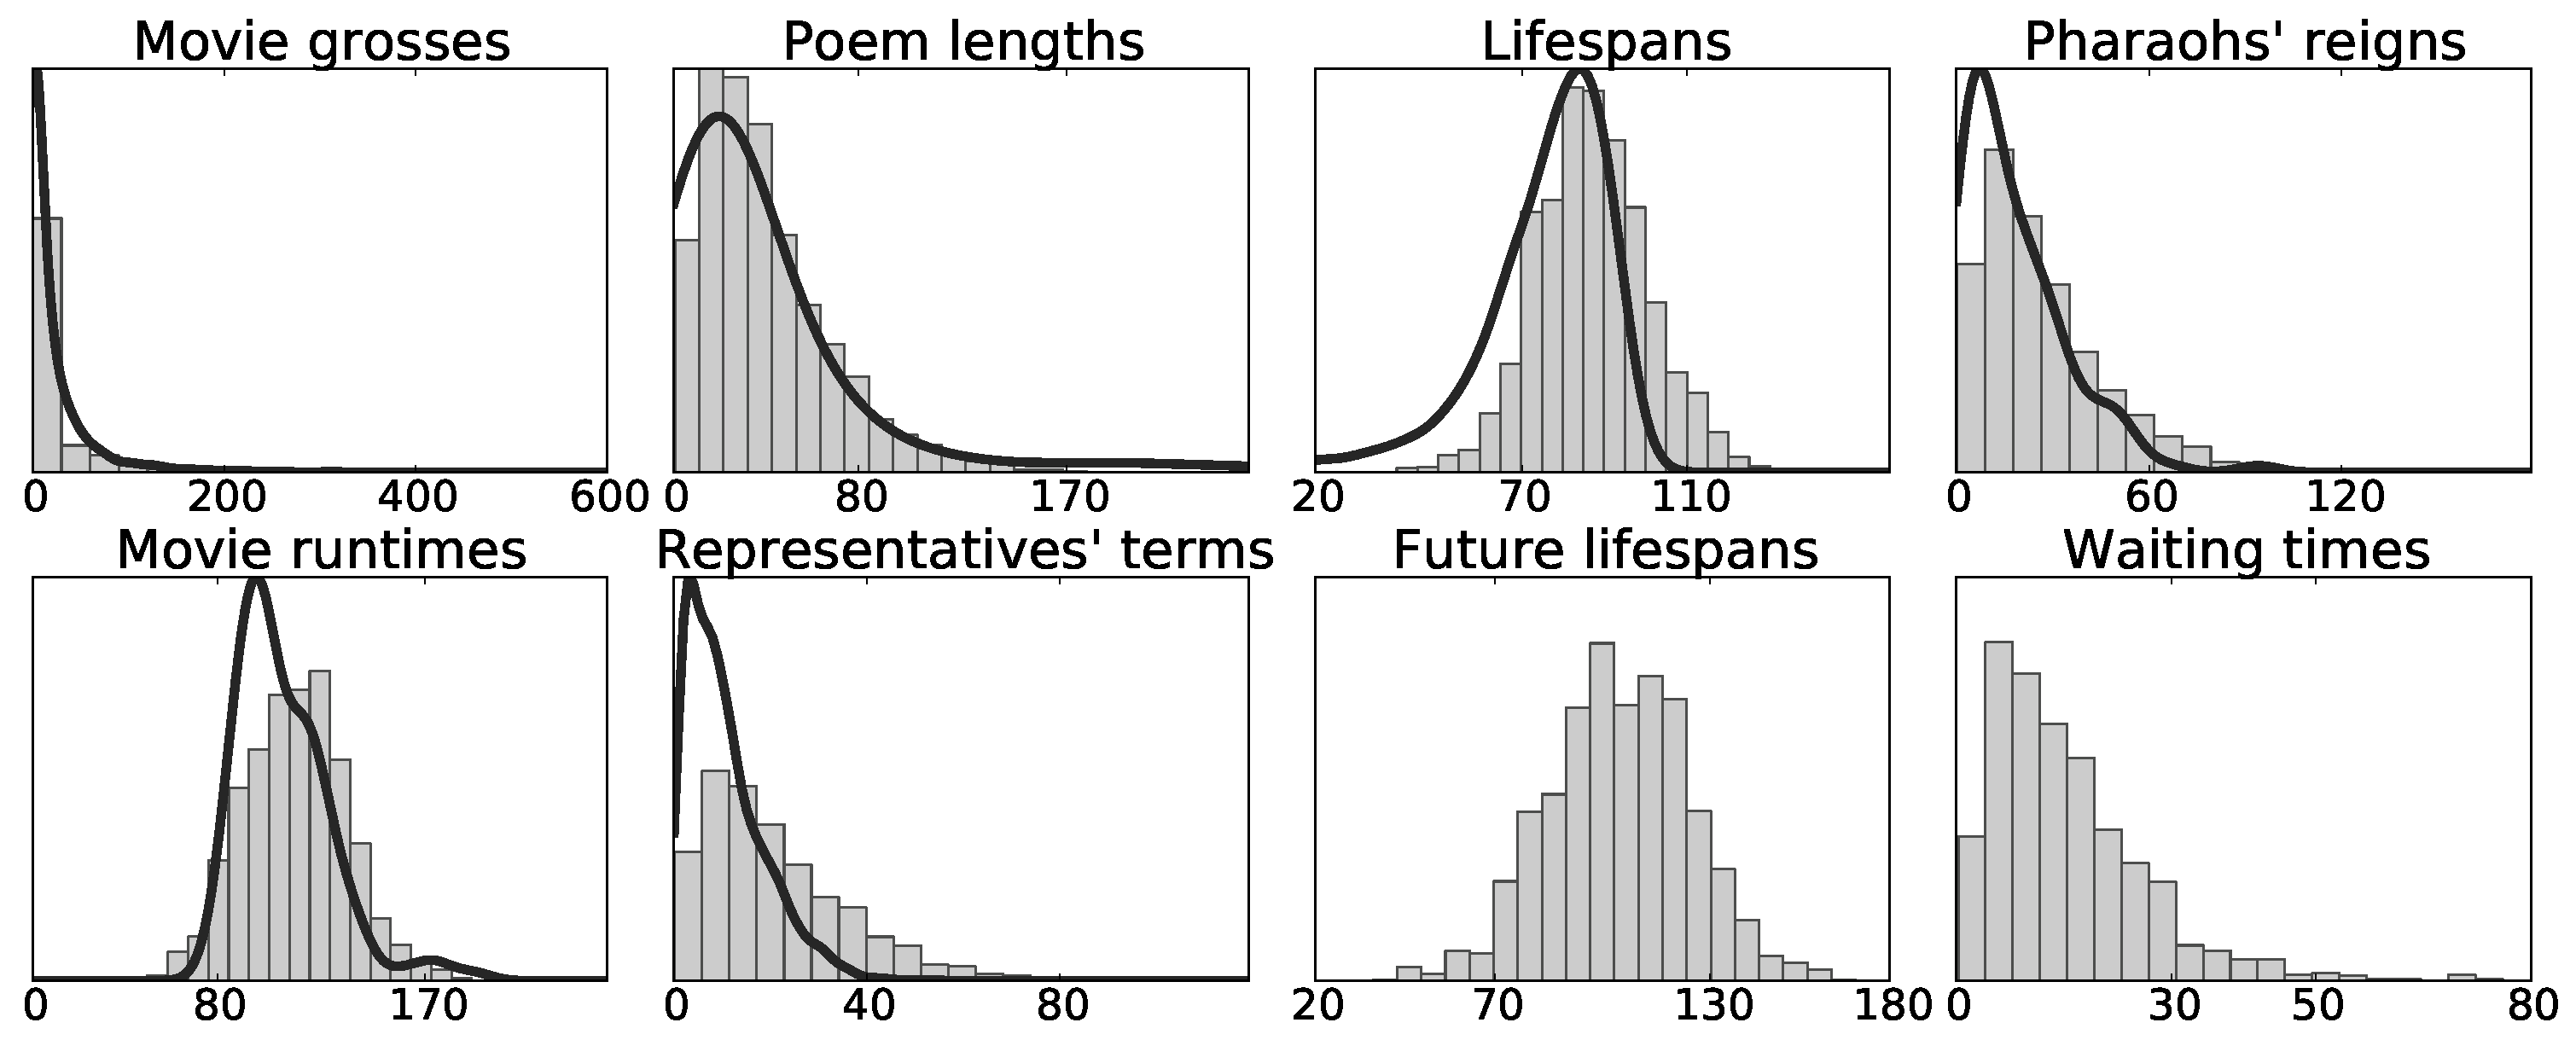
\includegraphics[width=1.0\textwidth]{predictions_figures/priors-subjective-vs-empirical.pdf}
	\caption{Estimates of people's subjective prior beliefs (histograms) compared with the environmental distributions collected by GT2 (lines). In most cases the estimates are similar to the true distributions, although people often underestimate the frequency of events at lower numbers. There was no environmental data available for future lifespans and waiting times.}
	\label{fig:predictions-priors-subjective-vs-empirical}
\end{figure}



\subsection*{Discussion}

Whereas the take-home point from the first case study was that descriptive Bayesian models can be psychologically revealing even when optimal Bayesian models are wrong, the second case study tells a very different story, one in which the exploratory and data-driven analysis based on descriptive Bayesian models complements the original optimal Bayesian model.  Although the optimal predictions model from GT2 is not the best performing model either in terms of the data fit (Noisy \mink is best) or generalizability (descriptive Bayes is best), we found it almost impossible avoid the conclusion that the original rational analysis was remarkably successful.  It is true that the estimated priors plotted in Figure~\ref{fig:predictions-priors-subjective-vs-empirical} do show systematic differences from the optimal ones, which explains why the optimal predictions model does not win in the model selection exercise. These deviations, which we would not have known about without the descriptive Bayesian model, are cognitively interesting; but even so, the similarities between the estimated priors and the veridical ones are much more striking than the differences.

In this instance, the descriptive Bayesian approach reinforces the conclusions from the original rational analysis. Indeed, because of the descriptive Bayesian approach, we feel far {\it more} confident in drawing conclusions about (near-)optimality than we did based on the optimal model only: The descriptive model was afforded the freedom to choose whatever prior distribution (from a very broad family) best accommodated the empirical data, but the end result was a collection priors that are only very slightly different to the veridical ones used by GT2. In our view this provides much stronger evidence for optimality than the original analysis, which showed a qualitative agreement between the optimal model and empiricial data but did not include any formal model comparisons.

When contrasting the descriptive and optimal Bayesian approaches, it is worth noting that {\it any} choices made by researchers are going to incorporate biases of some sort. After all, we have to make {\it some} assumptions about the family of priors people might have, or the type of likelihood functions, and so forth. For example, the assumptions that we built in to the descriptive model were shaped by previous research and our own goals as researchers. We are not arguing that the descriptive approach cannot fall prey to these problems; they are an inevitable part of doing science within any modeling framework.  However, the descriptive Bayesian approach (a) allows us to build in fewer assumptions---e.g. a family of distributions allows for many more possibilities than a single one---and (b) more importantly, does not require that those assumptions be justified on the basis of optimality. GT2 were forced by the straightjacket of optimal Bayesian modeling to have to claim that the distributions they chose were justified on the basis that they were well-matched to the real world. We were forced to make no such claim; we simply chose a family of distributions based on what was sensible and then observed which of those best fit the pattern of human performance.

Of course, some cautionary notes should be attached to these results. For instance, to avoid covering the same ground as the first case study we have not developed a Bayesian model that accounts for individual differences. Similarly, our discussion of the Noisy \mink model in this section has been more cursory than the model deserves purely because our focus is on different kinds of Bayesian models. As an example, our data analysis automatically produces estimates of the multiplier parameter $g$ as well as specific exemplars that the Noisy \mink model uses to generate responses. Other variations on Noisy \mink might perform better, and we do not think strong conclusions about the relative merits of Bayesian and heuristic models should be drawn from these analyses. Even so, the model comparisons here highlight the manner in which it is possible to make sensible comparisons between optimal Bayesian models, non-optimal heuristic models, and descriptive Bayesian models, so long as good statistical procedures are used to guide the comparison.





\section*{Case study 3: A descriptive approach can be relevant even when questions about optimality are not}

The first two case studies differed in several respects and led us to different theoretical conclusions about the optimality of human reasoning in the two problems considered, but one attribute they share is the very fact that optimal models and descriptive models are both applicable to the problem. This is not always the case. In many situations a Bayesian model serves a useful purpose even when no clear notion of ``optimality'' seems to apply. Probabilistic topic models \cite{steyvers_probabilistic_2007}, for instance, are often used as tools for exploring human semantic knowledge, but the scientific utility of these models is not generally taken to justify any claim about human {\it optimality}. In such situations it may be convenient to use a Bayesian model, but the primary intention is to use the model as a tool. Applying a Bayesian model in this fashion aligns naturally with the descriptive Bayesian framework, because the researcher merely claims that the Bayesian model produces similar behavior to humans and does not use a good model fit to justify an optimality claim.

Our third case study presents one such example, using an existing Bayesian model of inductive generalization as a tool to explore the hypotheses that might guide people's intuitions in simple reasoning problems. The goal here is to highlight the fact that very often researchers can use descriptive Bayesian models productively, even in situations where questions about the ``optimality'' of human cognition do not seem especially relevant to the research question.


\subsection{Inductive generalization as Bayesian reasoning}

The Bayesian theory of generalization developed by \citeA{Tenenbaum2001} (henceforth TG1) formalized the problem of inductive generalization in the following way. Suppose a learner is told that some set of entities $X = \lbrace x_1,. . ., x_n \rbrace$ all possess some property $P$, and is asked to infer whether a new entity $y$ also shares that property. Suppose also that the learner is equipped with some {\it hypothesis space} $\mathcal{H}$ that consists of all hypotheses $h$ that the learner considers for the extension of the property $P$, and a prior $P(h)$ over these hypotheses that describes how plausible the learner considers each hypothesis to be before any data are observed. When told that the entities $X$ possess property $P$, the learner updates their beliefs via Bayes' rule:
$$
P(h | X) \propto P(h) \prod_{i} P(x_i | h)
$$
where $P(x_i | h)$ describes the probability that the entity $x_i$ would be observed to have property $P$ if hypothesis $h$ describes the true extension of that property. Given this posterior distribution the probability that the property extends to the novel entity $y$ is computed by summing the posterior probabilities of all hypotheses $h$ that assert that $y$ possesses $P$:
\begin{equation}
\label{eq:generalization}
P(y \mid X) = \sum_{h:y \in h} P(h \mid X).
\end{equation}
The central feature of the Bayesian generalization model developed by TG1 is the choice of likelihood function, which they referred to as {\it strong sampling}, and assumes that the observed entities are sampled {\it from} the set of entities that possess property $P$. In particular, if observations are sampled randomly from this set, then the probability of observing any specific item $x$ given that the true extension of $P$ is described by hypothesis $h$ is given by
\begin{equation}
P(x \mid h) = \begin{cases}
 \dfrac{1}{\vbars{h}} & \text{if $x\in h$},\\
 0& \text{otherwise}.
\end{cases}
\end{equation}
where $\vbars{h}$ is the {\it size} of the hypothesis $h$, and for hypotheses $h$ that consist of only a finite number of entities the size of the hypothesis corresponds to the number of entities that it contains.

When introducing the model, TG1 noted that this strong sampling model is the central feature of the theory. There are other Bayesian induction models that rely on different sampling models \cite{heit_bayesian_1998,VoorspoelsINPRESS,navarro2012} and there are empirical results suggesting that people can change their sampling assumptions to suit the context \cite{RansomINPRESS,VoorspoelsINPRESS,gweon_infants_2010}. Nevertheless, there is considerable evidence that it works well as a default model for inductive generalization \cite{sanjana_bayesian_2003}.

\subsection{The hypothesis space problem}

The biggest practical difficulty that arises when applying the Bayesian generalization model is the fact that---although it provides an unambiguous specification of the likelihood function $P(x|h)$---it places few if any constraints on the choice of hypothesis space $\mathcal{H}$ or the prior distribution $P(h)$ defined over that space. The original work by \citeA{shepard_toward_1987} assumed that hypotheses corresponded to connected regions within a suitably formulated psychological space \cite<and estimated by multidimensional scaling or similar methods:>{torgerson_theory_1958,borg_modern_2005}. However, TG1 proposed that the Bayesian generalization model could be applied more widely than this, including in cases where the stimuli are defined in terms of a set of discrete features \cite<estimated using additive clustering or similar methods: >{shepard_additive_1979,lee_generating_2002,navarro2008}.

This extension of the model is one of the more innovative elements to the TG1 work, but introduces a problem for the researcher. If the goal is to study how people generalize from stimuli, what hypothesis space should we assume they use to guide their inferences and what priors over those hypotheses are sensible? The original TG1 paper notes this issue, but does not propose a solution. In applications of the model researchers have tended to fall back on the traditional solution of trying to infer mental representations (and by extension hypothesis spaces) from a set of similarity judgments. For instance, \citeA{sanjana_bayesian_2003} used a hierarchical clustering method to infer a taxonomic tree for a set of animals, whereas \citeA{RansomINPRESS} used a variation of additive clustering to infer a set of hypotheses that allowed for cross-cutting categories. In both cases, the authors relied heavily on the assumption that a set of similarity judgments produced by different participants in a different experiment can be relied upon to constrain the Bayesian generalization model.

An alternative approach to the problem is to estimate a hypothesis space $\mathcal{H}$ from the generalization judgments themselves. Multidimensional scaling and additive clustering are statistical techniques that rely upon psychological theories of similarity judgment (e.g., geometric similarity models, feature contrast models) to provide the link between empirical data and the inferred mental representation. However, if the goal is to learn something about the hypotheses that constrain people's generalizations, it seems to make more sense to use a psychological theory of generalization to do to the work.


\subsection*{Experiment}

The data for this case study come from a property induction task \cite<e.g.,>{osherson_category-based_1990}. In it, participants are presented with one or more examples that share a novel property and are then asked to rate the probability that additional exemplars also possess that property. Data were collected from 762 workers on Amazon Mechanical Turk who were paid \$0.50 for completing the $10$-minute study. After a pretest designed to ensure that people understood the task, they were given the following question:

\begin{quote}
{\it In the past, scientists discovered that all $\mathbf{A}$ have an enzyme called Enzyme-Q. What is the probability that each of the following animals also have Enzyme-Q?}
\end{quote}

\noindent
The known exemplar $\mathbf{A}$ was one of the following 20 mammals: \stimulus{bats, beavers, chimps, cows, dolphins, elephants, gorillas, horses, kangaroos, koalas, mice, pandas, polar bears, rabbits, rhinos, seals, squirrels, tigers, whales}, or \stimulus{wolves}. People were asked to give probability judgments for all 20 the mammals by moving a slider between 0\% and 100\%. After providing probability judgments for all of the mammals, all of the sliders were reset to 0\% and people were given the following additional information:
\begin{quote}
{\it Later, scientists discovered that in addition to $\mathbf{A}$, all $\mathbf{B}$ also have Enzyme-Q. Given this new information, what is the probability that each animal has Enzyme-Q?}
\end{quote}

\noindent
The first exemplar \textbf{A} remained unchanged, and the second exemplar \textbf{B} was one of the remaining mammals other than \textbf{A}. Trials were balanced so that each of the 190 possible combinations of two mammals occurred approximately four times across all participants.


\subsection*{Results}

We excluded from analysis 175 participants who either failed to follow the instructions on the pretest, or did not rate mammals as having a property with 100\% certainty when they were told the mammal had that property in the instructions. Results are based on analysis of the remaining 587 participants.

\begin{figure}[p]
\begin{center}
\begin{tabular}{cc}
	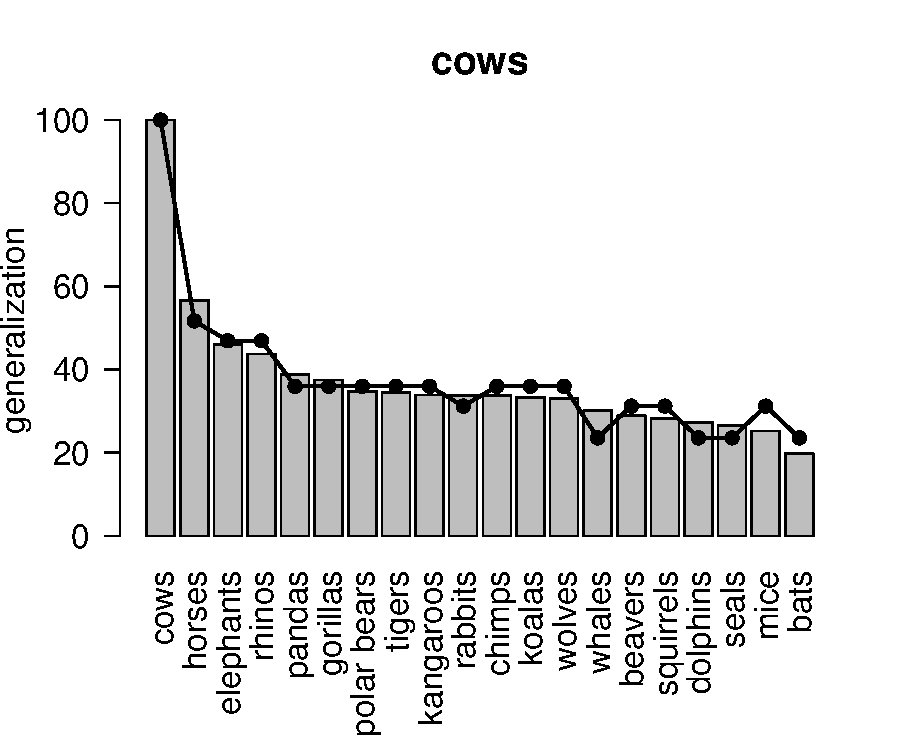
\includegraphics[width=6.5cm]{generalization_figs/cows.pdf} &
	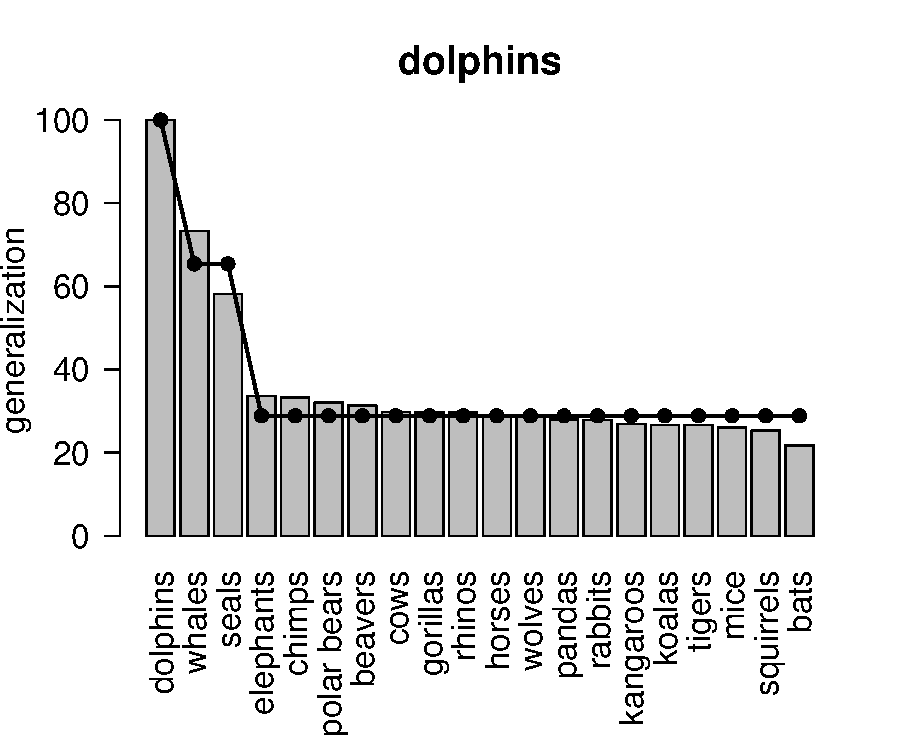
\includegraphics[width=6.5cm]{generalization_figs/dolphins.pdf} \\
	(a) & (d) \\
	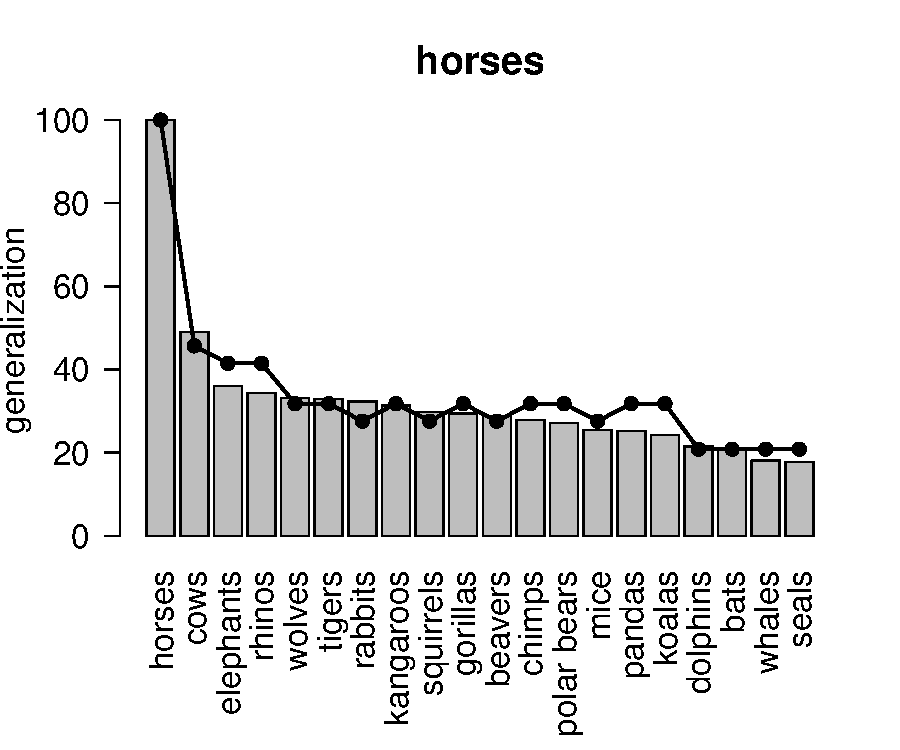
\includegraphics[width=6.5cm]{generalization_figs/horses.pdf} &
	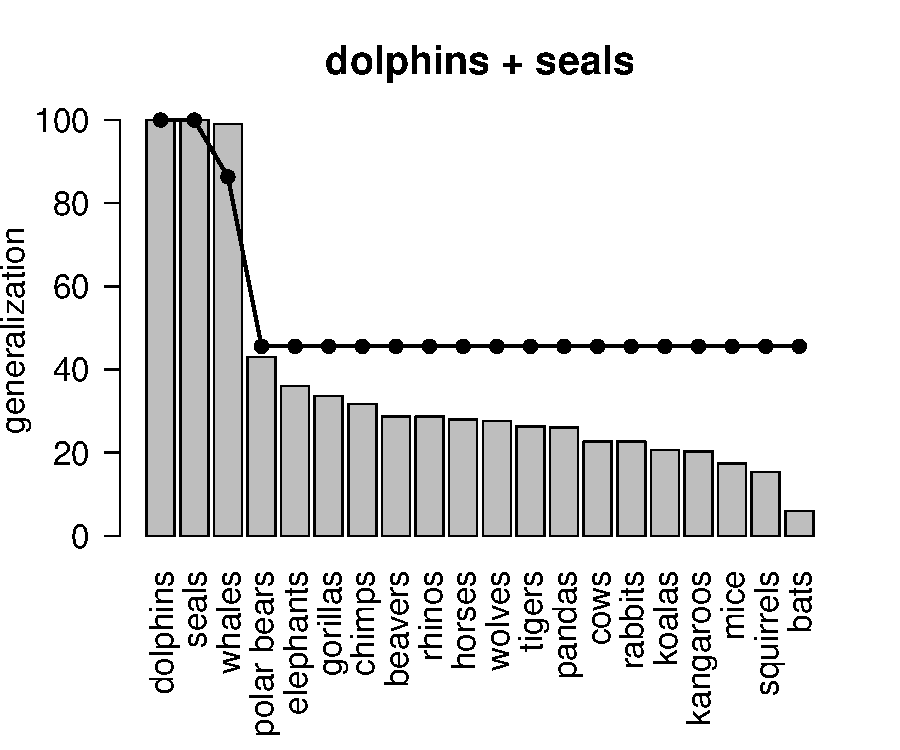
\includegraphics[width=6.5cm]{generalization_figs/dolphinsseals.pdf} \\
	(b) & (e) \\
	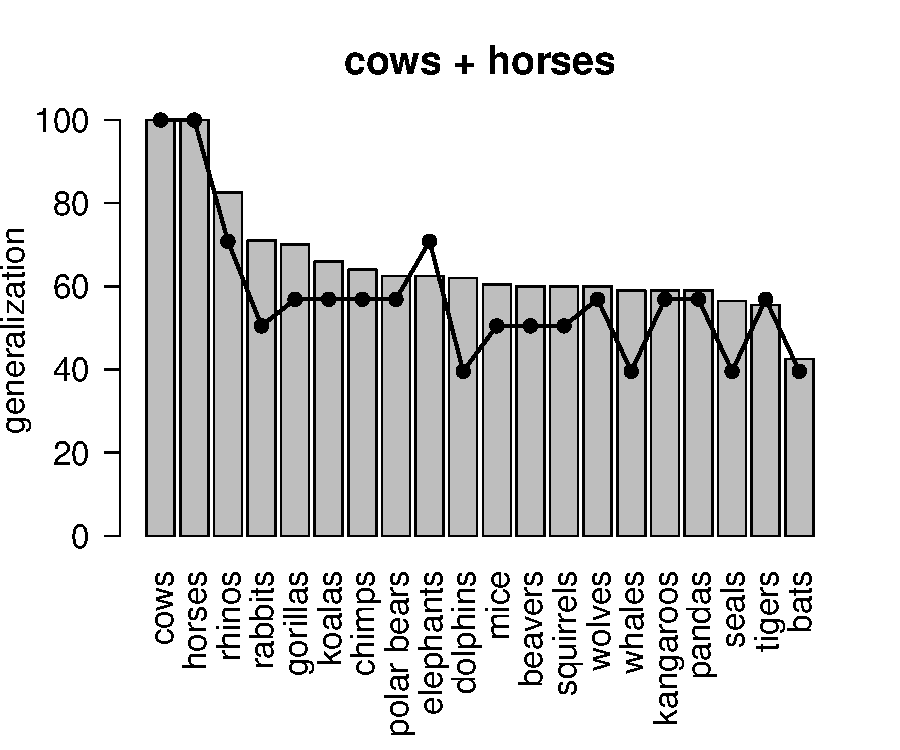
\includegraphics[width=6.5cm]{generalization_figs/cowshorses.pdf} &
	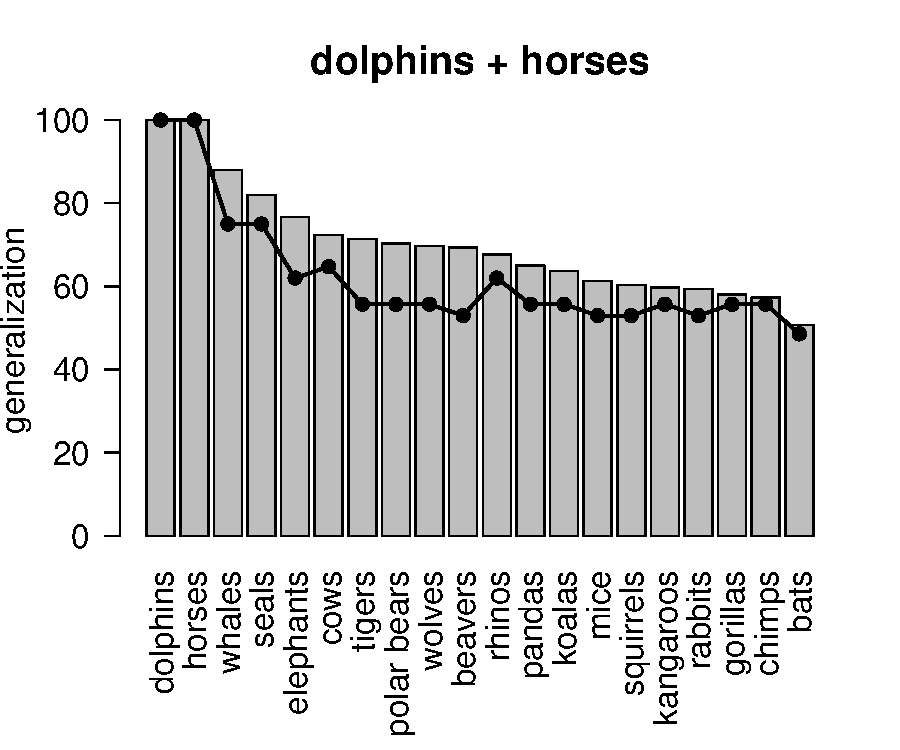
\includegraphics[width=6.5cm]{generalization_figs/dolphinshorses.pdf} \\
	(c) & (f) \\
\end{tabular}
\vspace*{12pt}
\caption{Example generalization gradients produced by human participants (bars) compared to those estimated with the help of the Bayesian generalization model (solid lines). In each case, the title of the plot indicates which item(s) were known to possess Enzyme-Q, and the generalization targets are arranged in order of decreasing (human) generalization probability.}
\label{fig:gen_posterior_pred}
\end{center}
\end{figure}

\bigskip
\subsubsection*{Human generalization data}

Representative generalization patterns from human participants are shown in Figure~\ref{fig:gen_posterior_pred}, and seem very sensible. When told that {\it cows} have Enzyme-Q people are most willing to extend that property to \stimulus{horses} (panel a) and vice versa (panel b). When told that Enzyme-Q is possessed by both \stimulus{cows} and \stimulus{horses}, people tended to extend the property far more widely (panel c): In this instance, our participants showed the {\it premise monotonicity} effect in which adding more positive examples causes people to generalize more widely. However, in other instances people showed the opposite {\it premise non-monotonicity} effect. For instance, compare the generalization gradients from \stimulus{dolphins} (panel d) to those from both \stimulus{dolphins} and \stimulus{seals} (panel e). The addition of the second exemplar increases the probability of some items (e.g., \stimulus{whales} shows premise monotonicity in this case) but decreases the probability of others (e.g., \stimulus{bats} shows non-monotonicity).

This pattern, in which some generalizations show monotonicity effects and others non-monotonicity is generally explained by noting that some pairs of premise items tend to ``call attention'' to a specific category. Adding \stimulus{seals} to \stimulus{dolphins} strongly suggests that the true extension of the property is {\it marine mammals} and so the probability that \stimulus{whales} possess the property increases, and the probability hat \stimulus{bats} do so decreases. Moreover, when ``given'' the right set of categories upon which to base its inductive inferences, Bayesian generalization models capture this pattern perfectly well \cite<e.g.,>{RansomINPRESS}. However, this raises the question: How do we know {\it which} categories people people perceive to be relevant to the inductive generalization problem? It seems obvious that when reasoning about \stimulus{dolphins} and \stimulus{whales}, the category of {\it marine mammals} is relevant. This would explain the pattern of generalizations in panels (d)-(f) of Figure~\ref{fig:gen_posterior_pred}. Yet one might also have made the case that {\it farm animals} or {\it ungulants} might be perceived as especially relevant when reasoning about \stimulus{cows} or \stimulus{horses}, but when we compare panel (c) to panels (a) and (b) there is very little evidence for any non-monotonic inferences.

\bigskip
\subsubsection*{Inferring a hypothesis space}

Given the above, how does the researcher work out which categories contributed to the learner's hypothesis space? This seems to be a natural context to apply probabilistic models: The Bayesian generalization model from TG1 supplies a theory that says, given {\it this} hypothesis space $\mathcal{H}$ and {\it that} prior $P(h)$ defined over it, then people should be expected to make {\it these} generalizations. We can use statistical methods to invert this: If we assume people produced those generalizations using this psychological model, what hypothesis space is required to support it? However, although the Bayesian framework is ideally suited to exactly this kind of work \cite<e.g.,>{navarro2008,kemp_discovery_2008}, it is not at all clear how any notion of {\it optimality} is relevant to this sort of problem. If we use the generalization model to infer a hypothesis space $\mathcal{H}$, does that mean that it is ``rational'' to use $\mathcal{H}$? Are we committed to a claim that people were reasoning rationally given those hypotheses? We are not at all convinced that either of these are true. Nevertheless, the underlying {\it descriptive} goal is an intriguing one: Can we use the TG1 model as a {\it tool} to learn something about the mental representations and hypotheses that people use to guide their generalizations? Bayesian optimality is quite irrelevant to this goal, but Bayesian description is very relevant indeed.

Our approach is loosely based on the additive clustering model for extracting discrete categories from similarity judgments \cite{shepard_additive_1979} and adapted to the inductive generalization context using the model from TG1. We assume that the ``base'' hypothesis space $\mathcal{H}$ consists of a set of categories that can be described by the binary matrix $\mathbf{C}$ such that $c_{ik}=1$ if the $i$-th item belongs to the $k$-th category, and $c_{ik}=0$ if it does not. Some of the categories are fixed {\it a priori}: We assume that there exists a ``singleton'' category for each animal (e.g., one possibility is that the property holds for \stimulus{dolphins} only), and we assume that there exists a ``universal'' category (i.e., the property is true for all mammals). We impose no other {\it a priori} constraints on the structure of the category matrix $\mathbf{C}$.

In order to construct the generalization probabilities for the Bayesian model, we follow \citeA{navarro2012} in allowing the model to {\it learn} the extent to which people use strong sampling or weak sampling, indexed using a single parameter $\theta$ (where $\theta=0$ implies weak sampling, and $\theta = 1$ implies strong sampling). Similarly, we follow \citeA{sanjana_bayesian_2003} in allowing {\it composite} hypothesis spaces in which the property in question might be possessed by two of the categories in $\mathbf{C}$.\footnote{There is nothing special about the number two. There is no reason why the hypothesis space could not include a hypothesis that property $P$ is characteristic of three or more categories. However, given that we never presented people with more than two premise items, the limitation to two seems sensible.} The model includes a free parameter $\gamma$ corresponding to the relative weight given to simple hypotheses where the property is assumed to be a characteristic of a single category, versus composite ones in which it is assumed to be a property of multiple categories. When $\gamma = 0$ all generalizations from multiple items rely on simple hypotheses only, whereas setting $\gamma = 1$ produces generalizations from composite hypotheses. The model is described in detail in Appendix C, along with details of how we estimate the category assignment matrix $\mathbf{C}$, the prior weights assigned to the categories, and the free parameters $\theta$ and $\gamma$.

\bigskip
\subsubsection*{Applying the model}

\begin{table}[t]
\caption{The categories inferred using the Bayesian generalization model. Additionally, the model included singleton categories (e.g., ``just dolphins'') and the universal category (i.e., ``all mammals''). \vspace*{6pt}}
\begin{center}
\begin{tabular}{p{7cm} | l | p{3cm}}
\textbf{hypothesis}	&	\textbf{prior} &	\textbf{interpretation}	\\
\hline
tigers, wolves & 0.089 & big predators \vspace*{3pt}\\
chimps, gorillas & 0.036 & primates \\
dolphins, seals, whales & 0.032 & marine mammals \\
bats, beavers, mice, rabbits, squirrels & 0.022 & rodents \\
koalas, pandas, polar bears & 0.022 & ``bears'' \\
cows, elephants, horses, rhinos & 0.019 & hoofed animals \vspace*{3pt}\\
beavers, chimps, cows, elephants, gorillas, horses, kangaroos, koalas, mice, pandas, polar bears, rabbits, rhinos, squirrels, tigers, wolves\vspace*{3pt} & 0.012 & non-marine, non-flying mammals  \\
chimps, cows, gorillas, horses, kangaroos, koalas, pandas, polar bears, tigers, wolves & 0.007 & medium-sized land mammals \\
\hline
\end{tabular}
\end{center}
\label{table:hypothesis_space}
\end{table}


The hypothesis space and priors that we estimated consists of the 9 categories listed in Table~\ref{table:hypothesis_space} and visualized in Figure~\ref{fig:hypothesis_space} (singleton categories and the universal category are omitted). The categories are generally sensible ones, and the generalization gradients that they produce are a reasonable approximation to human generalizations (e.g., solid lines in Figure~\ref{fig:gen_posterior_pred}). Some of the categories have a taxonomic basis (e.g., {\it primates}), others are superficial resemblances (e.g., \stimulus{koala} are unrelated to \stimulus{pandas}), and others are based on ecological roles (e.g., {\it large predator}). As a consequence, the overall structure of the categories people used to guide inductive inferences is non-hierarchical and cross-cutting.

The parameter estimates are also revealing. The best fitting model parameters were $\theta=0.09$, which suggests that people tended not to rely on a strong sampling assumption. This pattern is consistent with earlier results \cite{navarro2012,RansomINPRESS}, and indeed has some resemblances with the ``conservative'' inferences in our first case study. The best fitting parameter value of $\gamma=0.91$ indicates that people had a strong tendency to rely on composite hypotheses when generalizing from multiple exemplars. This pattern is consistent with the approach taken by \citeA{sanjana_bayesian_2003}. Finally, when evaluating the overall performance of the Bayesian model, it is interesting to compare the model against human responses separately for those trials in which people were asked to generalize from a single exemplar versus when they were asked to generalize from multiple exemplars. As Figure~\ref{fig:gen_fit} illustrates, the model does a very good job of producing human like generalizations from a single exemplar (panel a; $r=0.93$), but the fits are rather less impressive for the trials when generalizations from two exemplars are requested (panel b; $r=0.76$), suggesting that there is still something missing from the Bayesian generalization framework.

\begin{figure}[p]
\begin{center}
\bigskip
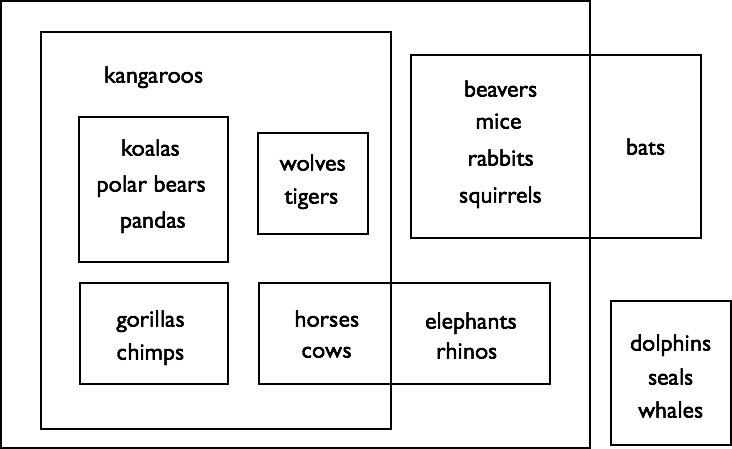
\includegraphics[width=.6\textwidth]{generalization_figs/hypotheses.png}
\bigskip
\caption{Visualization of the categories estimated from human inductive generalizations with the assistance of a Bayesian model. As is clear from inspection, the category structure is non-hierarchical and includes a number of cross-cutting categories.}
\label{fig:hypothesis_space}
\end{center}
\end{figure}

\begin{figure}[p]
\begin{center}
	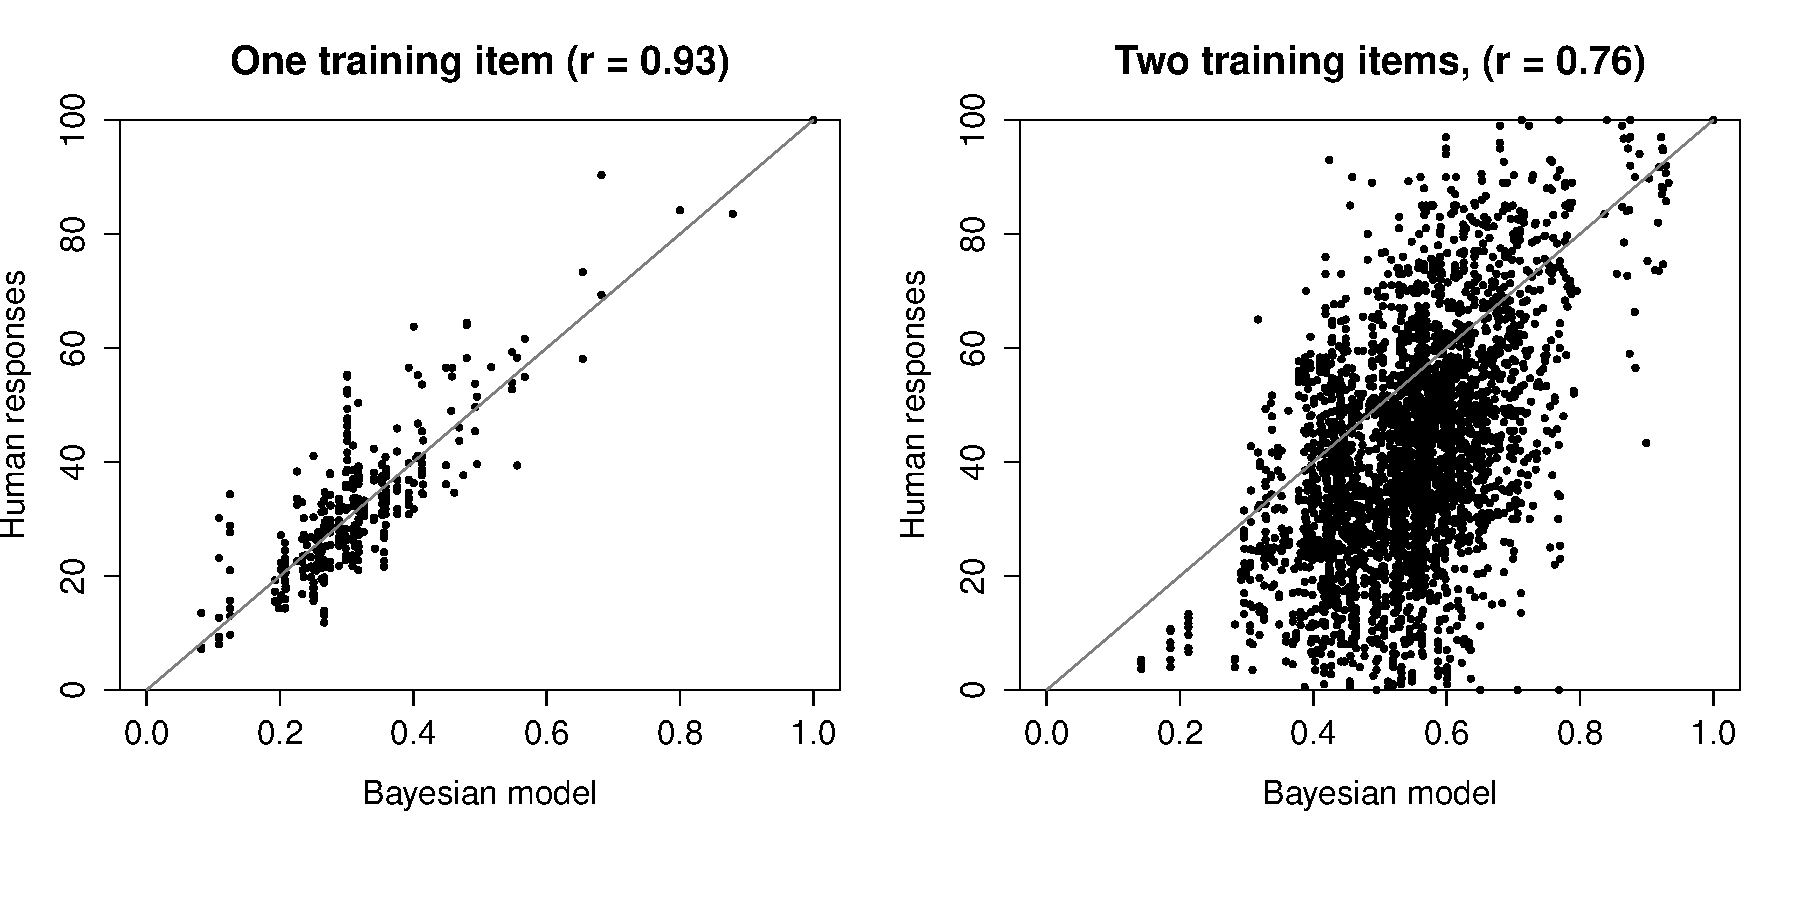
\includegraphics[width=14cm]{generalization_figs/allitems.pdf}
\vspace*{12pt}
\caption{Comparing the model predictions against human responses. The left panel plots all 380 pairs of stimuli for which we obtained generalization judgments, and the right panel plots all 3760 triads for which we did so. The inferred hypothesis space produces generalization probabilities that provide a very good account of those trials in which participants were asked to generalize from a single exemplar (the correlation on the left panel is $r=0.93$), and are adequate ($r=0.76$) when predicting generalizations from multiple items.}
\label{fig:gen_fit}
\end{center}
\end{figure}

\subsection*{Discussion}

The central point in our third case study is that using a Bayesian model as a general purpose, descriptive model can be extremely useful as a tool for exploring mental representations. Our application in this instance is a relatively simple example, and is a natural way of extending the framework developed by TG1, but it addresses a fundamental problem in cognitive science, by exploring the hypothesis spaces that underpin human inductive inferences. In light of our results, the utility of Bayesian cognitive models seem obvious. By supplying a probabilistic model for human behavior that links a hypothesis space to an observable response, we can reverse engineer the process and seek to infer the hypothesis space itself. Although we admit to a degree of bias ourselves, it is hard not be interested in results suggesting that people in this task relied more heavily on composite hypotheses and used a weak sampling model. Having found that the Bayesian model works better at capturing generalizations from a single exemplar than from two exemplars, we are motivated to ask why this might be so. We do not know the answer ourselves, but this analysis opened up many useful questions for further exploration.

This case study highlights another point worth making. The descriptive Bayesian approach might provide a partial solution to a common problem within cognitive modeling: the fact that in some situations internal representations, like the hypotheses used by the learner, might not always be recoverable. This occurs when the parameters of the model (which for Bayesian models includes choices of prior and likelihood) are underconstrained by the data \cite<see, e.g.,>{mamassianlandy2010}. The descriptive approach, which performs inference over possible priors and likelihoods, may help by providing researchers with some guidance about whether these choices are reliably constrained by the data.

More importantly for the purposes of the current paper, the importance of these findings seems to be largely unconnected to {\it any} notion of human ``optimality.'' Our analysis used the TG1 model in an entirely pragmatic fashion, as a tool to help us explore people's hypothesis spaces and open up new questions about the inductive biases that guide inductive reasoning. Similarly, it does not seem entirely on point to be asking whether it would be rational for our participants to rely on the categories listed in Table~\ref{table:hypothesis_space}, and thereby make the generalizations they did. To the extent that we have any intuitions about this ourselves, we might be tempted to suggest that people were {\it not} making good judgments: If people really were using a {\it bears} category that lumps \stimulus{koalas} with \stimulus{polar bears} and \stimulus{pandas} as the inductive basis for making generalizations about a biological property (Enzyme-Q), one would hope there is some deeper reason for it other than superficial resemblances.

However, this is very much besides the point: Our goal with this scenario is to illustrate that the model serves a scientifically useful purpose when used in a purely instrumental fashion. In this application at least, the model does not act as a vehicle for us to justify any claim about the rationality or irrationality of human cognition. It is just a useful tool that allows us to learn about the mind. Indeed, we suggest that Bayesian models are often, in practice, used in exactly this fashion: Probabilistic topic models \cite{steyvers_probabilistic_2007}, structure learning models \cite{kemp_discovery_2008} and models for cross-classification \cite{shafto_probabilistic_2011}, for instance, are all Bayesian frameworks for exploring mental representations that do not seem especially reliant on any notion of ``optimality'' to advance their psychological claims. The general philosophy of their approach fits better with the descriptive framework than the Procrustean ``optimal'' framework within which they had to be forced because optimal Bayesian models were the only game in town.

\section*{General Discussion}

\begin{quote}
{\it ``When I use a word,'' Humpty Dumpty said in rather a scornful tone, ``it means just what I choose it to mean---neither more nor less.''} \\
\hspace*{2cm} --- Lewis Carroll, {\it Through the Looking Glass}
\end{quote}

In the final passages of a recent article, \citeA{bowers_is_2012} argued that ``there is a good deal of confusion about what theoretical claims are being advanced by Bayesian modelers'' (p. 426). Although we are frequent advocates of the Bayesian framework ourselves, we find it difficult to disagree with this aspect to their critique. As they note, Bayesian researchers sometimes slide back and forth between making claims about rationality and claims about descriptive adequacy. We have argued that much of this confusion is due to the fact that there are two distinct kinds of model that are subsumed under the term ``Bayesian.'' Optimal Bayesian models can provide a normative standard for human behavior; within that framework, researchers are obligated to provide explicit justifications for their choices of prior and likelihood, showing that the model solves an {\it appropriate} problem. Descriptive Bayesian models impose different obligations on the researcher. Because the researcher has the freedom to specify whatever priors and likelihoods they feel best instantiate their psychological theory, the behavior resulting from the model does not warrant the label ``optimal'' (at least not in any more than the weak sense implied by Dutch book arguments) and the scientific merits of the model must be established on different grounds.


Although our case studies have tended to focus on the value of building descriptive Bayesian models,\footnote{This was motivated in part by a desire to highlight the value of Bayesian models even when no strong claim to optimality is possible.} we do not argue that either approach is {\it inherently} better. They simply represent different kinds of theoretical claims and serve different goals. Each of our three case studies brings this out in a slightly different way:
\begin{itemize}
\item In case study 1, we found that human judgements deviated quite sharply from the predictions of an optimal Bayesian model, but were able to use a descriptive Bayesian model to shed light on how people solved an inductive problem.
\item In case study 2, an analysis based on a descriptive Bayesian model produce nearly identical conclusions to one that relied on an optimal Bayesian model. Although we found minor departures from optimality, the main message that came through is that human cognition in this task was remarkably well-calibrated.
\item Contrasting with both of the previous examples, case study 3 explored a situation in which Bayesian cognitive models can serve a useful scientific purpose even when claims about optimality do not seem pertinent, or at least not relevant to the research question at hand.
\end{itemize}
These three examples are certainly not exhaustive, but we hope that they make clear that the scientific utility of a Bayesian analysis need not be tied to any claim about the optimality of human cognition, and that the success of a Bayesian model does not always imply that human behaviour is especially rational in a particular task.

Much of what we have argued in this paper closely agrees with earlier work. We are hardly the first people to suggest that it is unhelpful to equate ``Bayesian'' with ``optimal'' \cite<e.g. see,>{mckenzie_rational_2003}, and what we have called the ``descriptive view'' has a good deal in common with recent defenses of the Bayesian paradigm \cite{griffiths_how_2012,goodman_relevant_2015}.
Applications of Bayesian models resembling the descriptive approach have increasingly appeared in the literature on cognition \cite<e.g.,>{Hemmer2014, navarro2012, Huszar2010} and perception \cite<e.g.,>{houlsby2013cognitive, zhang2013illusory, acerbi2012internal, battaglia2011haptic, girshick2011cardinal, stocker2006noise, kording2004loss, acerbietal14} with varying levels of clarity about whether or not the models were meant to be explicitly non-optimal or in what degree.
Indeed, it does not seem unreasonable to us to suggest that most Bayesian models are not intended to imply strong claims about optimality of human cognition.

Nevertheless, our view---as Bayesians ourselves---is that if researchers in the field are unsure as to whether and when Bayesian models are intended to justify claims about optimality or rationality (and clearly many people are), then something has gone awry in the way Bayesian models are promoted or designed. In our view considerable confusion results when descriptive claims and optimality claims are conflated. If Bayesians are to avoid contributing to this confusion we should avoid making optimality claims when none are intended, and make sure that we make them only when they are justified.\footnote{We would concede that we have ourselves been guilty of eliding this distinction in some of our own work and, if anything, this serves to strengthen our argument in the current paper. If it is so easy for researchers to accidentally slip into using ``rational analysis'' language when only a descriptive claim is intended, then the need to have distinct nomenclature and a distinct modeling framework is even stronger than it might otherwise appear.} It is our goal with this paper to try to avoid much of this confusion in the future---not only because of the useful rhetorical distinction between {\it descriptive} and {\it optimal}, but also because that rhetorical distinction corresponds to an actual modeling distinction (i.e., whether priors and likelihoods are inferred or stipulated by the scientist). This will, we hope, lead to far less uncertainly about what conclusions one is justified in drawing from the model.


\subsection*{How many different kinds of Bayesian explanation are there?}

\begin{quote}
{\it ``The question is,'' said Alice, ``whether you can make words mean so many different things.''} \\
\hspace*{2cm} --- Lewis Carroll, {\it Through the Looking Glass}
\end{quote}

Throughout the paper we have maintained a strong binary distinction: Some Bayesian analyses make optimality claims; others make purely descriptive claims. This clean distinction is, of course, fiction. In reality every Bayesian model makes a slightly different claim, and it is an oversimplificiation to reduce all this variation to a simple ``optimal versus desciptive'' distinction. Notwithstanding our suggestion that even a crude binary distinction would go a long way towards reducing the ambiguity in the literature, we recognize that nuance is required in practice. For example, in this paper we have described both the GT1 coincidences model (case study 1) and the GT2 optimal predictions model (case study 2) as optimal models, and we would certainly argue that stronger normative claims are licensed by both of those models than either of the descriptive models that we built. The GT1 and GT2 models both use likelihood functions that are justified with reference to a statistical model for the data that a statistician would find reasonable. In that respect, they both meet the ``external criterion'' standard that we have suggested is needed for the model to count as normative. However, the optimal predictions model in GT2 uses priors that are very explicitly grounded in the world (using actuarial statistics) whereas the GT1 model treats the prior as an unknown parameter to be estimated from data. With respect to the likelihood function, the GT1 and GT2 models seem equally plausible as normative standards, but with respect to the prior only the GT2 model makes an optimality claim.

A similar story emerges when we consider the descriptive models that we built for case studies 1 and 2. The descriptive model for the coincidences study certainly does not merit the label ``optimal'' in the sense that we have been using the term. We did not provide an external justification for why the ``conservative inference'' likelihood function is the right thing for a person to use when evaluating the data, nor did we provide a strong reason to explain why people should revise their beliefs more conservatively in the psychokinesis scenario than in the genetic engineering context. That being said, there does seem to be a kind of logic to it: Conservative updating makes sense when people have reasons to distrust the data they are given \cite<e.g.,>{Welsh2012}, and it seems reasonable to be more suspicious about a psychokinesis study than about genetics research. Therefore, although our model development was entirely post hoc, it was not unprincipled, and the structure of the descriptive model in case study 1 could---given more effort to externally justify the modeling assumptions and a clearer grounding in a real world inference problem---potentially be used as a tool to explore the rational basis of conservatism. In contrast, the descriptive model in case study 2 does not have any comparable grounding to justify why people's priors should take on different specific forms. All we did was write down a broad family of possible priors loosely motivated by the GT2 study in order to find out what prior best matches people's inferences.

Blurring the distinction further, there are other factors that need to be considered when determining the extent to which any particular Bayesian model maps onto a normative claim about human cognition. For instance, one of the reasons we chose to examine the optimal predictions model from GT2 is that we consider it to be one of the best examples of a model that makes a genuinely normative claim, yet even that model has some limitations. \citeA{danks_rational_2008} argues---compellingly, we would suggest---that a completely satisfying rational analysis needs to do more than ``merely'' showing that (a) the Bayesian model solves the correct inference problem and (b) people's behavior matches the predictions of that model. Rather, according to \citeA{danks_rational_2008}, a rational analysis must also show that (c) people produce that behavior {\it because} this is the behavior that solves the correct inference problem. Arguably, the GT2 optimal predictions model achieves (a) and (b), but not (c); and while this does not in our view diminish the scientific contribution of the work, it again highlights the variety of possible claims that a Bayesian analysis might correspond to.

Given these complexities it might seem that there are as many kinds of Bayesian models as there are Bayesian models, and that any attempt to classify them is doomed to fail. To some extent this is true, and we would concede that the binary distinction that motivated our case studies is indeed too simple; but in practice we think that most  models could---at least approximately---be mapped onto one of the following five claims, which correspond to five different kinds of scientific explanation more broadly:

\begin{enumerate}
\item Participants produce the Bayesian solution to the inference problem presented in the task, and there is a clear causal mechanism linking the behavior to the optimality.
\item Participants produce the Bayesian solution to the inference problem presented in the task, but a clear causal role linking the two has not been identified.
\item Participants produce the Bayesian solution to a sensible inference problem that may differ from the one presented in the task, and there is an explanation for why people might apply it to this task.
\item Participants produce the Bayesian solution to a sensible inference problem, but it is not clear why people might apply it to this task.
\item Participant behavior can be captured by a model, but that model does not map onto any sensible inference problem.
\end{enumerate}

\noindent
We would argue that levels (1) and (2) both carry very strong implications of optimality and rationality, and in these cases it seems reasonable to us that researchers would want to emphasize the normative implications of their findings. At the other end of the spectrum, results at level (5) clearly do not warrant any normative claim, and would probably also not be of much scientific merit in most cases.

In the middle of the spectrum, however, a good deal of interesting variation can be found. The distinction between (3) and (4) is a little difficult to draw cleanly, but it does seem genuine. For example, there are a number of Bayesian analyses of hypothesis testing problems such as the Wason selection task \cite<e.g.,>{oaksford_rational_1994} all of which assume that people are solving an inductive reasoning problem that seems very natural in real life (ask good questions to learn which rules work) but differs subtly from the one that experimenters were trying to investigate (attempt to falsify a rule). There seems to be a clear difference between those studies and studies in which it is very clear that people are solving the wrong problem: In those studies, the participants might be justified in choosing to solve the more natural real-life problem, and the experimenters might be justified in labeling this behavior ``rational.''

A contrasting example is the Bayesian analysis by \citeA{yu_sequential_2008}, which explains sequential effects in reaction times with a model that treats a purely random binary sequence (i.e., independent Bernoulli trials with both outcomes equally likely) as if the data arose from a time-inhomogeneous Markov chain. The resulting model is---in our opinion---interesting and useful, but we do not think that the resulting behavior warrants the term ``rational'' unless there is a good explanation given for why people {\it should} use a time-inhomogeneous Markov chain to form expectancies about independent Bernoulli trials. This does not seem to be an explanation on the same level as the \citeA{oaksford_rational_1994} analysis, and certainly is not the same kind of Bayesian model as the GT2 optimal predictions model. Critically, all of these examples are scientifically useful: they just provide explanations on different levels.

\subsection*{What counts as the correct problem?}

Setting the subtler points from the previous section to one side, one of the reasons why we tend to prefer making descriptive claims rather than normative ones---while again noting that we are not opposed to researchers wanting to make optimality claims where it is appropriate---is that it is so often difficult to work out what the ``correct'' inference problem really is. One of the major contributions of the Bayesian framework has been to revisit many supposedly-irrational behaviors that people engage in and show that these behaviors emerge naturally as the solution to a sensible problem, albeit not the one that researchers originally thought they ``should'' be solving. The \citeA{oaksford_rational_1994} models is one obvious example of this, but there are many more.

However, it is one thing to undermine claims of human irrationality, quite another to provide a positive demonstration of rationality or optimality. Even a model that {\it seems} to be solving the right inference problem can be very wrong in practice. To illustrate this, consider our original discussion of the Dutch book argument, and the outcomes of the gambling contest presented in Figure~\ref{fig:threeBayes}. In order to construct our gambling contest, we followed much the same line of reasoning used by \citeA{de_finetti_foresight:_1980} and \citeA{teller_conditionalization_1973} to suggest that a rational gambler should buy and sell bets based on their Bayesian beliefs. The purpose of our original analysis was simply to highlight the limitations of the Dutch book argument by pointing out that a Bayesian whose beliefs more closely match the true state of the world (the veridical Bayesian) will perform better on this task than other Bayesians who lack the same calibration. However, a deeper point can be made by adding a fourth gambler to the problem, a non-Bayesian reasoner who brings a very different perspective to the problem. Based on the Dutch book argument, one might think that is impossible for such a reasoner to consistently defeat the {\it veridical} Bayesian model on this gambling problem, since this model is not merely Bayesian but is also that Bayesian whose beliefs are perfectly matched to the world. This need not be so.

To understand why this is the case, it is important to recognize that the veridical Bayesian model is optimal only for the purpose of predicting the {\it outcomes} upon which the bets are to be made. It is not optimal for making those bets in a world that has other agents. In the framework introduced by \citeA{de_finetti_foresight:_1980}, the ``rational gambling'' framework acts as a device to map the subjective and unobservable epistemic (Bayesian) probability onto an objective event---betting. It is useful for that purpose because people can place bets on one-off events that do not have a frequentist interpretation, highlighting the differences between epistemic and aleatory probabilities. However, once we start considering the real world implications of this Bayesian-as-gambler construction, the nature of the inference problem to be solved changes. One can be a successful gambler by predicting what outcomes will occur in the world (e.g., which horse will win the race), or by predicting the bets that other agents will make (e.g., perhaps too many people bet on the favorite). In other words, gambling is as much a social inference problem as it is a prediction problem.

With that in mind, we add the following---extraordinarily lazy---non-Bayesian agent to our simulation. This agent initially assumes both outcomes are equally likely, and offers bets accordingly. After each round of betting, the agent inspects his or her bank balance. If it has gone up, the agent assumes they have successfully exploited the other agents and leaves the odds unchanged, but if it has gone down the agent moves their odds halfway from the current value to the outcome of the last trial. This lazy tracking model does no complicated calculations (it employs a simple win-stay lose-shift heuristic), but because the agent pays attention to the bank balance, it is implicitly considering a social environment as well as addressing the objective prediction problem. The results are shown in Figure~\ref{fig:gamblingRevisited}. The striking result is that this model is {\it very} effective at exploiting the two miscalibrated Bayesian models, and performs at a level that is comparable (if not superior) to the veridical Bayesian model. The veridical Bayesian model does not catch up with our lazy tracking model until 500 bets have been made. In real life one is rarely afforded the chance to make 500 successive bets on the same outcome, and as a consequence a real world bookie might do rather better than the supposedly veridical Bayesian.

\begin{figure}[t]
	\centering
	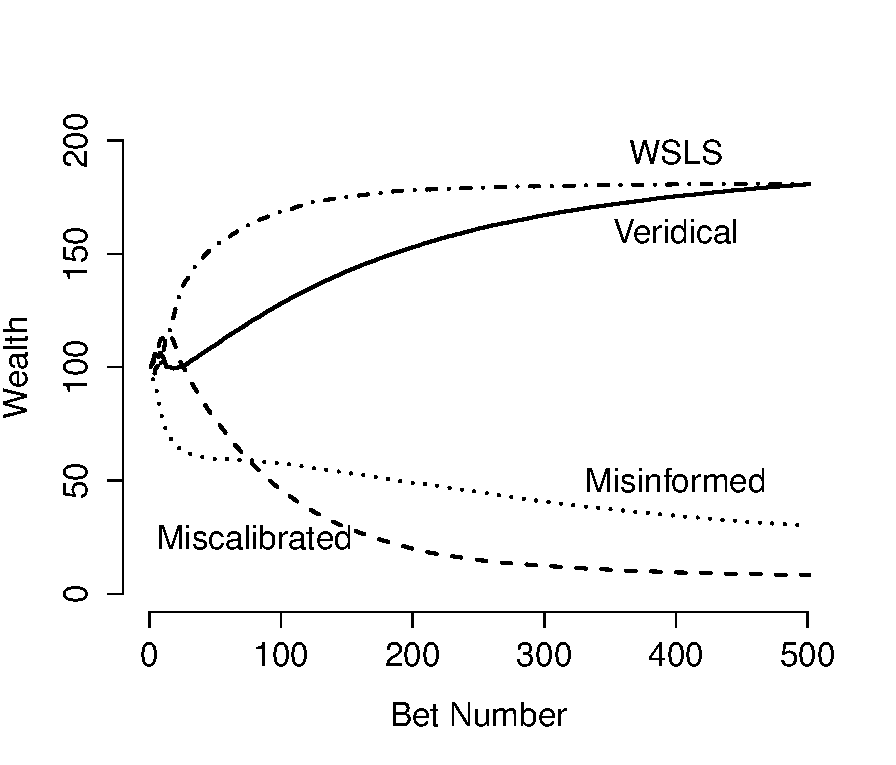
\includegraphics[width=.6\textwidth]{other_figs/threeBayesPlusWSLS.pdf}
	\caption{The gambling game from Figure~\protect\ref{fig:threeBayes} revisited, with a fourth non-Bayesian agent added to the mix. Despite its reliance on a simple win-stay lose-shift heuristic, the non-Bayesian agent is arguably the best gambler of the four. }
	\label{fig:gamblingRevisited}
\end{figure}

The conclusions from the simulations in Figure~\ref{fig:gamblingRevisited} mirror those from the original analysis---a Bayesian learner who solves the wrong problem has precious little guarantee of success in real life, and Dutch book arguments are a cold comfort to the exploited Bayesian---but extends it to highlight the fact that it is not at all easy to work out what the right problem should be. The correct solution to a {\it prediction} problem need not be the same as the solution to the corresponding {\it gambling} problem because the social environment is different. When making predictions one is not necessarily in competition with other agents, but gambling typically does put one in conflict with other people, and as a consequence the relative importance of social reasoning shifts quite dramatically. Labeling the veridical Bayesian model as ``optimal'' seems reasonable for a prediction task, but the same model is decidedly non-optimal at gambling. Of course, there is probably a Bayesian model that is ideal for the gambling problem---one that integrates social reasoning with objective learning in  a natural fashion---and we expect that this model would outperform all four of our existing models. However, this is beside the point. Our point here is that it is surprisingly easy to accidentally solve the wrong problem, and as a consequence we find ourselves very cautious about making optimality claims.

\subsection*{Combining Bayesian data analysis with Bayesian cognition}

Although not the main focus of our discussion, one theme that has run through some of our analysis is that it is useful to combine Bayesian models of human cognition with Bayesian data analysis tools---an approach that has been appropriately dubbed {\it doubly Bayesian} \cite{Huszar2010,Hemmer2014}. For example, in order to estimate individual subject response curves in case study 1 we implemented the  Bayesian cognitive model as a parameterized model in JAGS \cite{plummer_jags:_2003}, and the curves reported in Figure~\ref{fig:indiv} were constructed by plotting the model predictions at the posterior mean parameters. This is a fairly standard way of estimating model parameters within the Bayesian data analysis tradition \cite<e.g.,>{lee_bayesian_2014}. For the most part we have moved technical details to the Appendices, in order to make the main text more readable, but it is worth noting that much of what we are able to achieve in this paper has been because we relied on principled tools for model fitting and model selection, which the Bayesian data analysis approach provides.

The merits of combining a descriptive Bayesian cognitive model with a Bayesian data analysis are considerable. In principle, sophisticated data analysis methods are not necessary when building an optimal Bayesian model because there are no free parameters to be estimated---at least in theory if not so much in practice. The model is the very ideal of a scientific hypothesis because every relevant detail is specified a priori. This is a caricature of how optimal Bayesian models are constructed in the real world, but the issue of properly accounting for model complexity seems more important in situations where the researcher acknowledges that he or she does not know what priors or likelihoods the participant used.

In theory, Bayesian data analysis is naturally applicable to Bayesian cognitive models: The researcher expresses their uncertainty about the participant in the form of a {\it researcher prior}, and uses the Bayesian cognitive model to express the {\it researcher likelihood}. All inferences about individual participants and all model comparisons are then based on the {\it researcher posterior} beliefs about what actually happened in the experient. This is precisely the approach to data analysis advocated elsewhere in the methodological literature \cite<e.g.,>{lee_bayesian_2014,lee_three_2008,wagenmakers_practical_2007,kruschke_doing_2010}, but we concede that it poses a uniquely awkward problem when applied to Bayesian cognitive models: The same few words (``priors'', ``likelihoods'', ``posteriors'', etc) become severely overloaded. Authors must go to considerable rhetorical lengths to disambiguate between {\it participant priors} (what subjects believe about the world) and {\it researcher priors} (what the modeler believes about the subjects). Similarly, a {\it participant likelihood} would refer to the theory that underpins a participant's learning in the experiment, whereas the {\it researcher likelihood} refers to the researcher's theory about how participants were producing responses, and thus corresponds to the entirety of the Bayesian cognitive model. A good deal of care is required to clearly disambiguate between these different entities. Even so, our view is that the power of the Bayesian data analysis framework makes it worth the effort.


\subsection*{Conclusions}

Our goals in this paper are twofold. Most importantly, we argue that researchers need to make a clear distinction between Bayesian models that make normative claims and Bayesian models that make only descriptive claims. We feel that much of the confusion in the existing literature arises because people do not make this distinction as clearly as they should. As a secondary goal---because many researchers are unsure whether Bayesian models are useful when normative claims are not made---we have sought to highlight some of the types of questions and analyses that are possible while only making descriptive claims. Descriptive Bayesian models are more modest, because they require the researcher to express ignorance about which participant priors and participant likelihoods are involved. But it is exactly this modesty that makes them more generally useful, because the expression of researcher uncertainty is what allows the model to be used as a tool to guide our learning as psychologists. Instead of having to state {\it a priori} what knowledge people {\it should} have (priors) or what learning rules they {\it should} use (likelihoods), we treat those quantities as the unknowns that we seek to learn about.

Our three case studies, as simple as they are, illustrate several different ways in which descriptive Bayesian models can be used to learn about human cognition. The value of optimal models and normative descriptions have been debated elsewhere in the literature---it is arguably {\it the} central issue spanning the many papers that followed from the initial \citeA{jones_bayesian_2011} critique---but in our view the question of whether psychology needs {\it optimal} Bayesian models is very different to the question of whether {\it descriptive} Bayesian models are useful to the field.
Even the somewhat cursory applications we have presented in this paper illustrate the usefulness of these models for addressing a wide range of psychological questions that go beyond the narrow---albeit powerful---focus of optimal Bayesian models.

When combined with powerful statistical tools to perform inference (e.g., Bayesian data analysis, cross-validation, etc), we can use a flexible, descriptive Bayesian cognitive model to explore individual differences in prior beliefs and in the willingness to have data change those beliefs (case study 1). We can use them to learn about people's prior beliefs and how they compare to environmental statistics or to the performance of non-Bayesian heuristics (case study 2). Finally, we can develop tools that allow us to learn about the hypotheses that people rely on to guide their inferences (case study 3). Independent of the question about whether people's behavior is optimal, descriptive Bayesian models have an important role to play in helping us understand this behavior---which is, of course, one of the main goals of psychology.


\bibliographystyle{apacite}
\bibliography{references,zot3}



\section*{Appendix A: Details for the Bayesian gamblers problems}

In the main text we describe a gambling contest to determine which of three Bayesian agents holds ``better'' beliefs about a simple binary prediction task (e.g., whether the next card drawn from a deck will be black or white). The {\it veridical Bayesian} assumes---correctly, as it turns out---that arrivals are independent, and that there is some unknown probability $\theta = P(B)$ with which any given card will be black. Moreover, this Bayesian decides that they have no knowledge about $\theta$ and---again, correctly, as it turns out---places a uniform prior over this quantity $P(\theta) \propto 1$. The {\it misinformed Bayesian} also assumes that outcomes are independent, but adopts a prior that favours black  $P(\theta) \propto \theta$. Finally, the {\it miscalibrated Bayesian} correctly adopts a uniform prior over $\theta$ but incorrectly assumes that the arrivals will be ``streaky'', with successive arrivals tending to be of the same color. Specifically, the probability that the next card is black is judged to be $(\theta+1)/2$ if the last card was also black, but only $\theta/2$ if the last card was white. Formally, this likelihood arises from a first order Markov chain in which the marginal probability of black is fixed at $\theta$, but the probability that successive cards will be of different colors is only $\theta(1-\theta)$ rather than $2\theta(1-\theta)$ as would be expected if the outcomes were independent Bernoulli trials with probability $\theta$.

To convert this scenario into a gambling problem we suppose that every agent offers bets that they believe to be fair, and places a \$1 bet every time another agent offers a bet that they believe to be favorable. Given a starting stake of \$100, Figure~\ref{fig:threeBayes} tracks the relative fortunes of all three Bayesians, averaged across 10,000 repeats of the betting game. Critically, the game is structured to match the assumptions made by the first Bayesian: The true probability of a black card $\theta$ is generated uniformly at random on each repeat of the game, and the outcomes on every trial are generated independently on each trial. As the figure illustrates, the three Bayesians perform very differently on this problem: The misinformed Bayesian fares very poorly, and quickly loses money to the other two. The streaky Bayesian initially does well despite the miscalibrated likelihood but the veridical model tends to win out in the long run by capitalizing on the streaky model's tendency to expect too many repetitions and not enough alternations among the outcomes.

\section*{Appendix B: Details for the coincidences example}

In the original binary-data model for the coincidences task presented by GT1, the learner is told about a sample containing $n$ binary observations, of which $k$ are ``successes''. If the learner assumes the data represent the outcomes of $n$ independent Bernoulli trials, then the model described by Equations~\ref{eq:gt1-likelihood} and~\ref{eq:gt1-posterior} results. In our ``conservative'' version of the model the learner acts as if the effective sample size consisted of only $n^\prime$ observations, where $n^\prime \leq n$, and similarly assumes that there were only $k^\prime$ succeses where $k^\prime \leq k$. Thus the predictions of our model can be obtained by applying Equations~\ref{eq:gt1-likelihood} and~\ref{eq:gt1-posterior} to a smaller sample in which $k^\prime$ successes from $n^\prime$ trials are observed.

To formalize this in terms of a probabilistic model, we imagine that the learner ``retains'' only a subset of the original observations, where the probability that a specific observation is retained is denoted $\theta$. This model implies that the number of success observations retained $k^\prime$ and the number of non-success observations $n^\prime - k^\prime$ are both binomially distributed:
\begin{equation}
\begin{array}{rcl}
k^\prime & \sim & \mbox{Binomial}(\theta,k) \\
n^\prime - k^\prime &\sim& \mbox{Binomial}(\theta,n-k)
\end{array}
\end{equation}
Thus the full model has two free parameters to describe the response curve for an individual participant: $\theta$ captures the degree of conservatism (i.e., the extent to which data causes the learner to adjust his or her beliefs), and as per the original GT1 model, $\phi$ captures the prior degree of belief that the learner places in the alternative hypothesis (i.e., that a real effect exists). More precisely $\phi = \log P(h_1)/P(h_0)$ denotes the logarithm of the prior odds for the alternative hypothesis over the null.

The output of this model is the posterior probability $P(h_1 | n, k, \theta, \phi)$, the probability that the alternative hypothesis is true (according to the learner) given that observations $k$ out of $n$ successes were observed, given the learner's priors $\phi$ and likelihood $\theta$. If we let $e = P(h_1 | n, k, \theta, \phi)$ denote the extent of this evidence, then we assume that the actual response $r$ given by the participant is equal to this evidentiary value $e$ plus some normally distributed error:
\begin{equation}
r \sim \mbox{Normal}(e,\sigma_1^2)
\end{equation}
In our applications we defined the researcher prior over the response variability in terms of the precision (i.e., $\tau_1=1/\sigma_1^2$) and placed a diffuse prior over it, namely a $\mbox{Gamma}(.001,.001)$.

In order to specify a model that allows us to capture indvidual differences, we adopt a hierarchical Bayesian approach. We assume that each participant has unique value of $\theta$ and $\phi$, where these parameters are sampled from group level distributions:
\begin{equation}
\begin{array}{rcl}
\theta & \sim & \mbox{Beta}(a,b) \\
\phi & \sim & \mbox{Normal}(\mu,\sigma_2^2)
\end{array}
\end{equation}
The researcher prior over $a$ and $b$ is an exponential distribution with scale parameter 1. The prior over $\mu$ was a normal distribution with mean 0 and standard deviation 100, and the prior over the variability parameter $\sigma_2^2$ was again defined in terms of the precision, $\tau_2 = 1/\sigma_2^2$, where our prior over $\tau_2$ was again a $\mbox{Gamma}(.001,.001)$ distribution. We assume that different group level distributions exist for each of the cover stories. We implemented this as a graphical model in JAGS, allowing us to estimate the posterior distribution over $\theta$ and $\phi$ for each subject, as well as obtaining estimates of the group level parameters $a$, $b$, $\mu$, and $\sigma_2$. It is this model reported in the main text.

\section*{Appendix C: Details for the optimal predictions example}

The descriptive Bayesian model in the second case study uses the same likelihood function as the original model from GT2, but treats the participant prior as an unknown variable to be inferred from the data. To that end we assume that the learner's prior could be a normal distribution, an erlang distribution or a pareto distribution, and place a uniform (researcher) prior across these three possibilities:
\begin{equation}
t \sim \left\{
  \begin{array}{l l}
    \mbox{Normal}( \mu , \sigma ) & \quad \text{if $c=1$}\\
    \mbox{Erlang}( \beta ) & \quad \text{if $c=2$}\\
    \mbox{Pareto}( \gamma) & \quad \text{if $c=3$}
  \end{array} \right.
\end{equation}
where we (as researchers) place a uniform prior over $c$ and diffuse priors over the parameters for all three distributional families. Specifically our priors over the parameters are given by $\mu \sim \mbox{HalfNormal}(.0001)$ and $\sigma \sim \mbox{Uniform}(0,1000)$ for the normal distribution; $\beta \sim  \mbox{Uniform}(0,1000)$ for the erlang model; and $\gamma \sim \mbox{Gamma}(.1,.1)$ for the pareto distribution.

As noted in the main text, for any specific choice of paricipant prior the Bayesian cognitive model (both the descriptive model and the original optimal model from GT2) produces a paricipant posterior $P(t|x)$ corresponding to the learner's belief about the likely duration/extent of the unknown quantity. In order to convert this to a full probabilistic model for the participant response $r$ we assume that people sample the response from their posterior distribution. We implemented this model with a custom sampler in PyMC in order to estimate the posterior predictive estimates for the responses to each condition reported in Figure~\ref{fig:emp_vs_mink_agg_predictive}, as well as for the participant priors themselves (in Figure~\ref{fig:predictions-priors-subjective-vs-empirical}).

The Noisy \mink model is probabilistic extension of the \mink heuristic. The only difference in the new generative model is that instead of assuming that people report the value of $t$ that is produced by the \mink heuristic, it suggests that the participant samples their response from a normal distribution that is centered on that value. If $t^*$ denotes the value predicted by the deterministic \mink model, the Noisy \mink model predicts that people sample from
\begin{equation}
t \sim \mbox{Normal}(t^*,\sigma^2).
\end{equation}
However, since people never report values of $t$ that are below the observed value $x$, the actual response distribution is truncated at $x$. Moreover, instead of assuming that the experimenter guesses the value of the multiplier $g$, we fold it into the experimenter's model. That is, we specify a prior that captures our actual prior beliefs about the value of $g$,
\begin{equation}
g \sim \mathrm{Uniform}(0,3)
\end{equation}
and seek to infer the actual value of $g$ from the empirical data. As with the two Bayesian cognitive models, we implemented the model in PyMC and applied a custom sampler to infer posterior distributions over the model parameters $g$ and $\sigma$ as well as the specific exemplars people used to estimate $t^*$.

\section{Appendix D: Details for the generalization example}

As outlined in the main text, the Bayesian generalization model specified by TG1 specifies a {\it generalization probability}. When told that a set of items possesses some property, the generalization probability is the chance that a novel item shares that property. Given a binary matrix of category assignments $\mathbf{C}$---such that $c_{ix} = 1$ if item $i$ belongs to category $x$ and $c_{ix}=0$ if it does not---the simplest version of the model assumes that the extension of the novel property is to a single category. Under this model, the probability of generalizing a property from item $j$ to item $i$ is denoted $g(i|j)$,
\begin{equation}
\begin{array}{rcl}
g(i|j) &=& \sum_x P(c_{ix}=1) P(x | j)  \\
&=& \sum_{x | c_{ix}=1} P(x | j)
\end{array}
\end{equation}
where $P(x|j)$ is the posterior probability that category $x$ is the true extension of the novel property given that the item $j$ is known to possess the property, and
\begin{equation}
P(x|j) \propto P(j|x) P(x)
\end{equation}
The prior distribution $P(x)$ is captured by a vector of weights $\mathbf{w}$ such that $w_x \geq 0$ and $\sum_x w_x = 1$. As discussed in the main text, the likelihood function is a weighted mixture of the strong sampling model and the weak sampling model, so the probability that item $j$ would have been generated if $x$ were the true hypothesis is given
\begin{equation}
P(j|x) = (1-\theta) \frac{1}{n} + \theta \frac{c_{jx}}{n_x}
\end{equation}
where $n_x = \sum_j c_{jx}$ counts the number of item is the $x$-th category, $n$ is the total number of items in the domain, and $\theta$ is a model parameter that specifies which sampling model the learner relies upon: $\theta=0$ implies weak sampling and $\theta=1$ is strong sampling.

The full model implemented in the paper extends this basic model in four respects. Firstly, following TG1 we allow generalization from multiple exemplars, so if the learner has been told that items $j$ and $k$ both possess the novel property, the posterior probability of category $x$ is given by
\begin{equation}
P(x|j,k) \propto P(j|x) P(k|x) P(x)
\end{equation}

Secondly, the ``base'' category matrix $\mathbf{C}$ is augmented by one ``universal'' category (to which all items belong) and $n$ ``singleton'' categories (each containing only one item). So if $\mathbf{C}$ is an $n \times m$ binary matrix specifying the memberships for $m$ categories, then the model actually has $m+n+1$ categories once the universal and singleton categories are added. As such the weights vector $\mathbf{w}$ that specifies the prior distribution over categories has length $m+n+1$.

The third extension allows the learner to construct a more elaborate hypothesis space $\mathcal{H}$ from the base representation defined by $\mathbf{C}$ and $\mathbf{w}$. Instead of assuming that the extension of the unknown property is necessarily restricted to a single category, the learner also consider the possibility that the property is possessed by the members of two categories (i.e., the intersection of two categories in $\mathbf{C}$. We operationalize this in terms of an expanded hypothesis matrix $\mathbf{H}$ that contains a copy of every element in $\mathbf{C}$ as well as an additional column for every pair of columns in $\mathbf{C}$, and whose elements are 1 if {\it either} of the original columns has a 1 in the corresponding location. The prior probability of any such ``composite'' hypothesis is computed from the weights vector $\mathbf{w}$ in the following way. If hypothesis $z$ is the union of categories $x$ and $y$ then
\begin{equation}
P(z) \propto \gamma w_x w_y
\end{equation}
and similarly if hypothesis $z$ is a ``primitive'' hypothesis that corresponds to category $x$ only then
\begin{equation}
P(z) \propto (1-\gamma) w_x
\end{equation}

Finally, in order to assign probability to responses at an individual trial level we assume that the raw response is sample from a normal distribution whose mean corresponds to the model-predicted generalization probability, $g(i|j)$ or $g(i|j,k)$, and whose variance $\sigma^2$ is unknown.

The full model is requires that we infer an $n \times m$ binary matrix $\mathbf{C}$ for the category assignments, a vector of $n+m+1$ non-negative weights $\mathbf{w}$ for the $m$ base categories, the $n$ singleton categories and the 1 universal categories (though this corresponds only to $n+m$ unknowns as these must sum to 1), the parameter $\theta$ that defines the sampling model and the parameter $\gamma$ that indicates the relative weights assigned to ``primitive'' versus ``composite'' hypotheses. To perform inference in this model we specify researcher priors for $\theta$ and $\gamma$ that are uniform across the unit interval, uniform priors across all possible binary matrices $\mathbf{C}$ (for a fixed value of $m$) and uniform across weight vectors $\mathbf{w}$. We used a simulated annealing algorithm to find the best fitting (i.e., maximum a posteriori) values for the theoretically relevant parameters $\mathbf{C}$, $\mathbf{w}$, $\theta$ and $\gamma$. Following \citeA{tenenbaum_learning_1996} we treated $\sigma^2$ as a nuisance parameter, and can be used as a de facto temperature parameter in a simulated annealing algorithm by initalizing $\sigma^2$ at a large value and gradually reducing it. The results reported in the main text were the result of an application of the simulated annealing procedure with $m=8$.

It should be noted that unlike the other two cases studies we did not do full Bayesian inference for this model. What we have reported is a point estimate (in effect the Bayesian MAP estimate) for the theoretically important variables, rather than estimating the full posterior distribution over all variables. The reason for this is partly that it is more tractable to compute the point estimate, though not impossible: We did also implement a fully Bayesian version of a restricted model that more closely resembles the approach in \citeA{navarro2008}, and found it worked reasonably well. The more important reason is that the results are somewhat more interpretable when we have a {\it single} set of categories $\mathbf{C}$, rather than a full posterior distribution over possible category assignment matrices. The former can be described in a table, the latter is difficult to summarize, though \citeA{navarro2008} do offer suggestions for how to do so.

\end{document}

